%!TeX spellcheck = de_DE

\providecommand{\additionalOptionsForClass}{}
\documentclass[
  accentcolor=tud1c,	% Color theme for TUD corporate design
  colorbacktitle,		% Titlepage has colored background for title area
  inverttitle,			% Font color of title on titlepage is inverted
  \additionalOptionsForClass
  %german%,
  %twoside
]{tudexercise}

\parindent1em
%\parskip2ex

\usepackage[ngerman]{babel}
\usepackage[utf8]{inputenc}
\usepackage{listings}
\usepackage{booktabs}
\usepackage{amsmath}
\usepackage{algorithm2e}
\usepackage{hyperref}
\usepackage{xspace}
\usepackage{tabularx}
\usepackage{tikz}
\usepackage{cleveref}
\usepackage{numprint}
\usepackage{paralist}
\usepackage{verbatim}
\usepackage{tocloft} % for manipulating the table of contents

\usetikzlibrary{shapes}
\usetikzlibrary{calc}
\usetikzlibrary{arrows}
\usetikzlibrary{decorations}

\usepackage{pifont}
\newcommand{\cmark}{\ding{51}\xspace}%
\newcommand{\xmark}{\ding{55}\xspace}%

\usepackage{todonotes}
%\usepackage[disable]{todonotes} % Use this line to hide all todos

\definecolor{commentgreen}{RGB}{50,127,50}
\lstloadlanguages{C++,[gnu]make}
\lstset{language=C++}
\lstset{captionpos=b}
\lstset{tabsize=3}
\lstset{breaklines=true}
\lstset{basicstyle=\ttfamily}
\lstset{columns=flexible}
\lstset{keywordstyle=\color{purple}}
\lstset{stringstyle=\color{blue}}
\lstset{commentstyle=\color{commentgreen}}
\lstset{otherkeywords=\#include}
\lstset{showstringspaces=false}
\lstset{keepspaces=true}
\lstset{xleftmargin=1cm}
\lstset{literate=%
	{Ö}{{\"O}}1
	{Ä}{{\"A}}1
	{Ü}{{\"U}}1
	{ß}{{\ss}}2
	{ü}{{\"u}}1
	{ä}{{\"a}}1
	{ö}{{\"o}}1
	{'}{{\textquotesingle}}1
}

\lstnewenvironment{lstmake} %
{\lstset{language=[gnu]make}} %
{}


\newcommand{\superscript}[1]{\ensuremath{^{\textrm{#1}}}}
\newcommand{\subscript}[1]{\ensuremath{_{\textrm{#1}}}}

\newcommand{\setHeader}[1]{
\providecommand{\examheadertitle}{TODO: Titel einbinden}
\renewcommand{\examheadertitle}{#1}
\begin{examheader}
    \examheadertitle
\end{examheader}
}

\newcommand{\hints}[1]{
\paragraph*{Hinweise}
	\begin{itemize}
		\setlength{\itemsep}{0pt}
		#1
	\end{itemize}
}

\newcommand{\optional}{\xspace(optional)}
\newcommand{\experimental}{\xspace(experimentell)}

\usepackage{fancybox}
\newcommand{\optionaltextbox}{
	\bigskip
	\begin{center}
		\ovalbox{\parbox{0.98\textwidth}{Die Klausur kann ohne diese Aufgabe bestanden werden. Wir empfehlen aber sie trotzdem zu bearbeiten.}}
	\end{center}
}
\newcommand{\experimentaltextbox}{
	\bigskip
	\begin{center}
		\ovalbox{\parbox{0.98\textwidth}{Diese Aufgabe wurde neu erstellt und kann noch Fehler und Inkonsistenzen enthalten. Falls euch etwas derartiges auffällt sprecht uns bitte darauf an oder stellt es auf GitHub in den Issuetracker unter \url{https://github.com/Echtzeitsysteme/tud-cpp-exercises/issues}}}
	\end{center}
}

\newcommand{\enquote}[1]{\glqq#1\grqq\xspace}
\newcommand{\filename}[1]{\texttt{#1}}

\newcommand{\RK}[1]{\todo[]{\textbf{RK:} #1}}
\newcommand{\RKi}[1]{\todo[inline]{\textbf{RK:} #1}}

\newcommand{\ExercisePrefix}[1]{$[$#1$]$ \xspace}
\newcommand{\ExercisePrefixBasics}{\ExercisePrefix{G}}
\newcommand{\ExercisePrefixMemory}{\ExercisePrefix{S}}
\newcommand{\ExercisePrefixObjectOrientation}{\ExercisePrefix{O}}
\newcommand{\ExercisePrefixAdvanced}{\ExercisePrefix{F}}
\newcommand{\ExercisePrefixEmbeddedC}{\ExercisePrefix{C}}
\newcommand{\ExercisePrefixElevator}{\ExercisePrefix{A}}
\newcommand{\ExercisePrefixAdditionalInformation}{\ExercisePrefix{Z}}

\title{Übung zum\linebreak[1]C/C++-Praktikum\linebreak[1] Fachgebiet Echtzeitsysteme}

\setcounter{section}{0}

%optional parameters to speed up build (increases pdf file size)
%\pdfcompresslevel=0
%\pdfobjcompresslevel=0
\begin{document}

% header and title
\maketitle

\noindent\emph{Hinweis:} Die Präfixe der Aufgaben beziehen sich auf die Themengebiete der Vorlesung. (%
\ExercisePrefixBasics{}: Grundlagen; 
\ExercisePrefixMemory{}: Speicherverwaltung/Memory;
\ExercisePrefixObjectOrientation{}: Objektorientierung;
\ExercisePrefixAdvanced{}: Fortgeschrittene Themen;
\ExercisePrefixEmbeddedC{}: (Embedded) C;
\ExercisePrefixElevator{}: Zusatzaufgaben zum Aufzugsimulator
)
\setcounter{tocdepth}{1}
%\setlength\cftsectionnumwidth{10em}
\setlength\cftsecnumwidth{10em}
\setlength\cftbeforesecskip{.1em} % line skip between sections ("sec")
\tableofcontents

\vspace*{\fill}
\cclicense

\newpage

%\begin{comment}
\setHeader{Aufgaben zu C/C++-Grundlagen}
\section*{Einführung}
Für alle Übungen des C/C++ Praktikums wird CodeLite als IDE verwendet. Als Compiler kommt Clang zum Einsatz.
Eine Einführung in den Umgang mit CodeLite findet am ersten Praktikumstag statt.

Die Materialien zur Vorlesung und Übung sind in zwei Git-Repositories zu finden.
Diese beinhalten zum einen die Folien und die Programmbeispiele aus der Vorlesung und zum anderen diese Übungsblätter, Vorlagen für die letzten beiden Tage des Praktikums und alle Lösungen zu den Übungsaufgaben.

\begin{itemize}
	\item \textbf{Vorlesung:} \url{https://github.com/Echtzeitsysteme/tud-cpp-lecture}
	\item \textbf{Übungen/Git- und CodeLite-Einführung:} \url{https://github.com/Echtzeitsysteme/tud-cpp-exercises}
\end{itemize}

Falls du mit dem Übungsblatt für den dafür vorgesehenen Tag innerhalb der Präsenzzeit fertig werden solltest kannst du außerdem gerne mit dem nächsten Übungsblatt anfangen.

\hints{
	\item Bei Fragen und Problemen aktiv um Hilfe bitten!
	\item Alle Lösungen enthalten ein Makefile und können entweder über die
Kommandozeile mit Hilfe von \lstinline{make} kompiliert werden, oder in CodeLite, indem du sie als Projekt importierst.
	\item Folgende Shortcuts könnten sich dir im Verlauf des Praktikums als nützlich erweisen:
}


\begin{tabular}{l|l|p{11.5cm}}
    \toprule
    \textbf{Tastenkürzel} & \textbf{Befehl} & \textbf{Beschreibung}\\
    \midrule
	Ctrl+Space & Autocomplete &
	Anzeige von Vervollständigungshinweisen (z.B. nach \texttt{std::} oder \texttt{main})
	\\
	Alt+Shift+L & Rename local &
	Umbennenen von lokalen Variablen
	\\
	Alt+Shift+H & Rename symbol &
	Umbennenen von Funktionen und Klassen
	\\
	Ctrl+N & New &
	Anlegen neuer Datei
	\\
	F12 & Switch tab &
	Wechsel zwischen der Header- und der Implementierungsdatei
	\\
	F7 & Build &
	Startet den Buildprozess (Aufruf von Compiler und Linker)
    \\\bottomrule
\end{tabular}


\section*{Musterlösungs-/Microcontroller-Projekte in CodeLite importieren}

Die angebotenen Musterlösungs-/Microcontroller-Projekte basieren auf Makefiles.
Daher ist es wichtig, dass du sie entsprechend importierst: \textbf{Workspace -> Add an existing project} und dann zur entsprechenden \filename{.project}-Datei navigieren.


\section{Hello World}
Lege ein neues C++ Projekt an, indem du \textbf{Workspace $\rightarrow$ New project} im CodeLite Menü wählst und als Projekttyp \textbf{CPPP/C++ Projekt} auswählst.
Wähle einen passenden Projektnamen, z.b. \texttt{Tag1\_Aufgabe1}. Als Projektpfad sollte \texttt{/home/cppp/CPPP/Workspace} ausgewählt sein. Achte darauf, dass der Haken bei \texttt{Create the project under a separate directory} gesetzt ist.

Das Projekt enthält bereits eine Datei \texttt{src/main.cpp}. Erweitere die \texttt{main}-Funktion wie gezeigt und kompiliere das Projekt mit einem Klick auf das Build-Symbol (grünes Rechteck mit weißem Pfeil). Führe dann das Programm mit einem Klick auf das Zahnrad-Symbol aus.

% fix that avoids undesired page breaks
\begin{minipage}{\textwidth} 
	\lstinputlisting{01_basics/problems/listings/helloworld.cpp}
\end{minipage}

Jedes vollständige C++ Programm muss \textbf{genau eine} Funktion mit Namen \lstinline{main} und Rückgabetypen \lstinline{int} außerhalb von Klassen im globalen Namensraum besitzen.
Andernfalls wird der Linker mit der Fehlermeldung \emph{undefined reference to 'main'} abbrechen.
Der Rückgabetyp wird verwendet um dem Aufrufer (Betriebssystem, Shell, \dots) den Erfolg oder Misserfolg der Ausführung zu signalisieren.
Typischerweise wird im Erfolgsfall 0 zurückgegeben.

Die erste Zeile des obigen Programms bindet den Header der \lstinline{iostream} Bibliothek ein, welche unter anderem Klassen und Funktionen zur Ein- und Ausgabe mit Hilfe von $<<$ (\emph{insertion operator}) und $>>$ (\emph{extraction operator}) anbietet.
Diese Bibliothek ist Teil der C++-Standardbibliothek, welche eine Sammlung an generischen Containern, Algorithmen und vielen häufig genutzten Funktionen ist.
Um auf die Elemente dieser Bibliothek zuzugreifen, muss man ihren \lstinline{namespace} (in diesem Fall \lstinline{std}) voranstellen, gefolgt von zwei Doppelpunkten und dem gewünschten Element (in diesem Fall \lstinline{cout} und \lstinline{endl}).
Um Überschneidungen mit eigenen Definitionen zu vermeiden, ist es üblich Bibliotheken in einem \lstinline{namespace} zu kapseln, welcher analog zu \lstinline{package} in Java funktioniert, jedoch nicht an Ordnerstrukturen gebunden ist.

In der dritten Zeile wird der String \lstinline{"Hello World"} in \lstinline{std::cout} eingefügt, gefolgt von \lstinline{std::endl}, das einen Zeilenumbruch erzeugt und die Ausgabepuffer leert. Für weitere Informationen zur Kommandozeilenausgabe siehe \url{http://www.cplusplus.com/doc/tutorial/basic_io/} und \url{http://www.cplusplus.com/reference/iomanip/}.

\hints{
	\item Einzeilige Kommentare können durch \lstinline{//}, mehrzeilige durch \lstinline{/* ... */} eingeschlossen werden.
	\item Anders als in Java können Funktionen auch außerhalb von Klassen definiert und verwendet werden.
	\item Die \lstinline{return} Anweisung darf in der \lstinline{main} Funktion weggelassen werden.
}

\subsection*{Häufige (Compiler-)Fehlermeldungen}

Im Folgenden sind einige Fehlermeldungen von \texttt{clang} zusammen mit möglichen Lösungsstrategien aufgelistet.
Die generelle Faustregel lautet: 
\textbf{Kompilierfehler sollten immer von oben nach unten abgearbeitet werden, so wie sie in der Konsole erscheinen.}
Der Grund hierfür ist, dass es durch einen Fehler zu weiteren Folgefehlern kommen kann.

% Indents all of the following paragraphs by 1cm

\begin{verbatim}
  main.exe: not found
\end{verbatim}

Dieser Fehler wird von CodeLite geworfen, wenn es nach dem Kompilieren das lauffähige Programm nicht findet.
Das kann zwei Gründe haben:
\begin{itemize}
\item Der Kompiliervorgang ist gescheitert. Prüfe die \texttt{Console} auf Fehler.
\item Der Kompiliervorgang wurde noch nicht ausgeführt. Kompiliere das Programm mit einem Klick auf das Build-Symbol.
\end{itemize}

\begin{verbatim}
  error: expected ';' before ...
\end{verbatim}

Dies bedeutet, dass in der Zeile davor ein \textbf{;} vergessen wurde.
Allgemein beziehen sich Fehlermeldungen \textbf{expected ... before ...} häufig auf die Zeile \textbf{vor} dem markierten Statement.
Beachte, dass \emph{die Zeile davor} auch die letzte Zeile einer eingebundenen Header-Datei sein kann. Beispiel:

\lstinputlisting{01_basics/problems/listings/helloworld_error_main.cpp}

Falls im Header \filename{main.h} in der letzten Zeile ein Semikolon fehlt, wird der Compiler die Fehlermeldung trotzdem auf die Zeile \glqq{}\lstinline{int main() {}\grqq{} beziehen!!

\begin{verbatim}
  error: invalid conversion from <A> to <B>.
\end{verbatim}

Dies bedeutet, dass der Compiler an der entsprechenden Stelle einen Ausdruck vom Typ \emph{B} erwartet, im Code jedoch ein Ausdruck vom Typ \emph{A} angegeben wurde. Insbesondere bei verschachtelten Typen sowie (später vorgestellten) Zeigern und Templates kann die Fehlermeldung sehr lang werden. In so einem Fall lohnt es sich, den Ausdruck in mehrere Teilausdrücke aufzubrechen und die Teilergebnisse durch temporäre Variablen weiterzureichen.

\begin{verbatim}
  undefined reference to ...
\end{verbatim}

Dies bedeutet, dass das Programm zwar korrekt kompiliert wurde, der Linker aber die Definition des entsprechenden Bezeichners nicht finden kann.
Das kann passieren, wenn man dem Compiler durch einen Prototypen mitteilt, dass eine bestimmte Funktion existiert (\textbf{deklariert}), diese aber nirgendwo tatsächlich \textbf{definiert}.
Überprüfe in diesem Fall, ob der Bezeichner tatsächlich definiert wurde und ob die Signatur der Definition mit dem Prototypen übereinstimmt.

\newpage
\section{C++ Grundlagen, Funktionen und Strukturierung}
Für diese Aufgabe kannst du entweder das vorherige Programm weiter entwickeln oder genauso wie vorher ein neues Projekt anlegen.

\subsection*{Primitive Datentypen} 
Die primitiven Datentypen in C++ sind ähnlich denen in Java.
Allerdings sind alle Ganzzahl-Typen in C++ sowohl mit als auch ohne Vorzeichen verfügbar.
Standardmäßig sind Zahlen vorzeichenbehaftet.
Mittels \lstinline{unsigned} kann man vorzeichenlose Variablen deklarieren.
Durch das freie Vorzeichenbit kann ein größerer positiver Wertebereich dargestellt werden.

\begin{lstlisting}
int i;						// signed int, -2147483648 to +2147483647 on a 32-bit machine
unsigned int ui;			// unsigned int, 0 to 4294967295 on a 32-bit machine
// unsigned double d;	// not possible
\end{lstlisting}

Eine andere Besonderheit von C++ ist, dass Ganzzahlwerte implizit in Boolesche Werte (Typ: \lstinline{bool}) umgewandelt werden.
Alles ungleich 0 wird als \lstinline{true} gewertet, 0 als \lstinline{false}.
Somit können Ganzzahlen direkt in Bedingungen ausgewertet werden.

\subsection{Größe von Datentypen}
Die Größe von den verschiedenen Datentypen ist essentiell zu wissen, wenn man mit ihnen arbeiten möchte.
Deshalb sollst du dir in dieser Aufgabe die Größe der folgenden Datentypen in Bits, wie auch deren minimalen und maximalen Wert ausgeben lassen.

\begin{lstlisting}
    int
    unsigned int
    double
    unsigned short
    bool
\end{lstlisting}

\hints{
    \item Zum Überprüfen der Größe von Datentypen kann man den \lstinline{sizeof()} Operator\footnote{\url{http://en.cppreference.com/w/c/language/sizeof}} verwenden.
    \item Die C++ Klasse \lstinline{std::numeric\_limits}\footnote{\url{http://en.cppreference.com/w/cpp/types/numeric_limits}} bietet Funktionen sich minimale und maximale Werte von Datentypen ausgeben zu lassen. 
Einbinden lässt sich diese über den Header \lstinline{limits}.
}

\subsection{Sternmuster mit Funktionen malen}

Schreibe eine Funktion \lstinline{printStars(int n)}, die \lstinline{n}-mal ein * auf der Konsole ausgibt und mit einem Zeilenumbruch abschließt.
Ein Aufruf von \lstinline{printStars(5)} sollte folgende Ausgabe generieren:

\begin{lstlisting}
*****
\end{lstlisting}

Platziere die Funktion \textbf{vor} der \lstinline{main}, da sie sonst von dort aus nicht aufgerufen werden kann.
Benutze die erstellte Funktion \lstinline{printStars(int n)}, um eine weitere Funktion zu schreiben, die eine Figur wie unten dargestellt ausgibt.
Verwende hierzu Schleifen.

\begin{lstlisting}
*****
****
***
**
*
**
***
****
*****
\end{lstlisting}

\hints{
    \item Was die Benennung von Funktionen, Variablen und Klassen angeht, bist du frei. Für Klassen ist \enquote{CamelCase} wie in Java üblich. Bei Funktionen und Variablen wird zumeist entweder auch Camel Case oder Kleinschreibung mit Unterstrichen verwendet.
    \item Um Strings auszugeben, stellt dir C++ \lstinline{std::cout} zur Verfügung, welches den String zu dem Standart Output Stream weitergibt. Diesen Output Stream kann man mit dem Manipulator \lstinline{std::endl} zu einem Zeilenumbruch zwingen.
}

\subsection{Auslagern der Datei}
Erstelle eine neue Header-Datei \filename{functions.hpp} und eine neue
Sourcedatei \filename{functions.cpp}.
Klicke hierzu mit der rechten Maustate auf den Ordner \textbf{src} und wähle \textbf{New class}, gib einen Klassennamen ein und bestätige den Dialog mit \textbf{OK}. Alle anderen Felder werden automatisch ausgefüllt oder können leer bleiben.
Beachte hierbei, dass CodeLite automatisch Include-Guards in der Headerdatei erzeugt, die das mehrfache Einbinden desselben Headers verhindern:

\begin{lstlisting}
#ifndef FUNCTIONS_HPP_
#define FUNCTIONS_HPP_
// your header ...
#endif /* FUNCTIONS_HPP_ */
\end{lstlisting}

Binde danach \filename{functions.hpp} in beide Sourcedateien ein indem du

\begin{lstlisting}
#include "functions.hpp"
\end{lstlisting}

verwendest.
\textbf{Verschiebe} deine beiden Funktionen nach \filename{functions.cpp}.

Schreibe nun in \filename{functions.hpp} \textbf{Funktionsprototypen} für die beiden Funktionen aus der vorherigen Aufgabe.
Funktionsprototypen dienen dazu, dem Compiler mitzuteilen, dass eine Funktion mit bestimmtem Namen, Parametern und Rückgabewert existiert.
Ein Prototyp ist im wesentlichen eine mit \textbf{;} abgeschlossene Signatur der Funktion ohne Funktionsrumpf.
Der Prototyp von \lstinline{printStars(int n)} lautet 
\begin{lstlisting}
void printStars(int n);
\end{lstlisting}

Fertig -- die Ausgabe des Programms sollte sich nicht verändert haben.

\hints{
	\item Sourcedateien tragen in der Regel die Endung \filename{.cpp}, Headerdateien \filename{.h} oder \filename{.hpp}.
	\item Denke daran, auch in \filename{functions.cpp} den Header \lstinline{iostream} einzubinden, falls du dort Ein- und Ausgaben verwenden willst (\lstinline{#include<iostream>}).
	\item Beachte, dass es zwei verschiedene Möglichkeiten gibt, eine Header-Datei einzubinden - per \lstinline{\#include <Bibliotheksname>} sowie per \lstinline{\#include "Dateiname"}.
    Bei der ersten Variante sucht der Compiler nur in den Include-Verzeichnissen der Compiler-Toolchain, während bei der zweiten Variante auch die Projektordner durchsucht werden. Somit eignet sich die erste Schreibweise für System-Header und die zweite für eigene, projektspezifische Header.
	\item Anstelle der Include-Guards kannst du auch die Präprozessordirektive \lstinline{\#pragma once} verwenden. Dies wird von den meisten Compilern unterstützt.
}

\subsection{Dokumentation} \label{basics:doc}
Für die Lesbarkeit eines Programms ist eine ausführliche Dokumentation des Programmcodes essentiell.
Damit ihr schonmal einen Einblick darin bekommt, werden wir hier in dem Praktikum mit kommentieren und das Tool \emph{Doxygen}\footnote{Doxygen-Link als Referenz: \url{http://www.doxygen.nl/}} zur Erstellung von Dokumentationen verwenden.

Damit Doxygen deine Kommentare erkennt, müssen sie ein spezielles Format einhalten.
\begin{itemize}
    \item Die Kommentare vor den jeweiligen zu kommentierenden Elementen (z.B. Funktionen) stehen.
    \item{Mehrzeilige Kommentare müssen den folgenden Stil einhalten (beachte hierbei das zusätzliche \lstinline{*} in der ersten Zeile)
        \begin{lstlisting}
/**
 * Content
 */
        \end{lstlisting}}
\end{itemize}

Außerdem müssen bestimmte Kommandos in den Kommentaren verwendet werden, die Doxygen bei der Dokumentationsgenerierung verwenden kann.
Diese Kommandos sind die folgenden

\begin{itemize}
    \item \lstinline{@brief kurzeBeschreibung} einzeilige Beschreibung des Elements.
    \item \lstinline{@author AuthorenNamen} für den Namen des Autoren.
    \item \lstinline{@name Funktionsnamen} für den Namen der Funktion.
    \item \lstinline{@param Parametername Beschreibung} um Parameterübergaben bei Funktionen zu erklären.
    \item \lstinline{@return Beschreibung} kurze Beschreibung der Rückgabe.
    \item \lstinline{@file Dateiname} damit Doxygen den kompletten File parst.
\end{itemize}

Da das Dokumentieren der Datei nicht vor der Datei passieren kann (wo sollte das sein?), geschieht es deshalb direkt nach den Präprozessor Direktiven.

Eure Aufgabe ist es nun, den von euch erstellten Code sorgfältig zu dokumentieren.
Die Dokumentation geschieht dabei in der \filename{.h} oder \filename{.hpp} Datei.

Hier ein kleines Beispiel dazu, damit ihr eine Vorstellung davon bekommt, wie das ganze am Ende auszusehen hat.

\begin{lstlisting}
#ifndef TESTING_HPP_
#define TESTING_HPP_

/**
 * @file testing.hpp
 * @author Your Name
 * @brief Just a showcase hpp file to demonstrate doxygen comments
 */

/**
 * @name first_func(int a);
 * @author Your Name
 * @brief A showcase function.
 * @param a Used for important stuff.
 * @return void
 */
void first_func(int a);

/**
 * @name second_(int a, char b, double d);
 * @author Your Name
 * @brief A showcase function.
 * @param a Used for important stuff.
 * @param b Used for important stuff.
 * @param d Used for important stuff.
 * @return void
 */
void second_func(int a, char b, double d);

#endif /* TESTING_HPP_ */
\end{lstlisting}

Erstellen könnt ihr die Dokumentation am Ende über die Kommandozeile.
Dafür öffnet ihr euer Terminal mit \lstinline{STRG + ALT + t} und wechselt in das Verzeichnes in dem euer Projekt liegt (üblicherweise \lstinline{cd CPPP/Workspace/NameEuresProjektes}).
Dort gebt ihr \lstinline{doxygen -g} ein, welches euch eine vorgefertigte Konfigurationsdatei von \texttt{doxygen} erstellt, gefolgt von \lstinline{doxygen}, was letztendlich die Dokumentation erstellt.
Diese findet ihr in dem Ordner \filename{html} unter der Datei \filename{index.html}.
Ihr erreicht die Datei ganz einfach, wenn ihr in der Terminal das Kommando \lstinline{pcmanfm} eingebt, was euren Filemanager öffnet.
Auf der Webseite, die sich dann öffnet, findet ihr unter Files die von euch dokumentierte \filename{functions.{h,hpp}}.

\subsection{Eingabe}
Erweitere das Programm um eine Eingabeaufforderung zur Bestimmung der Breite der auszugebenden Figur.
Die Breite soll dabei eine im Programmcode vorgegebene Grenze nicht überschreiten dürfen.
Gib gegebenenfalls eine Fehlermeldung aus.
Verwende zum Einlesen \lstinline{std::cin} und \lstinline{operator>>} wie in folgendem Beispiel.

\begin{lstlisting}
int x;
std::cin >> x; // Type, e.g., 174 and press ENTER.
// Now, x contains the entered number.
std::cout << x << std::endl.
\end{lstlisting}

Erstelle auch für diesen Aufgabenteil eine eigene Funktion und lagere diese nach \filename{functions.cpp} aus.

\subsection{Fortlaufendes Alphabet ausgeben}
Statt eines einzelnen Zeichens soll nun das fortlaufende Alphabet ausgegeben werden.
Sobald das Ende des Alphabets erreicht wurde, beginnt die Ausgabe erneut bei \emph{a}.
Beispiel:

\begin{lstlisting}
abc
de
f
gh
ijk
\end{lstlisting}

Implementiere dazu eine Funktion \lstinline{char nextChar()}.
Diese soll bei jedem Aufruf das nächste auszugebende Zeichen von Typ \lstinline{char} zurückgeben, beginnend bei \emph{a}.
Dazu muss sich \lstinline{nextChar()} intern das aktuelle Zeichen merken.
Dies kann durch die Verwendung von statischen Variablen erreicht werden. Diese behalten ihren alten Wert beim Wiedereintritt in die Funktion.
Ein statische Variable \lstinline{c} wird mittels

\begin{lstlisting}
static char c = 'a';
\end{lstlisting}

deklariert.
In diesem Fall wird die Variable \lstinline{c} \textbf{einmalig zu Beginn des Programms} mit \lstinline{'a'} initialisiert und kann später beliebig verändert werden.

\hints{
	\item Der Datentyp \lstinline{char} kann wie eine Zahl verwendet werden, d.h. man kann z.B. die Modulooperation \lstinline{\%} verwenden.
}

\subsection{Namensräume}
Bibliotheken werden in einen eigenen Namensraum gekapselt, damit ihre Funktionen nicht mit gleichnamigen Funktionen in anderen Bibliotheken kollidieren.
Erweitere dazu das Programm, indem du im Header die Funktionsprototypen wie
folgt in einen \lstinline{namespace} setzt.

\begin{lstlisting}
namespace fun {
	// function prototypes ...
};	// semicolon!
\end{lstlisting}

Denke daran, dass du die Namen der Funktionen in der Sourcedatei noch anpassen musst, indem du vor jede Funktion den gewählten \lstinline{namespace}-Namen gefolgt von zwei Doppelpunkten setzt.
Genauso muss der Namensraum vor jedem Aufruf der Funktion gesetzt werden.

\begin{lstlisting}
void fun::print_star(int n) {
	// ...
}
\end{lstlisting}

Vergisst man, den Namensraum in der Sourcedatei anzugeben, findet der Linker keine Implementation zu der im Header definierten Funktion.
Weiterhin stünde diese Funktion nicht mehr im Bezug zum Header und könnte nur noch lokal verwendet werden (\lstinline{print_star(int n)} und \lstinline{fun::print_star(int n)} sind unterschiedliche Funktionen!). \\ \smallskip

Falls man seine Funktionen noch weiter unterteilen möchte, kann man Namensräume auch schachteln.
Hierzu definiert man wie oben ein weiteren Namensraum mit \lstinline{namespace} in einer anderen Namensraum Instanz.

\begin{lstlisting}
namespace fun {
    namespace ny{
	// function prototypes ...
    };	// semicolon!
};	// semicolon!
\end{lstlisting}

In der Sourcedatei folgt dann nach dem initialen Namensraum, hier \lstinline{fun} gefolgt von dem Doppelpunktpaar, der geschachtelte Namensraum \lstinline{ny} wieder gefolgt von zwei Doppelpunkten.
Erst dann können die Funktionen in dem Namensraum \lstinline{ny} verwendet werden.

\begin{lstlisting}
void fun::ny::print_star(int n) {
	// ...
}
\end{lstlisting}

In diesem Projekt wird dies nicht notwendig sein, da die Anzahl der definierten Funktionen überschaubar ist, aber trotzdem empfehlen wir dir es auszuprobieren.

\hints{
	\item Du kannst \lstinline{using namespace fun;} verwenden, um diesen Namensraum zu importieren (vergleichbar mit \lstinline{static import} in Java).
    Genauso wie in Java kann es hierdurch leichter zu Namenskollisionen kommen und sollte daher eher nicht verwendet werden.
    \item Bei dem geschachtelten Namensraum ist entsprechend \lstinline{using namespace fun::ny;} zu verwenden um den Namensraum zu importieren.
}

\newpage
\section{\ExercisePrefixBasics Klassen}
Ziel dieser Aufgabe ist es, die vorherige Aufgabe objektorientiert zu lösen. Schreibe hierfür manuell eine Klasse, die das aktuelle Zeichen als Attribut enthält und durch Methoden ausgelesen und inkrementiert werden kann.

\hints{
	\item Verwende in dieser Aufgabe noch \textbf{nicht} den Klassengenerator (\textbf{Rechtsklick auf den Ordner src/ $\rightarrow$ New class...}) von CodeLite!
}

\subsection{Definition}
Eine Klasse wird üblicherweise analog zu der vorherigen Aufgabe in Deklaration (Headerdatei) und Implementation (Sourcedatei) aufgeteilt.
Die Struktur der Klasse mit allen Attributen und Funktionsprototypen wird im Header beschrieben, während die Sourcedatei nur die Implementation der Funktionen und Initialisierungen statischer Variablen enthält.
Standardmäßig sind alle Elemente einer Klasse privat.
Im Gegensatz zu Java werden in C++ die Access-Modifier \lstinline{public}/\lstinline{private}/\lstinline{protected} nicht bei jedem Element einzeln, sondern blockweise angegeben.

  \lstinputlisting{01_basics/problems/listings/classes_intro.hpp}

Erzeuge einen Header \filename{CharGenerator.hpp} und erstelle den Klassenrumpf der Klasse \lstinline{CharGenerator}.
Füge der Klasse das \lstinline{private} Attribut \lstinline{char nextChar} hinzu, in dem das als nächstes auszugebende Zeichen gespeichert wird und einen \lstinline{public} Konstruktorprototypen \lstinline{CharGenerator()}, der \lstinline{nextChar} auf \lstinline{'a'} initialisieren soll.
Füge noch einen \lstinline{public} Funktionsprototypen \lstinline{char generateNextChar()} hinzu, welcher das nächste auszugebende Zeichen zurückgeben soll.


\hints{
	\item Ein Konstruktor wird als eine Funktion ohne Rückgabetyp deklariert, die den gleichen Namen wie die Klasse hat, und beliebige Parameter beinhalten kann.
}

\subsection{Dokumentation von Klassen}
Auch in dieser Aufgabe geht es wieder darum, deinen Programmcode zu dokumentieren.
Das funktioniert wieder sehr ähnlich wie in Aufgabe \ref{basics:doc}, nur tauschst du den Tag \lstinline{@file} gegen \lstinline{@class} aus und platzierst die Dokumentation vor der Definition der Klasse.
Dies kannst du fortlaufend in der Aufgabe erfüllen, es muss nicht direkt jetzt geschehen.
Am Ende erstellst du dir wieder eine Dokumentation der Klassen und kannst so entdecken, wie \texttt{doxygen} deine Kommentare in eine fertige Dokumentation umsetzt.

\subsection{Implementation}
Wie bei der Verwendung von \lstinline{namespace} muss der Scope der Klasse (der Klassenname) in der Sourcedatei vor jeder Elementbezeichnung (Konstruktor, Funktion, \dots) durch zwei Doppelpunkte (den Scope-Resolution-Operator) getrennt angegeben werden.

  \lstinputlisting{01_basics/problems/listings/classes_impl_func.cpp}

Um Attribute zu initialisieren, wird üblicherweise eine sogenannte Initialisierungsliste im Konstruktor verwendet, da diese vor dem Eintritt in den Konstruktorrumpf aufgerufen wird.
Die Initialisierungsliste wird durch einen Doppelpunkt zwischen der schließenden Klammer der Parameterliste und der öffnenden geschweiften Klammer des Rumpfes eingeleitet, und bildet eine mit Komma separierte Liste von Attributnamen und ihren Initialisierungsargumenten in Klammern.

  \lstinputlisting{01_basics/problems/listings/classes_impl_list.cpp}

Erzeuge eine Sourcedatei \filename{CharGenerator.cpp} für die Implementation der Klasse und binde die \filename{CharGenerator.hpp} ein.
Implementiere den Konstruktor, indem du \lstinline{nextChar} mit \lstinline{'a'} in der Initialisierungsliste initialisierst.
Implementiere zudem \lstinline{generateNextChar()}, indem du \lstinline{nextChar} zurückgibst.

\hints{
	\item Die Reihenfolge der Initialisierungsliste sollte der Deklarationsreihenfolge entsprechen.
	\item Konstanten \textbf{müssen} in der Initialisierungsliste zugewiesen werden, damit diese zur Laufzeit bekannt sind.
}

\subsection{Instantiierung}
Erzeuge wie aus den vorherigen Aufgaben bekannt eine \filename{main.cpp} mit einer \lstinline{main()}-Funktion in der du ein \lstinline{CharGenerator}-Objekt erzeugst und \lstinline{generateNextChar()} mehrfach aufrufst und ausgibst.

  \lstinputlisting{01_basics/problems/listings/classes_obj.cpp}

Überprüfe das Ergebnis über die Konsole oder den Debugger.

\hints{
	\item Um ein Objekt zu erzeugen, muss in C++ kein \lstinline{new} verwendet werden (siehe dazu nächste Vorlesung).
}

\subsection{Default-Parameter}
Damit man nicht immer das Startzeichen angeben muss, kann man einen Default-Wert für einen Parameter angeben. Beim Aufruf kann dieser Parameter dann weggelassen werden kann.
Hierzu wird dem Parameter im Prototypen (im Header) ein Wert zugewiesen, ohne die Implementation zu ändern.

  \lstinputlisting{01_basics/problems/listings/classes_default_value.cpp}

Erweitere den Konstruktor um einen Parameter \lstinline{char initialChar}, welcher defaultmäßig \emph{a} ist und ändere die Initialisierung von \lstinline{nextChar}, damit dieser mit dem übergebenen Parameter gestartet wird.

Teste deine Implementation sowohl mit als auch ohne Angabe des Startzeichens.
Um ein Startzeichen anzugeben, lege das Objekt wie folgt an:

  \lstinputlisting{01_basics/problems/listings/classes_obj_par.cpp}

\hints{
	\item Bei der Definition eines Default-Parameters müssen für alle nachfolgenden Parameter ebenfalls mit Default-Werten angegeben werden, um Mehrdeutigkeiten beim Aufruf zu vermeiden.
}

\subsection{PatternPrinter}
Implementiere folgende Klasse.

  \lstinputlisting{01_basics/problems/listings/classes_pattern_printer.hpp}

Teste deine Implementation, indem du ein \lstinline{PatternPrinter}-Objekt anlegst und \lstinline{printPattern()} darauf aufrufst.

\hints{
	\item Ohne eine Initialisierungsliste wird \lstinline{charGenerator} mit dem Default-Parameter initialisiert.
	Um ein eigenes Startzeichen anzugeben, muss eine Initialisierungsliste erstellt und \lstinline{charGenerator} mit dem entsprechenden Argument initialisiert werden.
}

\newpage
\section{\ExercisePrefixBasics Operatorenüberladung}\label{sec:overloading}
\label{sec:overloading}
\cpppSolutionName{operator_overloading}{operator\_ overloading}
In C++ besteht die Möglichkeit, Operatoren wie \textbf{+} (\lstinline{operator+}), \textbf{*} (\lstinline{operator*}), \dots zu überladen.
Man kann selber spezifizieren, was beim Verknüpfen von Objekten mit einem Operator geschehen soll, um zum Beispiel den Quellcode übersichtlicher zu gestalten.
Du hast bereits das Objekt \lstinline{std::cout} der Klasse \lstinline{std::ostream} kennengelernt, welche den $<<$-Operator überlädt, um Ausgaben von \lstinline{std::string}, \lstinline{int}, \dots komfortabel zu tätigen.
In dieser Aufgabe sollst du eine eigene Vektor-Klasse schreiben und einige Operatoren überladen.

\hints{
    
    \item Ausführliche Hinweise zum Überladen von Operatoren findest du hier: \url{http://en.cppreference.com/w/cpp/language/operators}.
}

\subsection{Konstruktor und Destruktor}
Implementiere die folgende Klasse.
Füge jedem Konstruktor und Destruktor eine Ausgabe auf der Konsole hinzu, um beim Programmlauf den Lebenszyklus der Objekte nachvollziehen zu können.

  \cpppInputListing{01_basics/problems/listings/overloading_vector.hpp}

Der Copy-Konstruktor wird aufgerufen, wenn das Objekt kopiert werden soll, z.B. für eine Call-by-Value Parameterübergabe.
Jeder Copy-Konstruktor benötigt eine Referenz auf ein Objekt vom gleichen Typ wie die Klasse selbst als Parameter. 
Sinnvollerweise wird noch \lstinline{const} vor oder nach der Typbezeichnung eingefügt (aber vor \lstinline{&}), da typischerweise das Ursprungsobjekt nicht verändert wird.

Der Destruktor wird aufgerufen, sobald die Lebenszeit eines Objekts endet. Er wird verwendet, um Ressourcen, die das Objekt besitzt, freizugeben.
Die Syntax des Prototypen lautet

  \cpppInputListing{01_basics/problems/listings/overloading_destructor.hpp}

und die Implementation entsprechend

  \cpppInputListing{01_basics/problems/listings/overloading_destructor_impl.cpp}

\hints{
	\item Es darf eine beliebige Anzahl an Konstruktoren mit verschiedenen Parametersätzen existieren.
	\item Der Compiler wird automatisch einen \lstinline{public} Destruktor und \lstinline{public} Copy-Konstruktor erzeugen, falls sie nicht \emph{deklariert} wurden.
    Ebenso wird ein \lstinline{public} Defaultkonstruktor (keine Argumente) automatisch vom Compiler generiert, falls überhaupt keine Konstruktoren deklariert wurden.
    
    Falls du sie jedoch \emph{deklarierst}, musst du auch eine Implementierung angeben.
	\item Würden beim Copy-Konstruktor \lstinline{other} by-Value übergeben werden, müsste eine Kopie von \lstinline{other} angelegt werden.
	Dazu würde der Copy-Konstruktor aufgerufen, was zu einer unendlichen Rekursion führt, bis der Stack seine maximale Größe überschreitet und das Programm abstürzt.
}

\subsection{Vektoraddition, Vektorsubtraktion und Skalarprodukt}
Erweitere die Klasse um folgende \lstinline{public} Funktionen, um Vektoren durch \lstinline{v1 + v2}, \lstinline{v1 - v2} und \lstinline{v1 * v2} addieren/subtrahieren und das Skalarprodukt bilden zu können, indem die Operatoren $+$, $-$ und $*$ überladen werden.

  \cpppInputListing{01_basics/problems/listings/overloading_operators.hpp}

Innerhalb der Methode kannst du durch \lstinline{a}, \lstinline{b} und \lstinline{c} auf eigene Attribute und über  \lstinline{rhs.a}, \lstinline{rhs.b} und \lstinline{rhs.c} auf Attribute der rechten Seite zugreifen.
Denke daran, bei der Implementation der Klassen den Scope der Klasse in der Sourcedatei vor jeder Elementbezeichnung durch zwei Doppelpunkte getrennt (den bereits bekannten Scope-Resolution-Operator) anzugeben.

  \cpppInputListing{01_basics/problems/listings/overloading_operators_impl.cpp}

\hints{
	\item Der Parameter \lstinline{rhs} steht für die rechte Seite ( \enquote{right-hand-side}) des jeweiligen Operators.
	Dadurch, dass der Operator als Member der Klasse deklariert wurde, nimmt die aktuelle Instanz hierbei automatisch die linke Seite der Operation (\enquote{left-hand side}) an.
	\item Der Rückgabetyp eines Skalarprodukts (dot product) ist kein \lstinline{Vector3} sondern ein Skalar (\lstinline{double})!
}

\subsection{Ausgabe}
Überlade den \lstinline{operator<<} zur Ausgabe eines Vektors mit der gewohnten \lstinline{std::cout << ...} Syntax, indem du den folgenden Funktionsprototypen \textbf{außerhalb} der Klassendefinition setzt

  \cpppInputNoPageBreakListing{01_basics/problems/listings/overloading_stdout.hpp}

und innerhalb der Sourcedatei wie folgt implementierst.

  \cpppInputNoPageBreakListing{01_basics/problems/listings/overloading_stdout_impl.cpp}

Da der \lstinline{operator<<} außerhalb der Klasse \lstinline{Vector3} liegt, hat dieser keinen Zugriff auf die privaten Member der Klasse.
Du hast zwei Möglichkeiten, Zugriff auf diese zu erlangen: per Getter und per \lstinline{friend}-Deklaration.

\paragraph{Getter}
Definiere die folgenden Gettermethoden, die die Werte für die \lstinline{private} Attribute \lstinline{a}, \lstinline{b} und \lstinline{c} zurückgeben:
  \cpppInputNoPageBreakListing{01_basics/problems/listings/overloading_getter.hpp}

\paragraph{friend}
Füge die folgende Zeile am Ende der Klasse \texttt{Vector} hinzu:

  \cpppInputNoPageBreakListing{01_basics/problems/listings/overloading_friend.hpp}
Von nun an kann die entsprechende Funktion auf alle privaten Member der Klasse \texttt{Vector} zugreifen, was insbesondere praktisch ist, falls die Klasse verändert werden soll.

\hints{
	\item Denke daran, den Header \lstinline{iostream} einzubinden.
	\item Diesmal musste die Überladung \textbf{außerhalb} der \lstinline{Vektor3}-Klasse definiert werden, weil das \lstinline{Vektor3}-Objekt auf der rechten Seite der Operation steht.
	Als linke Seite wird hierbei ein \lstinline{std::ostream}-Objekt (wie z.B. \lstinline{std::cout}) erwartet, um Ausgabeketten \lstinline{std::cout << ... << ...} zu ermöglichen.
	Hierzu muss das Ausgabeobjekt auch zurückgegeben werden. Damit das \lstinline{std::ostream}-Objekt aber nicht jedes Mal kopiert wird, wird es als Referenz \lstinline{&} durchgereicht.
	\item Anstatt Getter und Setter für \lstinline{private} Attribute zu schreiben, kann man auch einer Klasse oder Funktion vollen Zugriff mit Hilfe des Schlüsselworts \lstinline{friend} erlauben. In der nächsten Übung wird hierauf noch einmal eingegangen.
}


\subsection{Testen}
Teste deine bisher definierten Methoden und Funktionen.
Probiere auch Kombinationen von verschiedenen Operatoren aus und beobachte das Ergebnis.
Schreibe auch eine einfache Funktion, die Vektoren als Parameter nimmt.
Wie du siehst, werden sehr viele \lstinline{Vector3}-Objekte erstellt, kopiert und gelöscht.
Dies liegt daran, dass die Objekte immer per Call-by-Value übergeben und dabei kopiert werden.
Wie dies vermieden werden kann, siehst du im Themenbereich \enquote{Speicherverwaltung}.


\newpage
\setHeader{Aufgaben zur Speicherverwaltung in C++}
\section{\ExercisePrefixMemory Zeiger und Referenzen Grundlagen}
In dieser Aufgabe sollst du den Umgang mit Zeigern (\emph{Pointer}) und Referenzen erlernen.
Diese erlauben es zum Beispiel Werte zwischen Funktionen auszutauschen, ohne eine Kopie der zu übermittelnden Daten zu erzeugen.
Anstelle dessen kann ein (vergleichsweise kleiner) Zeiger auf einen Speicherbereich übergeben werden.
Alternativ kann auch eine Referenz auf eine Variable übergeben werden, welche intern ähnlich wie ein Zeiger gehandhabt wird.

\subsection{Experimente}
Experimentiere mit Zeigern, Adressen und Referenzen. Als Ausgangsbasis kann folgendes Programmfragment dienen.
Fülle danach die untenstehende Skizze aus, um dir klarzumachen, wie Variablen und ihre Speicherabbilder zusammenhängen.

\lstinputlisting{02_memory/problems/listings/pointers_intro.cpp}

\paragraph{Speicherabbild}
Wir nehmen an, dass Speicheradressen immer 4 Byte (= 32 Bit) breit sind. 
Trage nun die auftretenden Variablen \lstinline{intVal} und \lstinline{pIntVal} in das folgende Speicherabbild ein. Orientiere dich dabei an der Vorlesung (Folien 69 und 70) und trage folgende Dinge ein:
\begin{itemize}
	\item Typ, Name und Wert jeder Variablen
	\item Speicheradressen in Bytes
	\item Der Wert, der an der jeweiligen Speicheradresse steht.
\end{itemize}

\begin{center}
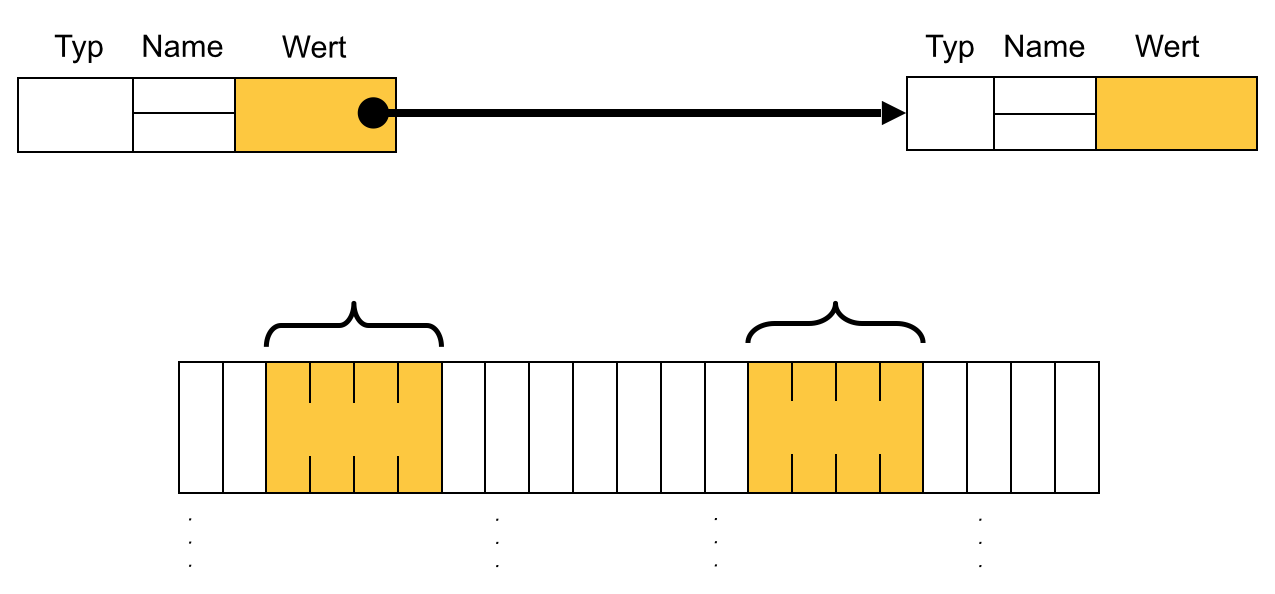
\includegraphics[width=.9\textwidth]{02_memory/figures/memory_image.png}
\end{center}

\hints{
	\item Die Speicheradressen kannst du frei wählen, der Pointer sollte aber natürlich auf die entsprechend gewählte Adresse zeigen.
}

\subsection{Bedeutung verstehen}
Versuche die Bedeutung folgender Ausdrücke zu verstehen.
Welche Regelmäßigkeiten stellst du fest?

\begin{minipage}{\linewidth}
\lstinputlisting{02_memory/problems/listings/pointers_intro_advanced.cpp}
\end{minipage}

\hints{
	\item Gehe dabei von rechts nach links vor.
}

\subsection{Gültigkeit}
Warum sind folgende Ausdrücke ungültig, sinnlos oder sogar gefährlich?

\vbox{ %fixes empty page
\lstinputlisting{02_memory/problems/listings/pointers_intro_validity.cpp}
}

\hints{
	\item Finde heraus, welchen Typ der Ausdruck hätte haben müssen.
	\item Nur tatsächlich angelegte Variablen haben Adressen. Ausdrücke wie a + b oder direkt kodierte Zahlenliterale wie 42 haben keine Adresse.
}

\subsection{Variablentausch}
Schreibe eine Funktion \lstinline{swap}, die zwei \lstinline{int}-Variablen miteinander vertauscht.
Probiere dabei beide möglichen Übergabevarianten (per Referenz, per Pointer) aus.
Was würde passieren, wenn man die Variablen stattdessen per Wert übergeben würde?

\subsection{Programmanalyse}
Sieh dir folgendes Programm an.

\vbox{ %fixes empty page
\lstinputlisting{02_memory/problems/listings/pointers_programm.cpp}
}

Welche Adressen werden übereinstimmen, welche werden sich unterscheiden?
Führe das Programm aus.
Hast du diese Ausgabe erwartet?

\subsection{Const Correctness}

In dieser Aufgabe setzt du dich mit der Bedeutung des Schlüsselworts \lstinline{const} im Kontext von Pointern auseinander.

Versuche für jede der Variablen im folgenden Code je eine \emph{Verwendung} zu finden, die  
\begin{itemize}
\item gültig ist (= fehlerfrei kompiliert) und
\item nicht gültig ist (= einen Compiler-Fehler wirft).
\end{itemize}


Was ist jeweils der Grund?
Welche Pointer verhalten sich gleich?

\lstinputlisting{02_memory/problems/listings/pointers_behavior.cpp}

\paragraph{Mehrstufige Pointer}

Versuche nun das Gleiche mit den folgenden mehrstufigen Pointern.

\lstinputlisting{02_memory/problems/listings/pointers_multi.cpp}

\subsection{Übergabewerte}
In der letzten Aufgabe direkt zu Pointern geht es darum, das gerade erlangte Verständnis über Pointer und Referenzen zu festigen und zu kontrollieren.
In Tabelle \ref{table:uebergabewerte} sind in der ersten Spalte Funktionen mit verschiedenen Parametern gegeben.
In der ersten Zeile findest du verschiedene Variablentypen.
Deine Aufgabe ist es nun, zu den verschiedenen Funktionen die passenden Parameter aus den Variablen herzustellen.
Falls eine Variable nicht ohne großartige Konversationen verwendet werden kann trage bitte ein \xmark ein. \\\\
Als Beispiel dient hierfür die erste Zeile. 

\begin{table}[h]
    \centering

    \newcolumntype{b}{X}
    \newcolumntype{s}{>{\hsize=.6\hsize}X}

    \begin{tabularx}{\textwidth}{b *5{| >{\centering\arraybackslash}s}@{}} 
		& \mbox{\lstinline!int i!} & \mbox{\lstinline!int *j!} & \mbox{\lstinline!int const *const k!} & \mbox{\lstinline!int **l!} & \mbox{\lstinline!const int *m!} \\ \hline
		\mbox{\lstinline!op1(int *)!}          & \mbox{\lstinline!&i!} & \mbox{\lstinline!j!} & \xmark & \mbox{\lstinline!*l!} & \xmark \\ \hline
		\mbox{\lstinline!op2(int)!}            & & & & & \\ \hline
		\mbox{\lstinline!op3(int &)!}         & & & & & \\ \hline
		\mbox{\lstinline!op4(const int **)!}   & & & & & 
    \end{tabularx}
    \caption{Tabelle für \emph{Übergabewerte} Aufgabe}
    \label{table:uebergabewerte}
\end{table}

\newpage
\section{Arrays und Zeigerarithmetik}
Arrays sind zusammenhängende Speicherbereiche, die mehrere Variablen von gleichem Typ speichern können.
Arrays werden in C++ folgendermaßen angelegt: \lstinline{<Typ> <name>[<Größe>];}, zum Beispiel:

\lstinputlisting{02_memory/problems/listings/arrays_intro.cpp}

Falls das Array global ist, muss die Größe eine konstante Zahl sein, falls das Array in einer Funktion auf dem Stack angelegt wurde, kann die Größe auch durch eine Variable vorgegeben werden.
Auf jeden Fall bleibt diese während der Existenz des Arrays konstant und kann sich nach dem Anlegen nicht mehr ändern.

Ein Array kann direkt bei der Deklaration initialisiert werden:

\lstinputlisting{02_memory/problems/listings/arrays_example.cpp}

Man kann die Größe optional auch weglassen, in diesem Fall wird sie der Compiler anhand der angegebenen Elemente selbst ermitteln.

Man kann auf die einzelnen Elemente des Arrays wie gewohnt über \textbf{arr[i]} zugreifen.

Arrays und Zeiger sind in C++ stark miteinander verwandt.
So ist der \textbf{Bezeichner} des Arrays gleichzeitig die \textbf{Adresse des ersten Elements}.
Somit kann man sowohl durch \textbf{*arr} als auch durch \textbf{arr[0]} auf das erste Element zugreifen.
Analog dazu kann man auch einen Zeiger auf das erste Element anlegen:

\lstinputlisting{02_memory/problems/listings/arrays_pointer.cpp}

Da die Elemente eines Array direkt hintereinander stehen, kann man den Zeiger inkrementieren, um zum  nächsten Element zu gelangen (sogenannte Pointerarithmetik).
Beispiel:

\lstinputlisting{02_memory/problems/listings/arrays_inc.cpp}

Somit kann man auf beliebige Elemente des Array über den Zeiger zugreifen:

\lstinputlisting{02_memory/problems/listings/arrays_pointer_inc.cpp}

Tatsächlich ist \textbf{*(p+i)} in \textbf{jeder Hinsicht äquivalent} zu \textbf{p[i]}.
Das bedeutet, dass man sowohl auf das i-te Element eines Arrays über \textbf{*(arr + i)} zugreifen kann als auch über \textbf{pointer[i]} auf das Element, auf welches der Zeiger \lstinline{pointer+i} zeigt!

In C++ findet keine automatische Bereichsprüfung bei Arrayzugriffen statt.
Du bist als Programmierer selbst dafür verantwortlich, dass niemals auf ein Element außerhalb der Array-Grenze zugegriffen wird.
Falls doch, kann es zu Programmabstürzen oder unerwünschten Effekten wie Buffer-Overflows kommen, die ein erhebliches Sicherheitsrisiko darstellen.
Bevorzuge deshalb Container-Klassen wie \lstinline{std::vector} (oder \lstinline{std::array} ab C++11) aus der Standardbibliothek anstelle von \glqq rohen\grqq{} Arrays.
Beachte außerdem, dass der \lstinline{delete[]}-Operator zwar das Array löscht, den Zeiger jedoch \textbf{nicht} auf \lstinline{NULL} setzt.
Dabei entsteht ein \emph{Dangling Pointer}, welcher dazu führen kann, dass später im Programm auf Speicherstellen zugegriffen wird, die nicht reserviert sind.
Setze deshalb Zeiger nach einem \lstinline{delete}/\lstinline{delete[]} sofort auf \lstinline{NULL}, um Speicherfehler zu vermeiden.

Um die Größe eines Arrays zu ermitteln, kannst du den \lstinline{sizeof()}-Operator benutzen.
Dieser gibt generell die Anzahl der Bytes an, die eine Variable verbraucht.
Da einzelne Array-Elemente größer als ein Byte sein können, muss die Gesamtgröße des Arrays durch die Größe eines Elements geteilt werden, um auf die Anzahl der Elemente zu kommen.

\lstinputlisting{02_memory/problems/listings/arrays_sizeof.cpp}

Beachte, dass \lstinline{sizeof()} \textbf{nicht} dazu verwendet werden kann, um die Größe des Arrays herauszufinden, auf die ein Zeiger zeigt.
In diesem Fall wird \lstinline{sizeof()} nämlich die \textbf{Größe des Zeigers} und nicht die Größe des Arrays liefern!

\lstinputlisting{02_memory/problems/listings/arrays_sizeof_pointer.cpp}

\subsection{Arrays anlegen}
Lege in der \lstinline{main}-Funktion ein \lstinline{int}-Array mit 10 Elementen an, und initialisiere es mit den Zahlen 1 bis 10.
Iteriere in einer Schleife über das Array und gib alle Elemente nacheinander aus.

\subsection{printElements implementieren}
In C und C++ kann man Arrays nicht direkt an Funktionen übergeben.
Stattdessen übergibt man einen Zeiger auf das erste Element des Arrays. Aufgrund der Äquivalenz von \textbf{*(p+i) } und \textbf{p[i]} kann man in der Funktion den Zeiger syntaktisch wie das Original-Array verwenden.

Schreibe eine Funktion, die einen \lstinline{const}-Zeiger auf das erste Element eines Arrays bekommt und alle Elemente ausgibt.
Da die Funktion nur anhand des Zeigers keine Möglichkeit hat zu wissen, wie groß das Array ist, muss die Größe des Arrays durch einen weiteren Parameter übergeben werden\footnote{Statt \lstinline{unsigned int} wird oft der Standard-Typ \lstinline{size_t} genutzt (z.B. in \lstinline{std::vector}).}:

\lstinputlisting{02_memory/problems/listings/arrays_printelems.cpp}

\subsection{Offset-basierte Ausgabe}
Wie wir vorher gesehen haben, kann man mit Zeigern auch rechnen und diese nachträglich ändern.
Anstatt mit einem Index das Array zu durchlaufen, kann man stattdessen bei jeder Iteration den Zeiger selbst inkrementieren!

\lstinputlisting{02_memory/problems/listings/arrays_iterate.cpp}

Schreibe die Funktion aus der vorherigen Aufgabe so um, dass sie einen laufenden Zeiger anstatt eines Indexes verwendet.

\subsection{Iterator-basierte Ausgabe}
Ebenso kann man auch die Arraygröße auf eine andere Weise übergeben, indem man die Adresse des Elements nach dem letzten Element angibt.
Dadurch werden Schleifen der folgenden Form möglich.

\lstinputlisting{02_memory/problems/listings/arrays_iterate_end.cpp}

möglich.
Schreibe die Funktion aus der vorherigen Aufgabe entsprechend um.
Vergiss nicht, den Zeiger als \lstinline{const} zu definieren, da Elemente nur gelesen werden.
Du kannst hier \lstinline{const} doppelt verwenden, um auch sicherzustellen, dass der \lstinline{end}-Zeiger nicht verändert wird.

\subsection{Subarrays ausgeben}
Die obige Methode, über Elemente eines Arrays zu iterieren, mag dir zunächst etwas ungewöhnlich erscheinen.
Sie hat jedoch den Vorteil, dass man anstatt des ganzen Arrays auch kleinere zusammenhängende Teile davon an Funktionen übergeben kann, indem man Zeiger auf die entsprechenden Anfangs-und Endelemente setzt.
Beispiel:

\lstinputlisting{02_memory/problems/listings/arrays_print_with_index.cpp}

Experimentiere etwas mit dieser Übergabemethode in deiner eigenen Funktion!

\subsection{Arrays auf dem Heap}
Bisher haben wir das Array auf dem Stack angelegt
Mit \textbf{new[]} kann man ein Array auf dem Heap erzeugen.
Dabei wird die Adresse des ersten Elements in einem Zeiger gespeichert.
Mittels \lstinline{delete[]} \textbf{muss} man den belegten Speicher nach Benutzung freigeben.
Beispiel:

\lstinputlisting{02_memory/problems/listings/arrays_heap.cpp}

Beachte die \textbf{[]} nach \lstinline{delete}.
Diese bewirken, dass das gesamte Array und nicht bloß das erste Element gelöscht wird.

Ein Anwendungsfall von dynamischen Arrays sind Funktionen, die ein Array von vorher unbekannter Größe zurückgeben.

Schreibe eine Funktion, die beliebig viele Zahlen von der Konsole mittels \lstinline{std::cin} einliest.
Der Benutzer soll dabei zuvor gefragt werden, wie viele Zahlen er eingeben möchte.
Speichere die Zahlen in einem dynamisch angelegten Array ab und lasse die Funktion einen Zeiger darauf zurückgeben.
Hier ist ein Beispiel wie \lstinline{std::cin} zu verwenden ist:

\lstinputlisting{02_memory/problems/listings/arrays_cin_size.cpp}

Zusätzlich zum Zeiger muss die Funktion auch die Möglichkeit haben, ihrem Aufrufer die Größe des angelegten Arrays mitzuteilen.
Füge der Funktion deshalb einen weiteren Parameter hinzu, in dem entweder per Referenz oder per Zeiger eine Variable übergeben wird, um dort die Größe abzulegen\footnote{Du merkst sicherlich schon jetzt, dass es umständlich/fehleranfällig ist, wenn man die Größe eines Arrays separat speichern und übergeben muss.}.

Gib die eingelesenen Werte auf der Konsole aus.
Vergiss nicht, am Ende den Speicher freizugeben.

\newpage
\section{Verkettete Listen}
In dieser Aufgabe wollen wir eine doppelt verkettete Liste von Integern implementieren.
Dazu brauchen wir zwei Klassen:
\lstinline{ListItem} stellt ein Element der Liste mit dessen Inhalt dar und \lstinline{List} speichert die Zeiger auf Anfangs- und Endelemente und bildet den eigentlichen Zugangspunkt für die Liste.

\begin{figure}[h]
\centering
\begin{tikzpicture}
    \def\blockdist{2}
    \def\captiondist{0.35}
    \tikzstyle{triple}=[rectangle split, rectangle split part fill={white, white, yellow}, thick, rectangle split parts=3, draw, align=center, text width=1.7cm]
    \tikzstyle{arrow}=[->, thick]

    % nodes
    \node (0) [triple] {next \nodepart{second}previous \nodepart{third} content};
    \path (0.east)+(\blockdist,0) node (1) [triple] {next \nodepart{second}previous \nodepart{third} content};
    \path (1.east)+(\blockdist,0) node (2) [triple] {next \nodepart{second}previous \nodepart{third} content};
    \path (2.east)+(\blockdist,0) node (3) [triple] {next \nodepart{second}previous \nodepart{third} content};
    \path (2.east)+(\blockdist,0) node (3) [triple] {next \nodepart{second}previous \nodepart{third} content};

    \coordinate (mid) at ($(1)!0.5!(2)$);
    \path (mid.south)+(0,-3) node (root) [triple, rectangle split part fill={white, white, white}] {first \nodepart{second}last \nodepart{third}currentSize};

    \path (0.west)+(-1.5,0) node (n1) {\textbf{NULL}};
    \path (3.25)+(1.5,0) node (n2) {\textbf{NULL}};

    % arrows
    \path[arrow] (0.25) edge (1.155);
    \path[arrow] (1.25) edge (2.155);
    \path[arrow] (2.25) edge (3.155);
    \path[arrow] (3.25) edge (n2.west);

    \path[arrow] (3) edge (2);
    \path[arrow] (2) edge (1);
    \path[arrow] (1) edge (0);
    \path[arrow] (0) edge (n1.east);

    \draw[arrow] (root.0) -| (3.south);
    \draw[arrow] (root.155) -| (0.south);

    % captions
    \path (0.north)+(0,\captiondist) node (c0) [] {\textbf{ListItem}};
    \path (1.north)+(0,\captiondist) node (c1) [] {\textbf{ListItem}};
    \path (2.north)+(0,\captiondist) node (c2) [] {\textbf{ListItem}};
    \path (3.north)+(0,\captiondist) node (c3) [] {\textbf{ListItem}};
    \path (root.north)+(0,\captiondist) node (croot) [] {\textbf{List}};
\end{tikzpicture}

\caption{Linked List}
\end{figure}

Wir werden am Tag 4 auf dieser Aufgabe aufbauen und die Liste um weitere Funktionen erweitern.
Behalte dies bitte im Hinterkopf und lösche deine Lösung nicht.
Falls du mit dieser Aufgabe bis dahin nicht fertig sein solltest, kannst du natürlich auch die Musterlösung als Ausgangspunkt nehmen.

\subsection{Klasse \lstinline{ListItem}}
Implementiere die Klasse \lstinline{ListItem}, welche die zu speichernde Zahl sowie Verweise auf das vorherige und nächste \lstinline{ListItem} als Attribute hat.
Verwende dazu Zeiger und keine Referenzen, da Referenzen nachträglich nicht mehr geändert werden können.
Auch können Referenzen nicht \lstinline{NULL} sein, was in unserem Fall nötig ist, um zu markieren, dass ein Element keine Vorgänger oder Nachfolger hat.

Der Konstruktor sollte sowohl seine eigenen \lstinline{next} und \lstinline{previous} Zeiger initialisieren, als auch die seiner Vorgänger- und Nachfolgerelemente.
Die Methode \lstinline{getContent()} soll eine Referenz auf den Inhalt zurückgeben, damit dieser durch eine Zuweisung modifiziert werden kann.

\begin{lstlisting}
class ListItem {
public:
	/**
	 * create a list item between two elements with a given given content
	 * (also modify previous->next and next->previous)
	 */
	ListItem(ListItem *prev, ListItem *next, int content);
	/**
	 * delete this list item (also change previous->next and next->previous
	 * to not point to this item anymore)
	 */
	~ListItem();				
	int & getContent();			// get a reference to the contained data
	ListItem * getNext();			// get the next list item or NULL
	ListItem * getPrevious();	// get the previous list item or NULL
private:
	ListItem *previous;		// previous item in list
	ListItem *next;			// next item in list
	int content;				// content of this list item
};
\end{lstlisting}

\subsection{Privater Copy-Konstruktor}
Unsere \lstinline{ListItem} Klasse hat einen kleinen Design-Fehler:
Da wir keinen Copy-Konstruktor definiert haben, generiert der Compiler automatisch einen.
Dieser kopiert einfach die einzelnen Attribute des Ursprungsobjekts (sogenannte ,,flache'' Kopie/Shallow Copy).
In unserem Fall ergibt das Kopieren eines \lstinline{ListItems} jedoch semantisch keinen Sinn, weil dabei ein hängendes \lstinline{ListItem} entstehen würde, welches nicht mit der Liste verknüpft ist, aber dennoch auf andere Items der Liste zeigt.

Deklariere in der Headerdatei einen \lstinline{private} Copy-Konstruktor und einen \lstinline{private} \lstinline{operator=}.
Dadurch können beide nie aufgerufen werden und der Kompiler kann dies zur Kompilierzeit überprüfen.

\begin{lstlisting}
private:
	ListItem(const ListItem &other);		// private copy constructor (without implementation)
	ListItem& operator=(const ListItem &other);	// private assignment operator (w/o implementation)
\end{lstlisting}

\hints{
	\item Alternativ kann man ab C++11 Funktionen explizit löschen:\\ 
    \lstinline{ListItem(const ListItem \&other) = delete;}\\
    \lstinline{ListItem\& operator=(const ListItem \&other) = delete;}
}

\subsection{Klasse \lstinline{List}}
Implementiere nun die Klasse \lstinline{List}.
Achte bei den Methoden zum Einfügen und Entfernen von Elementen darauf, dass bei einer leeren Liste eventuell sowohl die \lstinline{first} als auch \lstinline{last} Zeiger modifiziert werden müssen.
Vergiss nicht, \lstinline{currentSize} bei jeder Operation entsprechend anzupassen.
Falls die Liste leer ist, sollten \lstinline{deleteFirst()} und \lstinline{deleteLast()} einfach nichts ändern\footnote{Lieber würde man hier einen Fehler werfen, aber Exceptions haben wir an dieser Stelle noch nicht behandelt.}.

\paragraph{\lstinline{operator<<} implementieren}
Implementiere außerdem den \lstinline{operator<<}, um bequem Listen auf der Kommandozeile auszugeben.
Die übergebene Referenz ist -- entgegen der üblichen Konvention für \lstinline{operator<<} -- nicht \lstinline{const}, da wir ansonsten entsprechend eine \lstinline{const}-Version des  \lstinline{ListIterator} benötigen würden.

Vergiss hier nicht, \lstinline{operator<<} als \lstinline{friend} von \lstinline{List} zu deklarieren (wie zuvor bei \lstinline{Vector}).

\begin{lstlisting}
class List {
public:
	List();								// create an empty list
	~List();								// delete the list and all of its elements
	List(const List &other);		// create a copy of another list
	void appendElement(int i);		// append an element to the end of the list
	void prependElement(int i);	// prepend an element to the beginning of the list
	void insertElementAt(int i, int pos);	// insert an element i at position pos
	int getSize() const;				// get the number of elements in list
	int & getNthElement(int n);		// get content of the n-th element.
	int & getFirst();					// get content of the first element
	int & getLast();					// get content of the last element
	int deleteFirst();			// delete first element and return it (return 0 if empty)
	int deleteLast();				// delete last element and return it (return 0 if empty)
	int deleteAt(int pos);		// delete element at position pos
private:
	ListItem *first, *last;		// first and last item pointers (nullptr if list is empty)
	int currentSize;				// current size of the list
};

#include <iostream>

/** Print the given list to the stream. N.B. list should actually be const but then we would need const ListIterators */
std::ostream &operator<<(std::ostream &stream, List &list);
\end{lstlisting}

\subsection{Liste testen}
Teste deine Implementation.
Füge der Liste Elemente von beiden Seiten hinzu und lösche auch wieder welche.
Kopiere die Liste und gib die Elemente nacheinander aus.

\subsection{ListIterator}
Bisher haben wir über \lstinline{getNthElement()} auf die Elemente der Liste zugegriffen.
Diese Methode kann insbesondere bei langen Listen sehr langsam sein.
Deshalb werden wir einen Iterator schreiben, über den man auf die Listenelemente sequentiell zugreifen kann.
Der Iterator soll dabei einen Zeiger auf das aktuell betrachtete Element der Liste halten.

Um den Zugriff möglichst komfortabel zu gestalten, werden wir den Iterator als eine Art Zeiger implementieren, den man über \textbf{$++$} und \textbf{$--$} in der Liste verschieben kann.
Um auf ein Element zuzugreifen, überladen wir den Dereferenzierungsoperator \lstinline{operator*}.
Somit können wir unsere Liste ähnlich zu \lstinline{std::vector} verwenden:
\begin{lstlisting}
	for (ListIterator iter = list.begin(); iter != list.end(); iter++) {
		cout << *iter << endl;
	}
\end{lstlisting}

\paragraph{Konstruktor und Operatoren} 
Beginne mit einer Grundversion des Iterators.
Erstelle einen Konstruktor, der die Attribute des Iterators (Zeiger auf aktuelles Element und Zeiger auf die Liste) entsprechend initialisiert.
Implementiere Vergleichsoperator \lstinline{operator!=} sowie den Dereferenzierungsoperator \lstinline{operator*}.
Der Dereferenzierungsoperator solle den Inhalt des aktuellen Items zurückgeben.
Du brauchst nicht zu prüfen, ob \lstinline{item} tatsächlich auf ein gültiges Element zeigt (Das machen/können Iteratoren aus der Standardbibliothek übrigens auch nicht!).
Zum Vergleichen zweier Iteratoren prüfe, ob die \lstinline{item} und \lstinline{list} Zeiger identisch sind.
Vergleiche nicht den Inhalt der Items, da der Vergleich auch dann funktionieren soll, wenn \lstinline{item} \lstinline{NULL} ist, wenn der Iterator also auf kein Element zeigt.

\begin{lstlisting}
class ListIterator {
public:
	// create a new list iterator pointing to an item in a list
	ListIterator(List *list, ListItem *item);
	// get the content of the current element
	int& operator*();
	// check whether this iterator is not equal to another one
	bool operator!=(const ListIterator &other) const;
private:
	List *list;
	ListItem *item;
};
\end{lstlisting}


\paragraph{Zugriff von außen: ListIterator als friend-Klasse} Du wirst in den folgenden Methoden auf private Attribute von \lstinline{List} zugreifen müssen.
Um dies zu ermöglichen, könnte man öffentliche Getter für die Items der Liste schreiben.
Dadurch würde jedoch jeder die Möglichkeit bekommen, direkt auf die \lstinline{ListItem}s der Liste zuzugreifen, was dem Geheimnisprinzip zuwiderläuft.
Deshalb werden wir \lstinline{ListIterator} stattdessen explizit erlauben, auf \lstinline{private}-Attribute der Liste zuzugreifen.
Dazu müssen wir \lstinline{ListIterator} als \lstinline{friend} von \lstinline{List} deklarieren.
Füge dazu folgende Zeile (an beliebiger Stelle, üblich ist der Anfang der Klasse) zur Klassendefinition von \lstinline{List} hinzu:
\begin{lstlisting}
friend class ListIterator;
\end{lstlisting}

\paragraph{Iterator vorwärts bewegen mittels \lstinline{operator++}}

Implementiere den \lstinline{operator++} zum Inkrementieren des Iterators.
Falls der Iterator zuvor auf kein Item zeigte (\lstinline{item == NULL}), soll er nun auf das erste Element der Liste gesetzt werden.
Die Prototypen dazu lauten:
\begin{lstlisting}
ListIterator& operator++();		// increment this iterator and return itself (prefix ++)
ListIterator operator++(int);		// increment this iterator and return the previous (postfix ++)
\end{lstlisting}

Bei der Überladung des \lstinline{operator++} muss eine Sonderregelung beachtet werden.
Dieser Operator kann sowohl als Postfix (z.B. \lstinline{iter++}) als auch Präfix (z.B. \lstinline{++iter}) verwendet werden.
Um den Compiler darüber zu informieren, welche Variante wir überladen, wird beim Postfix-Operator ein Dummy-Parameter vom Typ \lstinline{int} definiert.
Dieser dient nur der syntaktischen Unterscheidung und hat keine weitere Bedeutung.

Beachte außerdem, dass bei Präfix-Operationen der Iterator sich selbst zurückgeben sollte, während der Postfix-Operationen eine Kopie des Iterators zurückgibt, die auf das vorherige Element zeigt.
Das ist auch der Grund, warum die Präfix-Form von \lstinline{operator++} (und \lstinline{operator--}) effizienter ist als die Postfix-Form.
Daher sollte die Präfix-Form dieser Operatoren die bevorzugte Variante sein, falls kein besonderer Grund für die Postfix-Form vorliegt.

Zum besseren Verständnis ist ein Teil der Implementation gegeben:

\begin{lstlisting}
// Prefix ++  ->  increment iterator and return it
ListIterator& ListIterator::operator++() {
	if (item == NULL) {
		item = ...	 // set item to first item of list
	}
	else {
		item = ...	 // set item to next item of current item
	}
	return *this;	 // return itself
}

// Postfix ++  -> return iterator to current item and increment this iterator
ListIterator ListIterator::operator++(int) {
	ListIterator iter(list, item); // Store current iterator
	if (item == NULL) {
		item = ...	 // set item to first item of list
	}
	else {
		item = ...	 // set item to next item of current item
	}
	return iter; 	// return iterator to previous item
}
\end{lstlisting}


\paragraph{Iterator rückwärts bewegen mittels \lstinline{operator--}}
Überlade auf die gleiche Weise auch den \lstinline{operator--} sowohl in Postfix als auch Präfix-Form.

\paragraph{Iteratoren in List erzeugen} 
Nun ist unsere Implementation fast komplett und wir brauchen nur noch Methoden, um Iteratoren zu erzeugen.
Implementiere dazu die folgenden Methoden innerhalb der \lstinline{List} Klasse, um Iteratoren auf das erste und letzte Element der Liste zu erzeugen.
\begin{lstlisting}
ListIterator begin();		// return an iterator pointing to the first element
ListIterator end();			// return an iterator pointing to the element after the last one
\end{lstlisting}

Höchstwahrscheinlich wirst du Probleme bei der Kompilierung haben.
Dies liegt an der zirkulären Abhängigkeit zwischen \lstinline{List} und \lstinline{ListIterator}.
Gehe dazu folgendermaßen vor:
Verschieben die \lstinline{\#include} Anweisungen für die Header von \lstinline{List} und \lstinline{ListItem} aus \filename{ListIterator.h} nach \filename{ListIterator.cpp} und füge in \filename{ListIterator.h} folgendes hinzu

\begin{lstlisting}
class ListItem;
class List;
\end{lstlisting}

Dies sind Vorwärtsdeklarationen (\textbf{Forward Declaration}), die dem Compiler sagen, dass die Klassen existieren, aber später definiert werden. Nun kannst problemlos \filename{ListIterator.h} in \filename{List.h} einbinden.

\subsection{Liste mit ListIterator testen}
Teste deine Implementation.
Erstelle eine Liste, füge Elemente hinzu und iteriere über Listenelemente:

\begin{lstlisting}
for (ListIterator iter = list.begin(); iter != list.end(); iter++) {
	cout << *iter << endl;
}
\end{lstlisting}

Warum kann man \textbf{nicht} rückwärts durch die Liste iterieren, indem man einfach die Aufrufe \lstinline{list.begin()} und \lstinline{list.end()} tauscht und \lstinline{iter--} statt \lstinline{iter++} verwendet?
Denke daran, worauf die von \lstinline{begin()} und \lstinline{end()} zurückgegebenen Iteratoren zeigen.

\hints{
	\item In der Standardbibliothek gibt es hierfür \lstinline{rbegin()} und \lstinline{rend()}
}

\newpage
\section{Exceptions}
Ähnlich wie in Java können Fehler während der Programmlaufzeit in C++ mittels Exceptions signalisiert werden.

\lstinputlisting{problems/listings/exceptions_intro.cpp}

Es gibt jedoch einige Unterschiede zur Fehlerbehandlung in Java.
Das aus Java bekannte \lstinline{finally}-Konstrukt existiert in C++ nicht.
Außerdem kann jede Art von Wert geworfen werden -- sowohl Objekte als auch primitive Werte wie z.B. \lstinline{int}.
In der Praxis wird es jedoch empfohlen, den geworfenen Wert von \lstinline{std::exception} abzuleiten oder eine der existierenden Klassen aus der Standardbibliothek zu nutzen.

Im Gegensatz zu Java kann man Objekte nicht nur \emph{by-Reference} sondern auch \emph{by-Value} werfen und fangen.
In diesem Fall wird das geworfene Objekt nach der Behandlung im \lstinline{catch}-Block automatisch zerstört.
Wenn es \emph{by-Value} gefangen wird, wird das geworfene Objekt kopiert, ähnlich wie bei einem Funktionsaufruf.
Beispiel:

\lstinputlisting{problems/listings/exceptions_by_what.cpp}

In der Praxis hat es sich durchgesetzt, \emph{by-Value} zu werfen und \emph{by-const-Reference} zu fangen.

\subsection{Implementierung einer Dummy-Klasse}
Erstelle eine Klasse \lstinline{C} und implementiere einen Konstruktor, einen Copy-Konstruktor und einen Destruktor.
Versehe diese mit Ausgaben auf der Konsole, so dass der Lebenszyklus während der Ausführung ersichtlich wird.

\subsection{}
Experimentiere mit Exceptions.
Probiere insbesondere die beiden o.g. Fälle aus und beobachte die Ausgabe.
Wann wird ein Objekt erstellt/kopiert/gelöscht?
Teste auch, was passiert, wenn du mehrere \lstinline{catch}-Blöcke erstellst und sich diese nur in der Übergabe unterscheiden (Wert/Referenz).

\lstinputlisting{problems/listings/exceptions_multiple_catch.cpp}

Welcher \lstinline{catch} Block wird aufgerufen?
Spielt die Reihenfolge eine Rolle?

\subsection{Erweitern der Klasse \lstinline{List}}
Füge der Klasse \lstinline{List} vom Vortag Bereichsprüfungen hinzu.
Schreibe die Methoden \lstinline{insertElementAt()}, \lstinline{getNthElement()} und \lstinline{deleteAt()} so um, dass eine Exception geworfen wird, falls der angegebene Index die Größe der Liste überschreitet.
Verwende als Exception die Klasse \lstinline{std::out_of_range}\footnote{\url{http://en.cppreference.com/w/cpp/error/out_of_range}} aus dem \lstinline{stdexcept} Header.

\hints{
    \item Du musst hierbei keinerlei \lstinline{catch} Block verwenden, da es rein um das werfen einer Exception geht.
}

\subsection{Testen der Implementierung}
Teste die erweiterte Implementierung der Klasse List.
Provoziere eine Exception, indem du falsche Indices angibst, und fange die Exception als \lstinline{const} Referenz mit einem \lstinline{catch} Block ab (s.o.).
Du kannst die Methode \lstinline{what()}\footnote{\url{http://en.cppreference.com/w/cpp/error/exception/what}} benutzen, um an den Nachrichtentext der Exception zu gelangen.

\newpage
\section{Smart Pointers}
In dieser Aufgabe werden wir uns mit der Benutzung von Smart Pointers vertraut machen. Dazu werden wir die Smart Pointer Klassen \texttt{boost::shared\_ptr} und \texttt{boost::weak\_ptr} der Boost-Bibliothek verwenden.

\subsection{}
Erstellen eine Klasse \texttt{TreeNode}, die einen Knoten eines Binärbaums darstellt.
Jeder Knoten hat einen Inhalt vom Typ \texttt{int} sowie einen Zeiger auf seine beiden Kindknoten.
Statt \glqq roher\grqq{} Zeiger verwenden wir Smart Pointers, die das Speichermanagement übernehmen.
Dadurch wird es nicht nötig sein, Kindknoten manuell zu löschen.
Sie werden automatisch entfernt, sobald der Wurzelknoten gelöscht ist und keine Zeiger mehr auf den Kindknoten zeigen.

\begin{lstlisting}
#include <boost/shared_ptr.hpp>
class TreeNode;

typedef boost::shared_ptr<TreeNode> TreeNodePtr;	// typedef for better reading

class TreeNode {
public:
	/** create a new tree node and makes it shared */
	static TreeNodePtr createNode(int content, TreeNodePtr left = TreeNodePtr(), TreeNodePtr right = TreeNodePtr());
	~TreeNode();
private:
	TreeNode(int content, TreeNodePtr left, TreeNodePtr right);	// create a tree node
	TreeNodePtr leftChild, rightChild;									// left and right child
	int content;																// node content
};
\end{lstlisting}

Der Konstruktor von \texttt{TreeNode} privat, weil nur die Smart Pointer die Verantwortung für die Lebenszeit eines Objektes übernehmen sollen und bestimmen, wann es gelöscht wird.
Würde man \texttt{TreeNode}-Objekte direkt auf dem Stack anlegen, kann es passieren, dass der Objektdestruktor mehrmals aufgerufen wird -- einmal vom Smart Pointer und einmal beim Verlassen der Funktion.
Ebenso sollten wir keine Rohzeiger auf das Objekt erzeugen, da diese das Speichermanagement der Smart Pointer umgehen.
Stattdessen stellen wir eine statische Methode bereit, um \texttt{TreeNode}-Objekte auf dem Heap zu erzeugen und diese direkt einem Smart Pointer zu übergeben.

Implementiere den Konstruktor, Destruktor sowie \texttt{createNode}.
Der Konstruktor sollte die Attribute entsprechend initialisieren.
Schreibe auch eine Textausgabe, die den Zeitpunkt der Erzeugung eines \texttt{TreeNode}s deutlich macht.
Der Destruktor braucht die Kindknoten nicht zu löschen, da dies bei der Zerstörung des Elternknotens automatisch geschieht.
Füge auch hier eine Textausgabe ein, die die Zerstörung des Objekts sichtbar macht.

Das Schlüsselwort \textbf{static} sowie die Default-Parameter müssen bei der Implementation der Methode ausgelassen werden.
Der Smart Pointer für die Rückgabe wird mit einem Zeiger auf ein \texttt{TreeNode}-Objekt initialisiert. Somit lautet der Methodenrumpf

\begin{lstlisting}
TreeNodePtr TreeNode::createNode(int content, TreeNodePtr left, TreeNodePtr right) {
	return TreeNodePtr(new TreeNode(...));
}
\end{lstlisting}

\subsection{}
Teste, ob die einzelnen Knoten tatsächlich gelöscht werden, sobald kein Zeiger mehr auf den Elternknoten zeigt.
Erstelle dafür einen kleinen Baum:

\begin{lstlisting}
TreeNodePtr node = TreeNode::createNode(1, TreeNode::createNode(2), TreeNode::createNode(3));
\end{lstlisting}

Führe das Programm aus und beobachte die Ausgabe.
Sobald \texttt{main} verlassen wird, wird der Zeiger \texttt{node} gelöscht, und somit auch das dahinterliegende \texttt{TreeNode}-Objekt mit all seinen Kindknoten.

Um ganz sicher zu gehen, dass der Baum tatsächlich beim Löschen des letzten Zeigers zerstört wurde und nicht etwa durch das Beenden des Programms, kannst du \texttt{node} mit einem anderen Baum überschreiben.
Füge in diesem Fall am Ende des Programms eine Textausgabe hinzu, damit ersichtlich wird, dass der erste Baum noch vor Verlassen der \texttt{main} gelöscht wurde.

\subsection{}
Nun wollen wir \texttt{TreeNode} so erweitern, dass jeder Knoten Kenntnisse über seinen Elternknoten besitzt.
Füge das Attribut

\begin{lstlisting}
	TreeNodePtr parent;		// parent node
\end{lstlisting}

hinzu.
Da der Elternknoten beim Erzeugen eines \texttt{TreeNode}s undefiniert ist, brauchst du den Konstruktor nicht zu ändern. \texttt{parent} wird dann automatisch mit NULL initialisiert.

Implementiere die folgende Methode, die einem Knoten seinen Elternknoten zuweist:

\begin{lstlisting}
	void setParent(const TreeNodePtr &p);		// set parent of this node
\end{lstlisting}

\emph{Hinweis}:
\texttt{p} wird in diesem Fall nur deshalb als \texttt{const} Referenz übergeben, da es verhältnismäßig aufwändig ist, einen Smart Pointer zu kopieren.
Beachte, dass im obigen Fall der Smart Pointer selbst const ist, und nicht das Objekt, worauf er zeigt.

Jetzt muss noch \texttt{createNode()} modifiziert werden, sodass \texttt{setParent()} auf den Kindknoten aufgerufen wird. Da ein Smart Pointer die Operatoren $*$ und $->$ überladen hat, lässt er sich syntaktisch wie ein normaler Zeiger benutzen. Um zu überprüfen, ob ein Smart Pointer auf ein Objekt zeigt, kann dieser implizit nach \texttt{bool} gecastet werden. Somit lautet die neue Implementation von \texttt{createNode()}:

\begin{lstlisting}
TreeNodePtr TreeNode::createNode(int content, TreeNodePtr left, TreeNodePtr right) {
	TreeNodePtr node(new TreeNode(content, left, right));
	if (left) {
		left-> ... ; // set parent node
	}
	if (right) {
		right-> ... ; // set parent node
	}
	return node;
}
\end{lstlisting}

\subsection{}
Teste deine Implementation.
Du brauchst dazu in \texttt{main} nichts zu ändern.

Erschreckenderweise siehst du nun, dass überhaupt keine \texttt{TreeNode}-Objekte mehr gelöscht werden.
Die Ursache dafür ist die zirkuläre Abhängigkeit zwischen Kind- und Elternknoten.
Denn selbst wenn sie keine Zeiger auf den Wurzelknoten eines Baumes haben, verweisen die Kindknoten noch immer darauf.

Um dieses Problem zu lösen, müssen die Verweise zum Elternknoten \emph{schwach} (weak) sein.
Ein Knoten darf gelöscht werden, wenn nur noch schwache Zeiger (oder keine) auf ihn verweisen.
Binde dazu den Header \texttt{boost/weak\_ptr.hpp} ein und erstelle ein neues \texttt{typedef} für einen schwachen \texttt{TreeNode} Smart Pointer:

\begin{lstlisting}
typedef boost::weak_ptr<TreeNode> TreeNodeWeakPtr;
\end{lstlisting}

Ändere nun den Typ von \texttt{parent} auf \texttt{TreeNodeWeakPtr}.
Es müssen keine weiteren Änderungen gemacht werden, da starke Zeiger (\texttt{shared\_ptr}) implizit in schwache Zeiger (\texttt{weak\_ptr}) umgewandelt werden können.

\subsection{}
Teste deine Implementation.
Nun sollte sich \texttt{TreeNode} wie gewünscht verhalten.


\newpage
\setHeader{Aufgaben zur Objektorientierung in C++}
\section{\ExercisePrefixObjectOrientation Vererbung und Polymorphie}\label{sec:inheritance}
\cpppSolutionName{inheritance_polymorphism}{in\-heri\-tance\_poly\-morphism}
In dieser Aufgabe sollst du Konzepte der Vererbung und Polymorphie unter Verwendung abstrakter Funktionen erlernen.

\subsection{Klasse \lstinline{Person}}
Implementiere eine Klasse \lstinline{Person}, die eine Person mit einem Namen darstellt.
Füge allen Konstruktoren und Destruktoren eine Ausgabe auf die Konsole hinzu, um später den Lebenszyklus der Objekte besser nachvollziehen zu können.

\cpppInputListing{03_oo/problems/listings/inheritance_person.hpp}

\hints{
    \item Verwende \lstinline{\#include <string>} um \lstinline{std::string} zu verwenden.
    \item Um ein String-Literal an eine \lstinline{std::string} Variable anzuhängen, musst du aus dem String-Literal zuerst ein \lstinline{std::string}-Objekt machen: \lstinline{std::string text = std::string("Name: " ) + name;}.
}

\subsection{Klasse \lstinline{Student}}
Implementiere eine Klasse \lstinline{Student}, die von \lstinline{Person} erbt (\lstinline{public}) und einen Studenten mit einer Matrikelnummer (ebenfalls \lstinline{std::string}) modelliert.
Rufe in der Initialisierungsliste den entsprechenden Konstruktor der Elternklasse \lstinline{Person} mittels \lstinline{Person(name)} auf.
Füge allen Konstruktoren und Destruktoren eine Ausgabe auf die Konsole hinzu, um später den Lebenszyklus der Objekte besser nachvollziehen zu können.

\cpppInputListing{03_oo/problems/listings/inheritance_student.hpp}

\hints{
    \item Du kannst bei Bedarf die \lstinline{getInfo()}-Implementation der Elternklasse \lstinline{Person} von \lstinline{Student} aus mittels \lstinline{Person::getInfo()} aufrufen.
}

\subsection{Test}
Erstelle nun in \lstinline{main()} je eine Person und einen Studenten und gib deren Daten auf der Konsole aus.
Vergewissere dich, dass bei \lstinline{Student} auch die Matrikelnummer ausgegeben wird.
Schau dir auch die Ausgaben der Konstruktoren und Destruktoren an, und versuche, diese nachzuvollziehen.

Implementiere dann folgende Funktion und teste deine Implementation erneut, indem du \lstinline{printPersonInfo()} mit beiden Personentypen aufrufst.

\cpppInputListing{03_oo/problems/listings/inheritance_person_info.hpp}

\hints{
    \item Dadurch dass \lstinline{Person} als \lstinline{const} Zeiger übergeben wird, können auch Unterklassen von \lstinline{Person}, wie z.B. \lstinline{Student}, übergeben werden. 
}


\subsection{Dynamic Dispatch bei \lstinline{printPersonInfo}}
Du merkst, dass \lstinline{printPersonInfo()} unabhängig von übergebenem Typ einer Person immer nur den Namen der Person ausgibt, aber nicht die Matrikelnummer.
Der Grund dafür ist, dass \lstinline{getInfo()} nicht als \lstinline{virtual} deklariert wurde und deshalb auch kein dynamischer Dispatch der Methode stattfindet.
Deklariere daher \lstinline{getInfo()} in beiden Klassen als \lstinline{virtual}.

Teste deine Implementation erneut und vergewissere dich, dass nun immer die richtige Methode aufgerufen wird.

\hints{
	\item Möchte man Methoden einer Basisklasse überschreiben, \textbf{muss} \lstinline{virtual} in der Basisklasse gesetzt werden.
	In den abgeleiteten Klassen kann \lstinline{virtual} weggelassen werden, es wird dann vom Compiler ergänzt.
	Es ist aber hilfreich, auch dort der Lesbarkeit halber das Schlüsselwort zu verwenden.
	\item Erst ab C++11 gibt es die Möglichkeit mit dem Schlüsselwort \lstinline{override} zu deklarieren, dass eine Funktion eine andere (virtuelle) überschreibt (vergleichbar mit der Annotation \lstinline{@Override} in Java).
}

\subsection{Virtueller Destruktor}
Lege einen Studenten mit \lstinline{new} dynamisch auf dem Heap an und speichere die Adresse in einem Zeiger auf eine \lstinline{Person}.
Lösche die Person anschließend mit \lstinline{delete}.

\cpppInputListing{03_oo/problems/listings/inheritance_main.cpp}

Analysiere die Konsolenausgabe.
Es wird nur der Destruktor von \lstinline{Person} aufgerufen, obwohl es sich um ein Objekt vom Typ \lstinline{Student} handelt.
Auch hier liegt es daran, dass kein dynamischer Dispatch bei der Zerstörung erfolgt.
Deklariere deshalb in beiden Klassen den Destruktor als \textbf{virtual} und teste die Korrektheit der Destruktoraufrufe.

\hints{
    \item Faustregel: Besitzt eine Klasse mindestens eine virtuelle Funktion, so sollte auch der Destruktor virtuell sein.
}

\newpage
\section{Pure Virtual}
In dieser Aufgabe wollen wir Vererbung und Polymorphie dazu nutzen, um mathematische Ausdrücke als Bäume von Primitivoperationen zu modellieren.
Dazu werden wir eine abstrakte Oberklasse \texttt{Expression} mit der abstrakten Methode \texttt{compute()} erstellen.
Einzelne Knotentypen wie Addition und Subtraktion werden von \texttt{Expression} abgeleitet und implementieren \texttt{compute()}, um die jeweilige Operation zu realisieren.
\begin{figure}[h]
\begin{center}
	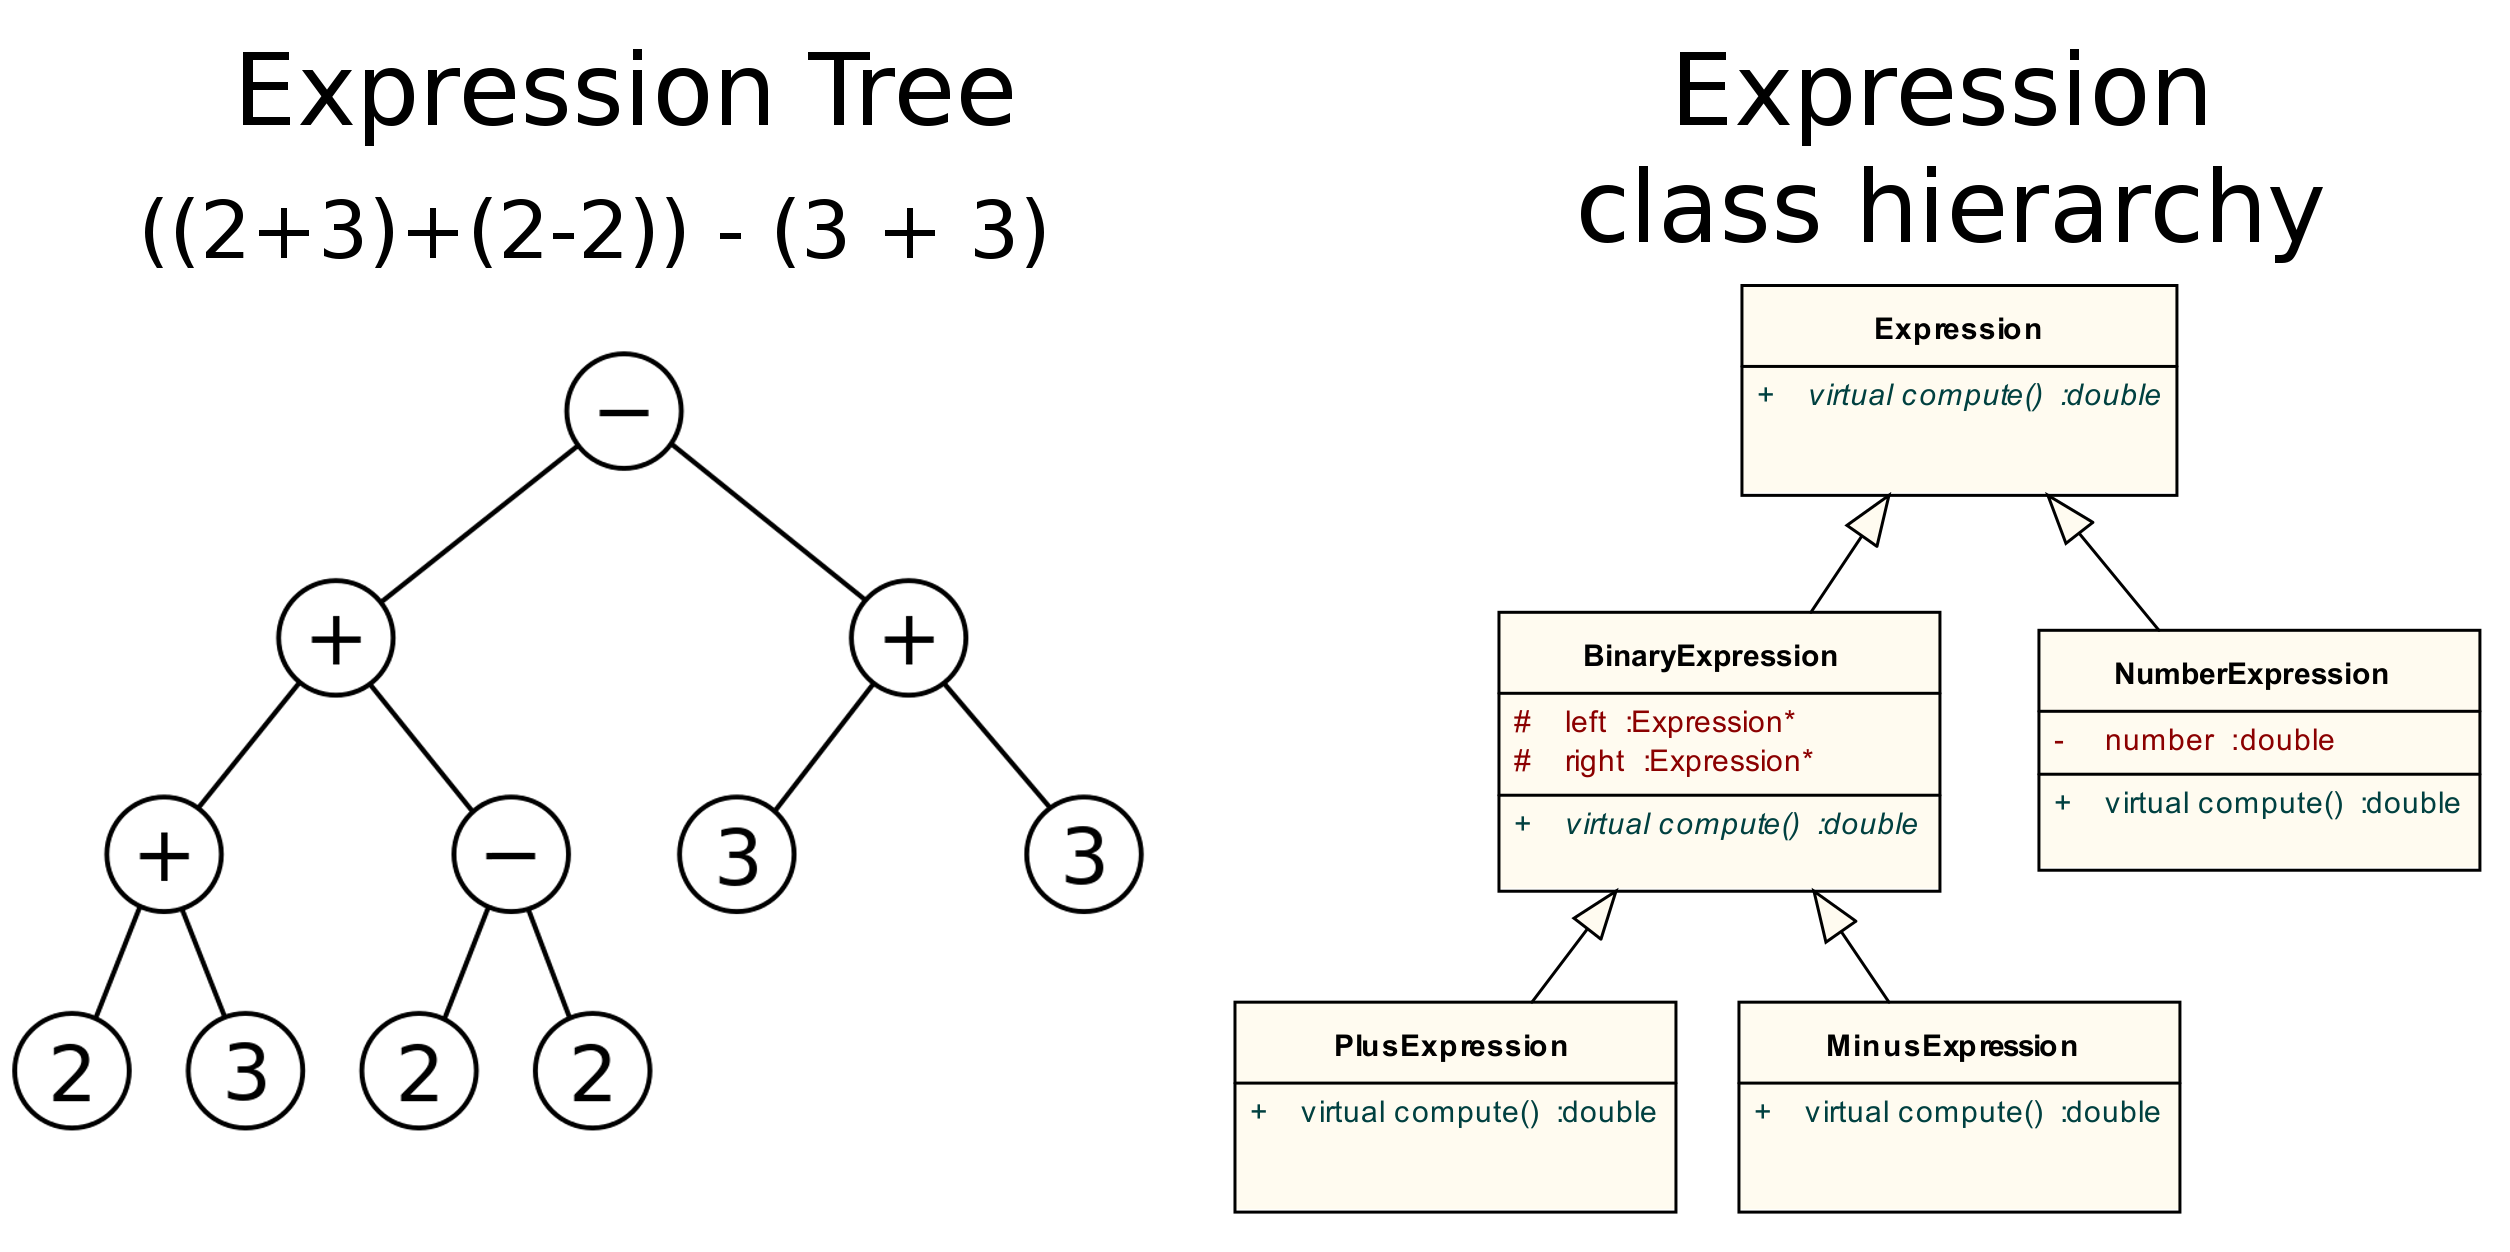
\includegraphics[width=.75\textwidth]{figures/ExpressionTree.png}\\
	\caption{Abbildung: Beispielausdruck mit Ausdrucksbaum und Klassenhierarchie}
\end{center}
\end{figure}


\begin{enumerate}

\item \textbf{Klasse \texttt{Expression}:}
Schreibe die abstrakte Klasse \texttt{Expression}.
Diese soll als Basisklasse für alle Ausdrücke dienen.
Implementiere einen parameterlosen Konstruktor und einen virtuellen Destruktor, die je eine Meldung auf der Konsole ausgeben, sodass es bei der Ausführung ersichtlich wird, wann eine \texttt{Expression} erzeugt und wann zerstört wird.
Deklariere außerdem eine abstrakte (pure \texttt{virtual}) Methode \texttt{virtual double compute() = 0;}, die das Ergebnis des Ausdrucks berechnen und zurückgeben soll. 

\item \textbf{Klasse \texttt{NumberExpression}:}
Schreibe die Klasse \texttt{NumberExpression}, die ein (Baum-)Blatt mit einer Zahl darstellt.
Dementsprechend soll \texttt{NumberExpression} von \texttt{Expression} erben und ein Attribut zum Speichern einer Zahl besitzen, das im Konstruktor initialisiert wird.
Implementiere den Konstruktor und virtuellen Destruktor und versehe auch diese mit einer Konsolenausgabe.
Die Methode \texttt{compute()} gibt die gespeicherte Zahl zurück.

\item \textbf{Klasse \texttt{BinaryExpression}:}
Schreibe die abstrakte Klasse \texttt{BinaryExpression} mit den \texttt{protected} Attributen \texttt{Expression *left, *right}.
Implementiere den Konstruktor und virtuellen Destruktor mit entsprechender Ausgabe.

\item \textbf{Klassen \texttt{PlusExpression} und \texttt{MinusExpression}:}
Schreibe die Klassen \texttt{PlusExpression} und \texttt{MinusExpression}, die von \texttt{BinaryExpression} erben und eine Addition bzw. Subtraktion realisieren. 
Implementiere die Kon- und Destruktoren sowie die \texttt{compute()} Methode.

\item \textbf{Testlauf:}
Teste deine Implementation.
Ein gutes Beispiel findest du in Abbildung weiter oben.
Schaue dir die Ausgabe genau an und versuche anhand der gegebenen Klassenhierarchie die Reihenfolge der Erzeugung und Zerstörung von Objekten  nachzuvollziehen.

\end{enumerate}

\newpage
\section{Mehrfachvererbung}
Nimm dir als Basis für diese Aufgabe die 1.\,Aufgabe aus der gestrigen Übung.

\subsection{Klasse \texttt{Employee}}
Schreibe die Klasse \texttt{Employee}, die einen Mitarbeiter darstellt.
\texttt{Employee} soll von \texttt{Person} erben und den Namen seines Vorgesetzten als Attribut beinhalten.
Erweitere auch entsprechend die Methode \texttt{getInfo()}.

\subsection{Klasse \texttt{StudentAssistant}}
Schreibe nun eine Klasse \texttt{StudentAssistant}, die eine wissenschaftliche Hilfskraft modelliert.
Eine wissenschaftliche Hilfskraft ist ein Student und gleichzeitig auch ein Mitarbeiter.
Dementsprechend soll \texttt{StudentAssistant} sowohl von \texttt{Student} als auch von \texttt{Employee} erben. Das heißt es werden je ein Student- und ein Employee-Objekt im Konstruktor initialisiert.
Weitere Attribute sind nicht nötig.
Überschreibe \texttt{getInfo()}, um alle Daten auszugeben.
Ändere dazu die Sichtbarkeit der Attribute sowohl von \texttt{Student} als auch von \texttt{Employee} von \texttt{private} auf \texttt{protected}.

Du wirst feststellen, dass sich die Klasse nicht kompilieren lässt, falls du das Attribut \texttt{name} direkt verwendest, da in einer \texttt{StudentAssistant}-Instanz zwei Instanzen von \texttt{Person} vorhanden sind - je eine von jeder Elternklasse. Deshalb müsse mittels dem Scope-Operator $::$ angeben, welche Basis du genau meinst.
\begin{lstlisting}
Employee::name
// or
Student::name
\end{lstlisting}

Teste deine Implementation, indem du das Ergebnis von \texttt{getInfo()} direkt in der \texttt{main} ausgibst.

\subsection{Virtuelle Vererbung}
Versuche nun, \texttt{printPersonInfo()} mit einer Instanz von \texttt{StudentAssistant} aufzurufen. Auch hier wird der Compiler mit einer Fehlermeldung abbrechen, da er nicht weiß, welche der beiden Basisklassen er nehmen soll.
Diesmal ist es in C++ allerdings nicht mehr möglich, die Basisklasse zu spezifizieren, weshalb wir anders vorgehen werden.
Wir sorgen mittels virtueller Vererbung dafür, dass \texttt{Person} nur ein Mal in \texttt{StudentAssistant} vorhanden ist.

Lasse dazu \texttt{Student} und \texttt{Employee} virtuell von \texttt{Person} erben.
Noch lässt sich das Programm nicht kompilieren, denn sowohl \texttt{Student} als auch \texttt{Employee} versuchen, einen Konstruktor von \texttt{Person} aufzurufen.
Da \texttt{Person} aber nur ein einziges mal in \texttt{StudentAssistant} vorhanden ist, müsste der Konstruktor demnach zwei mal aufgerufen werden -- einmal von \texttt{Student} und einmal von \texttt{Employee}.
Dies würde jedoch grob gegen die Sprachprinzipien verstoßen.
Deshalb wird der Konstruktor von \texttt{Person} weder von \texttt{Student} noch von \texttt{Employee} aufgerufen!
Stattdessen müssen wir in der Initialisierungsliste von \texttt{StudentAssistant} angeben, welcher Konstruktor von \texttt{Person} aufgerufen werden soll.
Die Konstruktoraufrufe innerhalb von \texttt{Student} und \texttt{Employee} laufen stattdessen ins Leere, auch wenn sie syntaktisch vorhanden sind! Füge deshalb ein \texttt{Person(name)} in die Initialisierungsliste von \texttt{StudentAssistant} hinzu.

Teste deine Implementation.
Versuche auch Folgendes: Ändere die Namen in den Konstruktoraufrufen von \texttt{Student} und \texttt{Employee} in der Initialisierungsliste von \texttt{StudentAssistant} und beobachte die Ausgabe.
Mache dir dadurch klar, welche Probleme Mehrfachvererbung von implementierten Klassen verursachen kann!

\subsection{Erklärung}

Eine Alternative zur Implementationsvererbung stellt \textbf{Schnittstellenvererbung} dar, wie es in Java üblich ist. Dabei werden Schnittstellen (Klassen mit ausschließlich abstrakten Methoden und ohne Attribute) definiert und nur diese vererbt.
Zusätzlich gibt es Implementationen von diesen Schnittstellen.
Man würde also \texttt{Person}, \texttt{Student}, \texttt{Employee} und \texttt{StudentAssistant} in jeweils zwei Klassen aufteilen, eine Schnittstelle und eine Implementation.
Die Schnittstellen würden voneinander erben, z.B. \texttt{StudentBase} von \texttt{PersonBase}, und entsprechende pur virtuelle/abstrakte Methoden wie \texttt{virtual std::string StudentBase::GetStudentID() = 0} bereitstellen.
Die Implementation würde ausschließlich von der jeweiligen Schnittstelle erben (\texttt{Student} von \texttt{StudentBase}).
Diese Variante erscheint zwar aufwändiger als Implementationsvererbung, vermeidet aber viele der dabei entstehenden Probleme.
Schnittstellenvererbung kann in Java eingesetzt werden, um Mehrfachvererbung zu realisieren.



\newpage
\setHeader{Aufgaben zu fortgeschrittenen Themen in C++}
\section{Template Funktionen}
\subsection{Templatefunktionen implementieren}
Implementiere die folgende Funktion, die das Maximum von zwei Variablen liefert:

\begin{lstlisting}
template<typename T>
const T &maximum(const T &t1, const T &t2);
\end{lstlisting}

Durch die Verwendung von Templates soll die Funktion mit verschiedenen Datentypen funktionieren.
Teste deine Implementation.

In der Vorlesung haben wir gesehen, dass jede Verwendung von \texttt{t1} und \texttt{t2} in \texttt{maximum} eine Schnittstelle induziert, die der Typ \texttt{T} bereitstellen muss.
Das bedeutet, dass \texttt{T} alle Konstruktoren, Methoden und Operatoren zur Verfügung stellen muss, die in \texttt{maximum} genutzt werden.

Wie sieht diese Schnittstelle in diesem Fall aus?

\hints{
    \item Anstelle von \texttt{typename} kann auch \texttt{class} in der Template-Deklaration verwendet werden.
}

\subsection{Explizite Angabe der Typparameter}
Lege nun zwei Variablen vom Typ \texttt{int} und \texttt{short} an, und versuche, mittels \texttt{maximum()} das Maximum zu bestimmen.
Der Compiler wird mit der Fehlermeldung \textbf{no matching function for call...} abbrechen, da er nicht weiß, ob \texttt{int} oder \texttt{short} der Template-Parameter sein soll.
Gib deshalb den Template-Parameter mittels \texttt{maximum<int>()} beim Aufruf von \texttt{maximum()} explizit an.
Die übergebenen Parameter werden dabei vom Compiler automatisch in den gewünschten Typ umgewandelt.

\subsection{Induzierte Schnittstelle implementieren}
Erstelle eine Klasse \texttt{C}, die eine Zahl als Attribut beinhaltet. Implementiere einen passenden Konstruktor sowie einen Getter für diese Zahl. Nun wollen wir unsere Funktion  \texttt{maximum()} verwenden, um zu entscheiden, welches von zwei \texttt{C}-Objekten die größere Zahl beinhaltet.
Überlege dir, was zu tun ist, und implementiere es.

\hints{
	\item Die Klasse \texttt{C} muss mindestens die durch \texttt{maximum} induzierte Schnittstelle implementieren.
}

\newpage
\section{Generische Vektor-Implementation}
Erinnere dich an die Klasse \texttt{Vector3} aus dem ersten Praktikumstag. Diese hat den Datentyp \texttt{double} für die einzelnen Komponenten verwendet. Schreibe die Klasse so um, dass der Datentyp der Komponenten durch einen Template-Parameter angegeben werden kann.
Füge dafür der Klasse \texttt{Vector3} einen Template-Parameter hinzu und ersetze jedes Aufkommen von \texttt{double} mit dem Template-Parameter.
Vergiss nicht, die Implementation in den Header zu verschieben, da der Compiler die Definition einer Klasse kennen muss, um beim Einsetzen des Template-Parameters den richtigen Code zu generieren.

Verbessere außerdem die Effizienz und Sauberkeit der \texttt{Vector3}-Klasse, in dem du die Parameterübergabe in den entsprechenden Methoden auf \texttt{const} Referenzen umstellst und alle Getter als \texttt{const} deklarierst.

Du weißt bereits, dass alle \texttt{template}-Funktionen und -Methoden im Header enthalten sein müssen.
Um den Code trotzdem zu strukturieren, hat es sich eingebürgert, dass man die Klassendefinition in der \texttt{hpp}-Datei hält, ohne die Methoden zu implementieren.
Im Anschluss wird eine \texttt{tpp}-Datei inkludiert, die die Implementierung der Methoden und Funktionen enthält.
    
Der Aufbau wäre also in etwas wie folgt:
\begin{lstlisting}
#pragma once

template<typename T>
class Vector3 {
  // method declarations only
};

// function declarations only

#include "Vector3.tpp" // contains method and function definitions
\end{lstlisting}

\newpage
\section{\ExercisePrefixAdvanced Generische Verkettete Liste (Templates)}
\label{sec:list}
\label{sec:genericLinkedList}
\cpppSolutionName{generic_linked_list}{generic\_linked\_list}
\subsection{}
Schreibe die Klassen \lstinline{List}, \lstinline{ListItem} und \lstinline{ListIterator} aus dem zweiten Praktikumstag so um, dass man den Typen der in der Liste gespeicherten Elemente über einen Template-Parameter angeben kann.

Dazu müssen einige Änderungen gemacht werden.
Zum einen sollte der Inhalt eines Elements beim Erstellen nicht als Wert sondern als \lstinline{const} Referenz übergeben werden.
Zum anderen sollten die Methoden zum Löschen von Elementen \lstinline{void} zurückgeben, und nicht mehr das jeweilige gelöschte Element. Der Grund dafür ist, dass in diesem Fall eine temporäre Kopie des Elements gemacht werden müsste, ohne dass es der Benutzer beeinflussen kann.
Je nach Elementtyp können solche Kopien problematisch und unerwünscht sein.

\hints{
	\item Arbeite die Klassen nacheinander ab, beginnend bei \lstinline{ListItem}.
	\item Stelle sicher, dass man eine Klasse fehlerfrei kompilieren kann, bevor du zur nächsten übergehst.
	\item Denke daran, dass du auch hier die Implementation in eigene \filename{*.tpp}-Dateien verschieben musst.
}

\subsection{}
Überlade den \lstinline{operator<<}, sodass Listen direkt über ein \lstinline{std::ostream} wie z.B. \lstinline{std::cout} ausgegeben werden können.

\subsection{}
Teste deine Implementierung.
Probiere auch Folgendes aus und beobachte die Ausgabe.

\cpppInputListing{04_advanced/problems/listings/genericLinkedList.cpp}

\hints{
\item
In der ersten Zeile ist absichtlich ein Leerzeichen zwischen den beiden schließenden spitzen Klammern.
Bis hin zu C++11 konnte der C++-Compiler nicht erkennen, ob es sich bei \lstinline{>>} um den Operator oder um geschachtelte Templates handelt.
Seit C++11 ist es nicht mehr nötig, ein Leerzeichen zwischen die beiden schließenden spitzen Klammern einzufügen.
}

\newpage
\section{Funktionales Programmieren \experimental}

\experimentaltextbox

In dieser Aufgabe werden wir uns mit Funktionen aus der funktionalen Programmierung beschäftigen.
Diese sind \lstinline{map}, \lstinline{filter} und \lstinline{reduce}. \\

Der Ablauf ist wie folgt:
\begin{itemize}
    \item In \Cref{sec:map-filter-reduce-intro} werden wir erst einmal auf die Arbeitsweise der zu implementierenden Funktionen eingehen.
    \item In \Cref{sec:map-filter-reduce-basic-impl} wirst du diese Funktionen deklarieren und in \Cref{sec:functional_impl_func} ausprogrammieren.
	\item Im Folgenden werden wir diese Funktionen als \emph{Funktoren} implementieren.
	\item Dann werden wir noch Templates mit einbauen, damit Funktionen und Funktoren verwendet werden können.
			Aber dazu später mehr.
\end{itemize}

\subsection{Erklärung \lstinline{map}, \lstinline{filter} und \lstinline{reduce}}\label{sec:map-filter-reduce-intro}

Arbeitet man auf iterierbaren Sequenzen, ist dies fast immer mit Schleifen über die Sequenz verbunden.
Die drei Funktionen \lstinline{map}, \lstinline{filter} und \lstinline{reduce} vereinfachen uns hierbei dir Arbeit.
Hierzu ein Beispiel.
Haben wir ein Vektor von Integern und wir wollen jedes Element quadrieren, endet dies meist in dem folgenden Programmcode:

\lstinputlisting{problems/listings/functional_intro_example.cpp}

Die Idee von der Funktion \lstinline{map} ist es, genau dies zu vereinfachen.
Sie erhält die Start- und Enditeratoren der Sequenz und einen Funktionszeiger als Parameter und ruft diese Funktion auf jedes Element der iterierbaren Sequenz auf.

\lstinputlisting{problems/listings/functional_map_example.cpp}

\lstinline{filter} funktioniert analog, indem sie einen Funktionspointer auf eine Funktion erhält, die ein Listenelementtyp erhält und ein \lstinline{bool} zurück gibt.
Auf alle Elemente wird diese Funktion aufgerufen und alle Elemente, für die die Funktion \lstinline{true} zurückgibt, bleiben in der Liste. Der Rest wird entfernt. \\

\lstinputlisting{problems/listings/functional_filter_example.cpp}

Und auch \lstinline{reduce} hat eine ähnliche Verwendung.
Es schrumpft eine Sequenze zu einem Element zusammen.
Hierbei wir aber ein zusätzlicher Parameter, nämlich einen Startwert mitgegeben.
Hier ein Beispiel, bei dem die Summe über die Elemente in \lstinline{numbers} gebildet wird.

\lstinputlisting{problems/listings/functional_reduce_example.cpp}

\subsection{Programmieren der Funktionen}
\label{sec:map-filter-reduce-basic-impl}

Nun werden wird es deine Aufgabe sein, die drei Funktionen nachzuprogrammieren.
Hierbei geht es erstmal darum ein funktionierendes Gerüst der Methoden zu erstellen, anstatt perfekt generische Algorithmen zu erhalten.
Darum wird sich im Laufe der Aufgabe gekümmert.

\subsubsection{\lstinline{map}}

Bitte schreibt eine Funktion \lstinline{map} die folgendermaßen aussieht.

\lstinputlisting{problems/listings/functional_map_sig.cpp}

Hierbei ist der letzte Parameter der Funktionspointer.
Die Klammern um \lstinline{*func} sind deshalb notwendig, damit die Sichtbarkeit sichergestellt ist und der Kompiler den übergebenen Parameter als Funktionspointer einer Funktion mit Rückgabewert \lstinline{int} interpretiert und nicht als Funktion mit Rückgabewert \lstinline{int *}\footnote{Welche folgende Signature hätte: \lstinline{int *(*func)(int i)}}.
Diese Funktion hat zusätzlich noch einen Integer \lstinline{i} als Paramenter.

\subsubsection{\lstinline{filter}}

Die von dir zu schreibende Funktion \lstinline{filter} soll der folgenden Signatur folgen.

\lstinputlisting{problems/listings/functional_filter_sig.cpp}

\subsubsection{\lstinline{reduce}}

Erstelle eine Funktion \lstinline{reduce}, die der folgenden Signatur folgt.

\lstinputlisting{problems/listings/functional_reduce_sig.cpp}

Hierbei muss ein passender initialer Wert übergeben werden, der mit dem Rückgabewert und dem ersten Argument der übergebenen Funktion zusammenpasst.

\subsection{Passende Funktionen implementieren}
\label{sec:functional_impl_func}
Implementiere in dieser Aufgabe drei Funktionen, die den Anforderunger der jeweiligen Signaturen der Funktionspointer in den Funktionen \lstinline{map}, \lstinline{filter} und \lstinline{reduce} folgt.
Ihr könnt euch dabei gerne eigene Funktionen ausdenken oder euch an die Funktionen in den Beispielen halten. \\

Teste anschließend deine Implementierung, indem du die Funktionen nur anhand ihres Namens übergibst.

\subsection{Funktoren}
Es gibt noch die Möglichkeit Funktionen in einem Funktionsobjekt (\emph{Funktor}) zu schachteln.
Dabei überlad man den Operator \lstinline{operator()}, welcher eine bestimmte Funktion hat. \\

Schaut man sich in unserem Beispiel die Funktion \lstinline{square}, welche folgende Signatur hat \lstinline{int square(int i);} würde der Funktor wie folgt aussehen.

\lstinputlisting{problems/listings/functional_functor_square.cpp}

Die Funktion \lstinline{map} würde wie folgt umgeschrieben werden müssen.

\lstinputlisting{problems/listings/functional_functor_map.cpp}

Schreibt eure Funktionen aus \ref{sec:functional_impl_func} als Funktoren und passt eure Funktionen \lstinline{map}, \lstinline{filter} und \lstinline{reduce} dementsprechend an.
Anschließend stellt sicher, dass eure Implementierung noch funktioniert.

\subsection{Verwendung von Templates}
Die zurzeitige Implementierung funktioniert entweder mit Funktoren einer bestimmten Klasse oder mit Funktionszeigern, die einem bestimmten Typen angehören, der durch die Signatur der Funktion gebunden ist.
Das ist nicht immer das gewünschte Ergebnis.
Um das Problem zu lösen kann man den Übergabetypen durch ein Template setzen, wodurch der Typ der Übergabe nicht mehr relevant ist.
Dadurch ist die Parameteranzahl und die Typen der Parameter losgelöst und jede beliebige Funktion kann übergeben werden.
Innerhalb der Funktion muss nur darauf geachtet werden, dass dem Funktionspointer/Funktor die richtige Variable übergeben wird. \\

Implementiert in euren Funktionen einen Templatetypen für die Funktionspointer/Funktoren und testet euren Code sowohl mit Funktoren und Funktionen.

\newpage
\section{Standard-Container} 
In dieser Aufgabe werden wir den Umgang mit den Containern \lstinline{std::vector} und \lstinline{std::list} aus der Standard Template Library üben.
Es ist sinnvoll, wenn du während der Übung eine C++-Referenz zum Nachschlagen bereithältst, z.B. \url{http://www.cplusplus.com/}.
Schaue dir auch die Vorlesungsfolien genau an, da diese nützliche Codebeispiele enthalten.

Die Klasse \lstinline{std::list} stellt eine verkettete Liste dar, bei der man an beliebiger Stelle Elemente effizient löschen und hinzufügen kann. \lstinline{std::vector} stellt ähnliche Funktionen bereit, allerdings liegen hier die Elemente in einem einzigen, zusammenhängenden Speicherbereich, der neu alloziert und kopiert werden muss, wenn seine aktuelle Kapazität überschritten wird.
Auch müssen viele Elemente verschoben werden, wenn der Vektor in der Mitte oder am Anfang modifiziert wird.
Der große Vorteil von \lstinline{std::vector} ist der \emph{wahlfreie Zugriff}, d.h. man kann auf beliebige Elemente mit konstantem Aufwand zugreifen.


\begin{enumerate}
\item 
Schreibe zunächst eine Funktion \lstinline{template<typename T> void print(const T \&t)}, die beliebige Standardcontainer auf die Konsole ausgeben kann, die Integer speichern und Iteratoren unterstützen.
Nutze dazu die Funktion \lstinline{copy()} sowie die Klasse \lstinline{std::ostream\_iterator<int>}, um den entsprechenden \lstinline{OutputIterator} zu erzeugen.

\item
Lege ein \lstinline{int}-Array an und initialisiere es mit den Zahlen 1 bis 5.
Lege nun einen \lstinline{std::vector<int>} an und initialisiere ihn mit den Zahlen aus dem Array.

\item
Lege eine Liste \lstinline{std::list<int>} an und initialisiere diese mit dem zweiten bis vierten Element des Vektors.
\textbf{Tipp}: Du kannst auf Iteratoren eines Vektors (genauso wie auf Zeiger) Zahlen addieren, um diese zu verschieben.

\item
Füge mittels \lstinline{std::list<T>::insert()} das letzte Element des Vektors an den Anfang der Liste hinzu.

\item
Lösche alle Elemente des Vektors mit einem einzigen Methodenaufruf.

\item
Mittels \lstinline{remove\_copy\_if()} kann man Elemente aus einem Container in einen anderen kopieren und dabei bestimmte Elemente löschen lassen.
Nutze diese Funktion, um alle Elemente, die kleiner sind als 4, aus der Liste in den Vektor zu kopieren. Beachte, dass \lstinline{remove\_copy\_if()} keine neuen Elemente an den Container anhängt, sondern lediglich Elemente von der einen Stelle zur anderen elementweise durch Erhöhen des \lstinline{OutputIterator} kopiert.

Deshalb kannst du \lstinline{vec.end()} \textbf{nicht} als \lstinline{OutputIterator} nehmen, da dieser "{}hinter"{} das letzte Element zeigt und weder dereferenziert noch inkrementiert werden darf. Nutze stattdessen die Methode \lstinline{back\_inserter()}, um einen Iterator zu erzeugen, der neue Elemente an den Vektor anhängen kann.
\end{enumerate}


\newpage
\setHeader{Aufgaben zu Embedded C}
\section{\ExercisePrefixEmbeddedC Die Programmiersprache C im Vergleich zu C++}
\label{sec:CVersusCPlusPlus}

In den nächsten Tagen werden wir Programme für eine Embedded-Plattform in C entwickeln.
Da C++ aus C entstand, sind viele Features von C++ nicht in C enthalten. Im Folgenden sollen die Hauptunterschiede verdeutlicht werden.

\begin{itemize}
	\item Keine OO-Konzepte (Vererbung, \dots)
    \item Strukturen (\lstinline{struct}) statt Klassen (\lstinline{class})
	\item Keine Templates
	\item Keine Referenzen, nur Zeiger und Werte
	\item Kein \lstinline{new} und \lstinline{delete}, sondern \lstinline{malloc()} und \lstinline{free()} (\lstinline|#include <stdlib.h>|)
	\item Je nach Sprachstandard müssen Variablen am Anfang der Funktion deklariert werden (Standard-Versionen bis einschießlich C99)
	\item Parameterlose Funktionen müssen \lstinline{void} als Parametertyp haben, leere Klammern (bspw. \lstinline{int foo();}) bedeuten, dass beliebige Argumente erlaubt sind.
	\item Keine Streams, stattdessen \lstinline{(f)printf} zur Ausgabe auf Konsole und in Dateien (\verb|#include <stdio.h>|)
	\item Kein \lstinline{bool}-Datentyp, stattdessen wird 0 als \lstinline{false} und alle anderen Zahlen als \lstinline{true} gewertet
	\item Keine Default-Argumente
	\item Keine \lstinline{std::string} Klasse, nur \lstinline{char}-Arrays, die mit dem Nullbyte (\lstinline{'\0'}) abgeschlossen werden.
	\item Keine Namespaces
\end{itemize}

Da einige dieser Punkte sehr entscheidend sind, werden wir auf diese im Detail eingehen.
Wichtig ist hierbei, dass alle im Folgenden vorgestellten Konzepte auch in C++ zur Verfügung stehen.
Die Header der C-Bibliothek sind alle auch in C++ verfügbar.
Möchte man bspw. \lstinline{malloc} nutzen, kann man dies in C++ über \lstinline|#include <stdlib.h>| oder über \lstinline{#include <cstdlib>} (Allgemeines Muster: vorangestelltes 'c' und fehlendes '.h').
Im zweiten Fall sind alle Funktionen im Namensraum \lstinline{std} eingebettet, man muss als \lstinline{std::malloc} nutzen.

\subsection{Kein OO-Konzept}
In C gibt es keine Klassen, weshalb die Programmierung in C eher Pascal statt C++ ähnelt.
Stattdessen gibt es Strukturen (\lstinline{struct}), die mehrere Variablen zu einem Datentyp zusammenfassen, was vergleichbar mit Records in Pascal oder -- allgemein -- mit Klassen ohne Methoden und ohne Vererbung ist.

Die Syntax dafür lautet

  \cpppInputListing{05_c/problems/listings/cintro_structs.c}

Zum Beispiel

  \cpppInputListing{05_c/problems/listings/cintro_structs_ex.c}

Die Sichtbarkeit aller Attribute ist automatisch \lstinline{public}.
Um den definierten \textbf{\lstinline|struct|} als Datentyp zu verwenden, muss man zusätzlich zum Namen das Schlüsselwort \lstinline{struct} angeben:

  \cpppInputListing{05_c/problems/listings/cintro_structs_func.c}

Um den zusätzlichen Schreibaufwand zu vermeiden, wird in der Praxis oft ein \lstinline{typedef} auf den \lstinline{struct} definiert:

  \cpppInputListing{05_c/problems/listings/cintro_structs_typedef.c}

Man kann die Deklaration eines \lstinline{struct} auch direkt in den \lstinline{typedef} einbauen:

  \cpppInputListing{05_c/problems/listings/cintro_structs_short.c}

\subsection{Kein \lstinline{new} und \lstinline{delete}}

Anstelle von \lstinline{new} und \lstinline{delete} werden die Funktionen \lstinline{malloc} und \lstinline{free} verwendet, um Speicher auf dem Heap zu reservieren.
Diese sind im Header \filename{stdlib.h} deklariert.

  \cpppInputListing{05_c/problems/listings/cintro_mallocfree.c}

\subsection{Ausgabe auf Konsole per \lstinline{printf}}

Um Daten auf der Konsole auszugeben, kann die Funktion \lstinline{printf} verwendet werden.
\lstinline{printf} nimmt einen Format-String sowie eine beliebige Anzahl weiterer Argumente entgegen.
Der Format-String legt fest, wie die nachfolgenden Argumente ausgegeben werden.
Mittels \textbackslash n kann man einen Zeilenvorschub erzeugen. Um \lstinline{printf} zu nutzen, muss der Header \filename{stdio.h} eingebunden werden.\footnote{Weitere mögliche Parameter etc. der Funktion \lstinline{printf} findest du unter \url{http://www.cplusplus.com/reference/cstdio/printf/}.}
Der folgende Codeausschnitt zeigt, wie man Zahlen und Zeichen mit \lstinline|printf| ausgeben kann.
Wenn die Variablen \lstinline|i| und \lstinline|c| nicht definiert werden, ist die Aufgabe undefiniert.
Zu beachten ist auch, dass \lstinline|printf| nicht automatisch einen Zeilenumbruch einfügt.
%
  \cpppInputListing{05_c/problems/listings/cintro_printf.c}

Im Folgenden werden wir untersuchen, welche Folgen es hat, wenn man das \enquote{per Konvention} erwartete Null-Byte (\lstinline|'\0'|) entfernt.
In diesem Fall wird der Speicher Byte-weise solange ausgegeben, bis ein Null-Byte angetroffen wird.
\begin{itemize}
\item 
Beginne mit einer leeren \lstinline|main|-Funktion.
\item 
Lege einen Puffer der Größe 6 an:
\begin{lstlisting}
char *buffer = malloc(6 * sizeof(char));
\end{lstlisting}
\item 
Kopiere mittels \lstinline|strcpy| (aus dem Header \lstinline|string.h|) den String \lstinline|"Hello"| in den Puffer:
\begin{lstlisting}
strcpy(buffer, "Hello");
\end{lstlisting}
\item 
Nun gib den Inhalt des Puffers mittels \lstinline|printf| aus:
\begin{lstlisting}
printf("%s\n", buffer);
\end{lstlisting}
Wenn du das Programm jetzt kopilierst und ausführst, sollte nur der String \lstinline|Hello| erscheinen.
\item 
Jetzt beginnt der spannende Teil:
Überschreibe das Null-Byte mit einem beliebigen Zeichen (bspw. \lstinline|'_'|).
\begin{lstlisting}
buffer[5] = '_';
\end{lstlisting}
Wenn du jetzt den Inhalt des Puffers ausgibst, kann alles passieren (\enquote{Undefined Behavior}).
Die Funktion \lstinline|printf| wird solange den Speicher auslesen, bis sie ein Null-Byte trifft.
Dieses Experiment zeigt, dass es sehr wichtig ist, bei der Manipulation von C-Strings gut aufzupassen -- 
zahlreiche Sicherheitslücken basieren auf dieser Schwäche!
\item
Ändere zum Abschluss die Art, wie der Puffer allokiert wird wie folgt:
\begin{lstlisting}
char *myString = "Hello";
\end{lstlisting}
Jetzt liegt der Puffer nicht mehr auf dem Heap (wie bei \lstinline|malloc|) sondern im \texttt{data}-Segment.
Wenn du den Code nun kompilierst und ausführst, solltest du einen Speicherzugriffsfehler (\enquote{Segmentation Fault}) erhalten, da Schreibzugriffe in diesem Speicherbereich verboten sind.
\end{itemize}

Es ist auch möglich, einen C-String \emph{einzukürzen}, indem man das Null-Byte verschiebt innerhalb des Puffers nach vorne verschiebt.
\begin{itemize}
\item
Verwende den Code aus dem vorherigen Abschnitt und diejenige Zeile an, in der der Puffer manipuliert wird.
Statt \lstinline|'_'| an Index 5 zu platzieren, platziere jetzt das Null-Byte (\lstinline|'\0'|) an Index 2.
\item 
Bei der Ausführung sollte jetzt nur noch \texttt{He} ausgegeben werden.
\end{itemize}

\subsection{Strings zusammenbauen}

Die Funktion \lstinline{sprintf} dient dazu, formatierte Strings zusammenzusetzen und ist syntaktisch eng mit der Funktion \lstinline{printf} verwandt.\footnote{Weitere mögliche Parameter etc. der Funktion \lstinline{sprintf} findest du unter \url{http://www.cplusplus.com/reference/cstdio/sprintf/}.}
%
\begin{itemize}
\item
Beginne mit einer leeren \lstinline|main|-Funktion.
\item 
Lege erneut einen Puffer auf dem Heap an:

\begin{minipage}{\textwidth}
\begin{lstlisting}
char *buffer = malloc(100 * sizeof(char));
\end{lstlisting}
\end{minipage}

\item 
Gib den Puffer direkt mittels \lstinline|printf| aus:

\begin{minipage}{\textwidth}
\begin{lstlisting}
printf(buffer);
\end{lstlisting}
\end{minipage}

Dies zeigt, dass es sehr gefährlich ist, mit uninitialisierten C-Strings zu hantieren.
Sicherer wäre es, direkt nach der Allokation ein Null-Byte an Index 0 des Puffers zu platzieren:

\begin{minipage}{\textwidth}
\begin{lstlisting}
buffer[0] = '\0';
\end{lstlisting}
\end{minipage}

Wenn du anschließend erneut \lstinline|printf| aufrufst, sollte die Ausgabe leer bleiben.
\item 
Verwende den folgenden Aufruf, um einen Gruß mittels \lstinline|sprintf| zusammenzusetzen.
Lege dazu im Vorfeld eine Variable \lstinline|name| an.
\begin{lstlisting}
sprintf(buffer, "Hello, %s!\n", name);
\end{lstlisting}
\item 
Den so gefüllten Puffer gibst du wie gewohnt über \lstinline|printf| aus:
\begin{lstlisting}
printf(buffer);
\end{lstlisting}
\item 
Die Funktion \lstinline|sprintf| kann natürlich auch zur Ausgabe (bspw.) von Zahlen und Zeichen genutzt werden:
\begin{lstlisting}
sprintf(buffer, "c = %c, i = %3d", c, i);
\end{lstlisting}
\end{itemize}
Beachte auch hier, dass der Puffer auf dem Heap (statt im \texttt{data}-Segment) liegen muss, damit die Funktion \lstinline|sprintf| hineinschreiben kann.
Andernfalls erhältst du einen Segmentation Fault.

\subsection{Zahlen formatiert ausgeben}
\label{sec:CFormatNumbers}
Schreibe ein C-Programm, welches alle geraden Zahlen von 0 bis 200 formatiert ausgibt.
Die Formatierung soll entsprechend dem Beispiel erfolgen:
%
  \cpppInputListing{05_c/problems/listings/cintro_format.c}
%
Mache die Spaltenzahl und Spaltenbreite mithilfe von Variablen konfigurierbar, sodass es auch leicht möglich ist, 15 Spalten und/oder Zahlen bis \numprint{10 000} auszugeben.

\subsection{Bit-Operatoren in C (und C++)}
\label{task:bitops}

In dieser Aufgabe machst du dich mit den Bit-Operatoren (\lstinline{&, |, ~, >>, <<}) in C vertraut.
Alle Operatoren können exakt gleich in C++ verwendet werden.
Bit-Operatoren sind für ganzzahlige Typen definiert (bspw. \lstinline|(unsigned) int|, \lstinline|(unsigned) char|).
Ein Bit-Operator bezieht sich dabei auf jedes einzelne Bit.
Im Gegensatz dazu beziehen sich logische Operatoren (\lstinline{||, &&}) immer auf den gesamten Wert.

Zum Experimentieren stellen wir dir eine Vorlage zur Verfügung: \url{https://github.com/Echtzeitsysteme/tud-cppp/blob/master/exercises/templates/05_c/ex21_6_BitAndLogicOperations/ex21_6_BitAndLogicOperations.c}.
Die Funktion \lstinline|fmt| wandelt ein Byte in einen String um, der das Bit-Pattern darstellt.
Zum Beispiel ist die Ausgabe von \lstinline|fmt(23)| der String \lstinline|"0b00010111"| ($19 = 1 + 2 + 4 + 16$).
\begin{itemize}
\item 
Fülle zunächst die mit \lstinline|// TODO implement me| gekennzeichneten Zeilen aus, sodass die Ausgabe korrekt ist.
Beispiele sind für \texttt{NEG} und \texttt{NOT} gegeben.

Stelle sicher, dass deine Ergebnisse für \lstinline|a = 23, b = 3| mit den erwarteten Ergebnisse in folgender Tabelle übereinstimmen\\
\begin{tabular}{lr}
\toprule
\textbf{Ausdruck} & \textbf{Ergebnis}\\
\midrule
\texttt{a AND b} & 3\\
\texttt{a OR b} & 23\\
\texttt{a XOR b} & 20\\
\midrule
\texttt{a RIGHT s} & 5\\
\texttt{a LEFT s} & 92\\
\bottomrule
\end{tabular}

Die folgende Tabelle enthält die erwarteten Ergebnisse der logischen Operatoren für 
\begin{inparaenum}
\item \lstinline|a = 1, b = 1|
\item \lstinline|a = 1, b = 0|
\end{inparaenum} :\\
\begin{tabular}{lrrrr}
    \toprule
    \textbf{Ausdruck} & \multicolumn{2}{c}{\textbf{Ergebnis}}\\
    & \lstinline|a=1,b=1| & \lstinline|a=1, b=0| & \lstinline|a=0, b=1| & \lstinline|a=0, b=0|\\
    \midrule
    \texttt{a LAND s}  & 1  & 0& 0& 0\\
    \texttt{a LOR s}   & 1  & 1& 1& 0\\
    \texttt{a XOR s}   & 0  & 1& 1& 0\\
    \texttt{a IMP s}   & 1  & 0& 1& 1\\
    \texttt{a BIIMP s} & 1  & 0& 0& 1\\
    \bottomrule
\end{tabular}
\item 
Im Allgemeinen entspricht eine Verschiebung nach links/rechts einer Multiplikation mit/Division durch 2.
Dazu werden jeweils von rechts/links 0-Bits eingeschoben.
Unter welchen Umständen gilt dies nicht mehr?
Was passiert, wenn du den Datentyp von \lstinline|a| auf \lstinline|unsigned char| setzt?
Beobachte auch, ob das angezeigte Bitmuster mit dem ausgegebenen Wert übereinstimmt.
% << Überlauf 127/255 zu 0, aber der Ausdruck "a << s" wird automatisch in den nächsthöheren Typ konvertiert!
% >> Anrunden bei nicht durch 2^s teilbaren Werten
\item 
Ändere den Wert der Variablen \lstinline|a| in \lstinline|-1|.
Was passiert bei einem Rechts-Shift?
Was bei einem Links-Shift?
Wie unterscheidet sich das Verhalten im Vergleich zu positivem \lstinline|a|?
% Es werden '1' statt '0' eingeschoben
\item 
Ändere den Wert von \lstinline|s| zu -1.
Wie sieht das Ergebnis des Rechts-/Links-Shifts aus?
Ein Shift um einen negativen Wert ist \enquote{Undefined Behavior}.
Welche Ergebnisse sind demnach erlaubt?
\end{itemize}

\subsection{C++-Aufgaben nachprogrammieren \optional}

\optionaltextbox

Dies ist eine freie Aufgabe, in der du versuchst, Programme der vergangenen Tage in reinem C auszudrücken.
Der Schwierigkeitsgrad ist dabei sehr unterschiedlich!

\paragraph{Niedrigerer Schwierigkeitsgrad}
\begin{itemize}
\item
\textbf{Sternen- oder Buchstabenmuster} ausgeben (\ref{sec:basics}):
Diese Aufgabe ist sehr ähnlich zu \ref{sec:CFormatNumbers}.

\item
\textbf{Werte analysieren} und mit \textbf{Arrays} arbeiten (\ref{sec:pointers} und \ref{sec:arrays}):
Abgesehen von der fehlenden Unterstützung für Referenzen sollten die Ergebnisse sich nicht unterscheiden.

\item
\textbf{Funktionszeiger} (\ref{sec:functional} und \ref{sec:callbacks}):
Funktionszeiger in C arbeiten genauso wie Funktionszeiger in C++.
Du kannst dies testen, indem du die Programmlogik der vorigen Aufgabe in eine separate Funktion auslagerst, die neben der Spaltenbreite und Obergrenze der anzuzeigenden Zahlen zusätzlich einen Funktionszeiger-Parameter hat, der festlegt, was mit der jeweiligen Zahl vor der Ausgabe geschehen soll (bspw. verdoppeln, quadrieren).
\end{itemize}

\paragraph{Höherer Schwierigkeitsgrad}
\begin{itemize}
\item
\textbf{\lstinline|Vector|} (\ref{sec:overloading}): C bietet keine Objektorientierung, aber du kannst eine \lstinline|struct| zur Datenhaltung anlegen und die Methoden der Klasse als Funktionen realisieren, deren Namen bspw. immer mit dem Präfix \lstinline|Vector_| beginnen und die als zusätzlichen Parameter einen Pointer auf eine \lstinline|Vector|-\lstinline|struct| erhalten.

\item 
\textbf{Verkettete Listen} (\ref{sec:linkedList}):
Die reinen Datenstrukturen für die Liste (\lstinline|List|) und für Listenelemente (\lstinline|ListItem|) lassen sich als \lstinline|struct| abbilden.
Methoden kannst du wieder auf Funktionen mit Namenskonvention und zusätzlichem Pointer-Parameter abbilden.

\item
\textbf{Generischer Vektor und Liste} (\ref{sec:genericVector} und \ref{sec:genericLinkedList}):
Auch wenn es in C keinen eingebauten Mechanismus wie die C++-Templates gibt, kannst du die \lstinline|Vector| und \lstinline|List|-Klasse generisch machen, indem du die Einträge des Vektors bzw. den \lstinline|content| der \lstinline|ListItems| als \lstinline|void*| deklarierst.

\item
\textbf{Eigene \lstinline|Array|-Klasse} (\ref{sec:customArrays}):
Ebenso wie bei generischem Vektor und Liste kannst du natürlich auch deine eigene \lstinline|Array|-Klasse schreiben.
\end{itemize}

\section{\ExercisePrefixEmbeddedC Testprogramm auf den Microcontroller laden \optional}

Alle nun folgenden, mit \ExercisePrefixEmbeddedC markierten Aufgaben sind nicht klausurrelevant.
Sie dienen dazu, dich in die Welt der Embedded-C-Programmierung einzuführen.
Embedded C ist hierbei genau die gleiche Programmiersprache wie C.
Jedoch gibt es einige technische Besonderheiten zu berücksichtigen.

\subsection{Überblick}
Für die Arbeit mit dem Evaluationsboard nutzen wir die Entwicklungsumgebung \emph{WinIDEA Open}\footnote{\url{http://www.isystem.com/download/winideaopen}}.
%
Im Vergleich zu CodeLite ist diese Umgebung speziell auf die Entwicklung von Embedded C zugeschnitten.
Der Bauprozess für Embedded-C-Programme sieht teilweise anders aus als bei C++-Programmen:
\begin{enumerate}
\item 
Das Ergebnis der \textbf{Link-Phase} ist kein auf dem PC ausführbares Programm, sondern ein sogenanntes \emph{Image}
Dieses Image wird in den statischen Speicher des Microcontrollers geladen.
\item
Nach der Link-Phase folgt die \textbf{Flash-Phase} (in WinIDEA auch \enquote{Download} genannt).
Während dieser Phase wird das Image auf den Microcontroller übertragen.
\item 
Anschließend beginnt die \textbf{Ausführung} direkt oder man muss den \emph{Reset}-Knopf des Boards drücken, um den Programmzähler zurückzusetzen.
\item
Standardmäßig geht WinIDEA hierbei direkt in den \textbf{Debug-Modus}.
Das bedeutet, dass die Ausführung des Programms am Beginn der \lstinline|main|-Funktion angehalten wird.
\end{enumerate}

Die weiteren Besonderheiten vom Embedded C sehen wir uns anhand eines einfachen Testprogramms an.

\subsection{Testprogramm}
Für diese und alle weiteren Aufgaben stellen wir dir ein Codetemplate zur Verfügung, das von dir ergänzt wird.
Wir beginnen mit einem kleinen fertigen Programm, das die RGB-LED des Evaluationsboards periodisch blinken lässt.
Dies ist das \enquote{Hello World}-Programm der Embedded-C-Welt.

\begin{enumerate}
\item 
Kopiere zunächst den \textbf{vorbereiteten WinIDEA-Workspace} (\filename{/exercises/templates/05\_Win\-Idea\-Workspace\-Template}) in ein Verzeichnis \textbf{außerhalb} deines Benutzerverzeichnisses (\bspw nach \filename{C:\textbackslash{}tmp}).
\footnote{Leider ist es aus technischen Gründen nicht möglich, mit WinIDEA im Benutzerverzeichnis zu arbeiten, da dieses auf ein Netzlaufwerk abgebildet wird.}

\item 
\textbf{Öffne WinIDEA}:
Das Programm liegt unter \filename{C:\textbackslash{}PortableApps\textbackslash{}iSYSTEM\textbackslash{}winIDEAOpen9\textbackslash{}winIDEA.exe}.
Bei Bedarf kannst du dir eine Desktop-Verknüpfung erstellen.

\item 
Wähle in dem erscheinenden Dialogfenster den soeben kopierten WinIDEA-Workspace aus wie in \Cref{fig:WinIdeaSelectWorkspace} gezeigt (roter Rahmen).
\begin{figure}
\begin{centering}
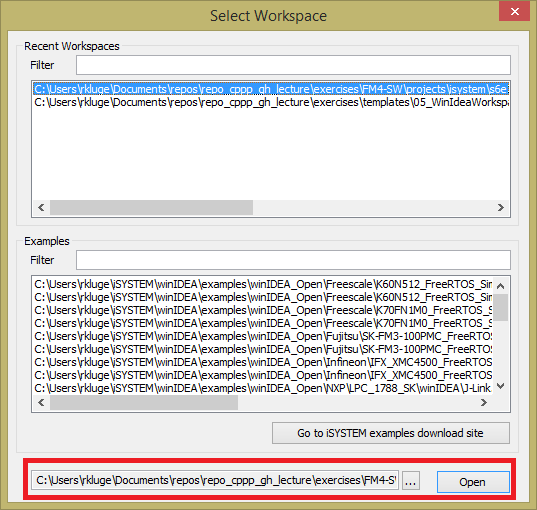
\includegraphics[width=.5\textwidth]{./05_c/figures/WinIDEASelectWorkspace.png}
\caption{Workspace-Auswahl in WinIDEA}
\label{fig:WinIdeaSelectWorkspace}
\end{centering}
\end{figure}

\item 
\RKi{Continue here: Überblick über IDE, Beispieprogramm öffnen, compilieren, downloaded, testen}
\end{enumerate}

\section{\ExercisePrefixEmbeddedC Taster abfragen \optional}

In dieser Aufgabe erweitern wir die vorherige Aufgabe um eine Benutzerinteraktion über den \textbf{User Button}.
Ziel dieser Aufgabe ist es, mit dem User Button die RGB-LED in zwei verschiedenen Szenarien zu kontrollieren.
Bei ersten Szenario soll es möglich sein die LED per Lichtschalter an und auszuschalten und beim zweiten Szenario soll die LED immer dann leuchten, wenn der \textbf{User Button} gedrückt ist.

\begin{enumerate}
\item 
Zunächst werden wir die nötigen Variablen in \textbf{button.h} deklarieren. Lege dir in der bekannten Weise zwei Zeiger auf die Direction und Value Register der blauen LED an. Weiterhin soll für den Lichtschalter der aktuelle Zustand der LED in einem unsigned 8 Bit Integer \textbf{LEDstatus} gespeichert werden.

\item Als User Button soll der digitale Button des Joystick 1, welcher an den Pin F5 des Mikrocontrollers angeschlossen ist, verwendet werden. Die Funktion \textbf{initLED()} soll den LED-Status, den Pin F5 und die blaue LED initialisieren. Der LED-Status soll zu Beginn 0 sein, und Pin F5 soll durch die Methode \textbf{Gpio1pin\_InitIn(pin, option) }initialiseren werden. Diese Funktion ist eine weitere Möglichkeit Pins des Mikrocontroller zu initialiseren. \textbf{Gpio1pin\_InitIn} intialisiert einen Pin als Eingang und kann zusätzlich zu diesem einen Pull-Up-Widerstand schalten, um das ankommende Signal zu verstärken. Der Name des Pins kann mit \textbf{GPIO1PIN\_PF5} angegeben werden und Pull-Up kann mit \textbf{Gpio1pin\_InitPullup(1u)} aktiviert werden. Abschließend soll die blaue LED in der dir bekannten Weise initialisiert werden. 

\item Mit \textbf{toggleBlueLED()} soll es möglich sein den Status der LED zu verändern. Demnach soll bei jedem Aufruf von \textbf{toggleBlueLED} der aktuelle Wert des Status invertiert werden. Der aktuelle Status der LED kann mit \textbf{setBlueLED(uint8\_t status)} gesetzt werden. 

\item Mithilfe der zuvor implementierten Funktionen sollen nun \textbf{ButtonToggleBlueLED()} und \textbf{ButtonHoldBlueLEDOn()} implementiert werden. \textbf{ButtonToggleBlueLED()} soll dem Button die Funktion eines Lichtschalters geben und  \textbf{ButtonHoldBlueLEDOn()} soll die LED zum leuchten bringen, solange der Button gedrückt gehalten wird. 

\end{enumerate}
\hints{
	\item Mit dem Aufruf \textbf{Gpio1pin\_Get(GPIO1PIN\_PF5)} kann der aktuelle Wert des Pin F5 ausgelesen werden.
	
	\item Es ist zu beachten, dass durch einen Pull-Up-Widerstand, sich die Spannung am Mikrocontroller invertiert. Folglich ist bei gedrückten Joystick das Eingangssignal am Mikrocontroller 0 und bei losgelassenem Button 1. 
	
	\item \textbf{while(Gpio1pin\_Get(GPIO1PIN\_PF5) == 0)} kann verwendet werden, um das Programm solange zu pausieren bis der Button losgelassen wird. 
}

\section{\ExercisePrefixEmbeddedC Touchdisplay ansteuern \optional}

\RKi{Ziel: (i) Regelmäßiges Muster ausgeben (Schachbrett, Blockschachbrett,...); (ii) Text ausgeben (s. writeText(char[]))}

\section{\ExercisePrefixEmbeddedC Joysticks abfragen \optional}

\RKi{Ziel: (i) Joystick-Daten auslesen und (ii) auf dem Display ausgeben. Die Studenten können entweder ihr eigene writeText-Funktion nutzen oder auf die Musterlösung der vorirgen Aufgabe zugreifen.}
\section{\ExercisePrefixEmbeddedC Touchscreen ansteuern \optional}
Eingebaut im mit dem Mikrocontroller verbundenen Bildschirm ist eine resistive 4-Wire Touchschicht.
Der Name setzt sich zusammen aus den Eigenschaften dieser Schaltung.
Resistiv steht für die Messung von Widerständen zum Erkennen von Touch-Gesten und 4-Wire, da für diese Durchführung vier Datenleitungen gebraucht werden.
Ein resistiver 4-Wire-Touchscreen ist wie in \Cref{fig:rsTouch} aufgebaut.
%
\begin{figure}[htbp]
    \centering
    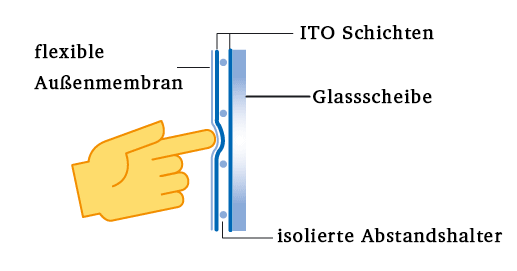
\includegraphics[width=0.35\textwidth]{./05_c/figures/4WireRSTouch.png}
    \caption{Aufbau eines resistiven Touchscreens}
    \label{fig:rsTouch}
\end{figure}
%
Dieser besteht aus
\begin{inparaenum}
\item
einer Glas- oder Acryl-Schicht,
\item 
einer äußeren resistiven Schicht die mit Indium-Zinn-Oxid (\enquote{indium tin oxide}, ITO) beschichtet ist,
\item 
isolierenden Punkten,
\item 
der inneren resistiven Schicht aus ITO und 
\item
einem Polyester-Film.
\end{inparaenum}
Die beiden resistiven Schichten sind jeweils an 2 Polen angeschlossen (\Cref{fig:fourRSTouch}).
%
\begin{figure}[htbp]
    \centering
    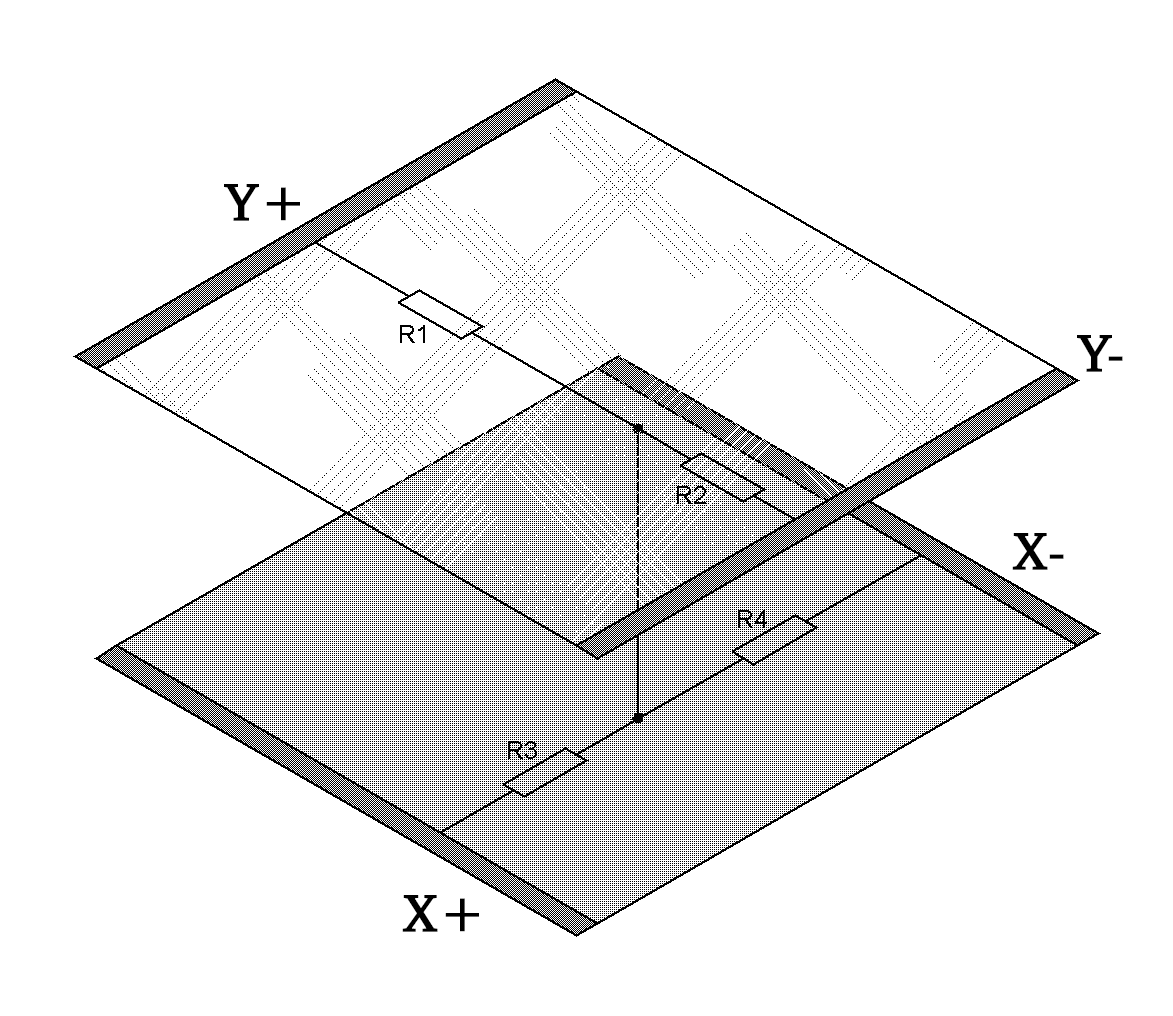
\includegraphics[width=0.3\textwidth]{./05_c/figures/ResistiveTS.png}
    \caption{Aufbau eines 4-Wire resistiven Touchscreens }
    \label{fig:fourRSTouch}
\end{figure} 
%
Die Schichten sind in Bezug auf ihre Pole um 90 Grad zueinander gedreht.
Dies ist wichtig, um später die X- und Y-Koordinaten des Druckpunkts zu lesen.
Sobald ein Objekt die oberste Glas- oder Acryl-Schicht berührt und genügend Druck ausübt, wird sich die oberste ITO-Schicht mit der unteren verbinden.
Die X- und Y-Koordinate des Druckpunkts wird bestimmt, indem die Spannungen an den Polen gemessen werden.
Zur Messung des X-Wertes werden X+ und X- über Gleichspannung geschaltet.
Das heißt, X+ ist beispielsweise auf Vcc und X- ist mit GND verbunden.
Durch die Verbindung der beiden ITO-Schichten entsteht ein Stromfluss durch beide Schichten und es kommt zu einem Spannungsteiler in der X-Schicht.
Die Spannungen zwischen X+ und dem Druckpunkt sowie dem Druckpunkt und X- lassen sich durch das Ausmessen von Y- und Y+ auslesen.
Diese Information wird vom Microcontroller ausgelesen, der die gemessene Spannung in Relation zur Auflösung des Displays setzt.
Die Y-Koordinate wird gemessen, indem Y+ und Y- an eine Gleichspannung gelegt und die Spannungen an X+ und X- ausgelesen werden.

Für dein Projekt stellen wir dir die Funktionen \lstinline|readTouchX()|, \lstinline|readTouchY()| und \lstinline|readTouchZ()| zur Verfügung, die X-, Y- und Z-Werte eines Druckpunkts auf dem Touchscreen auslesen können (\filename{analog.h}).
Ist der Z-Wert größer als ein bestimmter Grenzwert, kann von einer Berührung des Touchscreens ausgegangen werden. 


\subsection{Werte des Touchscreens debuggen}
Implementiere zunächst die Funktion \lstinline|debugTouch()|, die kontinuierlich die X-,Y- und Z-Werte des Touchscreens auf dem Bildschirm ausgibt.

\subsection{Zeichnen auf dem Touchscreen}
In diesem Abschnitt implementierst du eine kleine Mal-Anwendung für den Touchscreen.
Mit dieser soll es möglich sein, verschiedene Farben auszuwählen und mithilfe des Fingers auf dem Bildschirm zu zeichnen.
Vervollständige hierfür die Funktion \lstinline|paintTouch()|.
Bereits implementiert sind die Farbpaletten und der Lösch-Button auf der unteren Seite des Bildschirms.
Die Funktion \lstinline|printTouch()| muss noch um eine Touch-Logik ergänzt werden, die Berührungspunkte auf dem Bildschirm erkennt und diese korrekt interpretiert.
Hierbei gibt es folgende Szenarien:
\begin{itemize}
\item 
Die Farbpalette wird berührt und somit verändert sich die aktuelle Malfarbe.
\item 
Bild erneuern wurde gedrückt und der Malbereich wird zurückgesetzt.
\item 
Wird der freie Zeichen-Bereich berührt, so soll an dieser Stelle in der ausgewählten Farbe ein ausgefüllter Kreis mit dem Radius \lstinline|PENRADIUS| gezeichnet werden.
\end{itemize}
\Cref{fig:paintTouch} zeigt, wie die Anwendung fertig aussehen kann.
\begin{figure}[htbp]
	\centering
	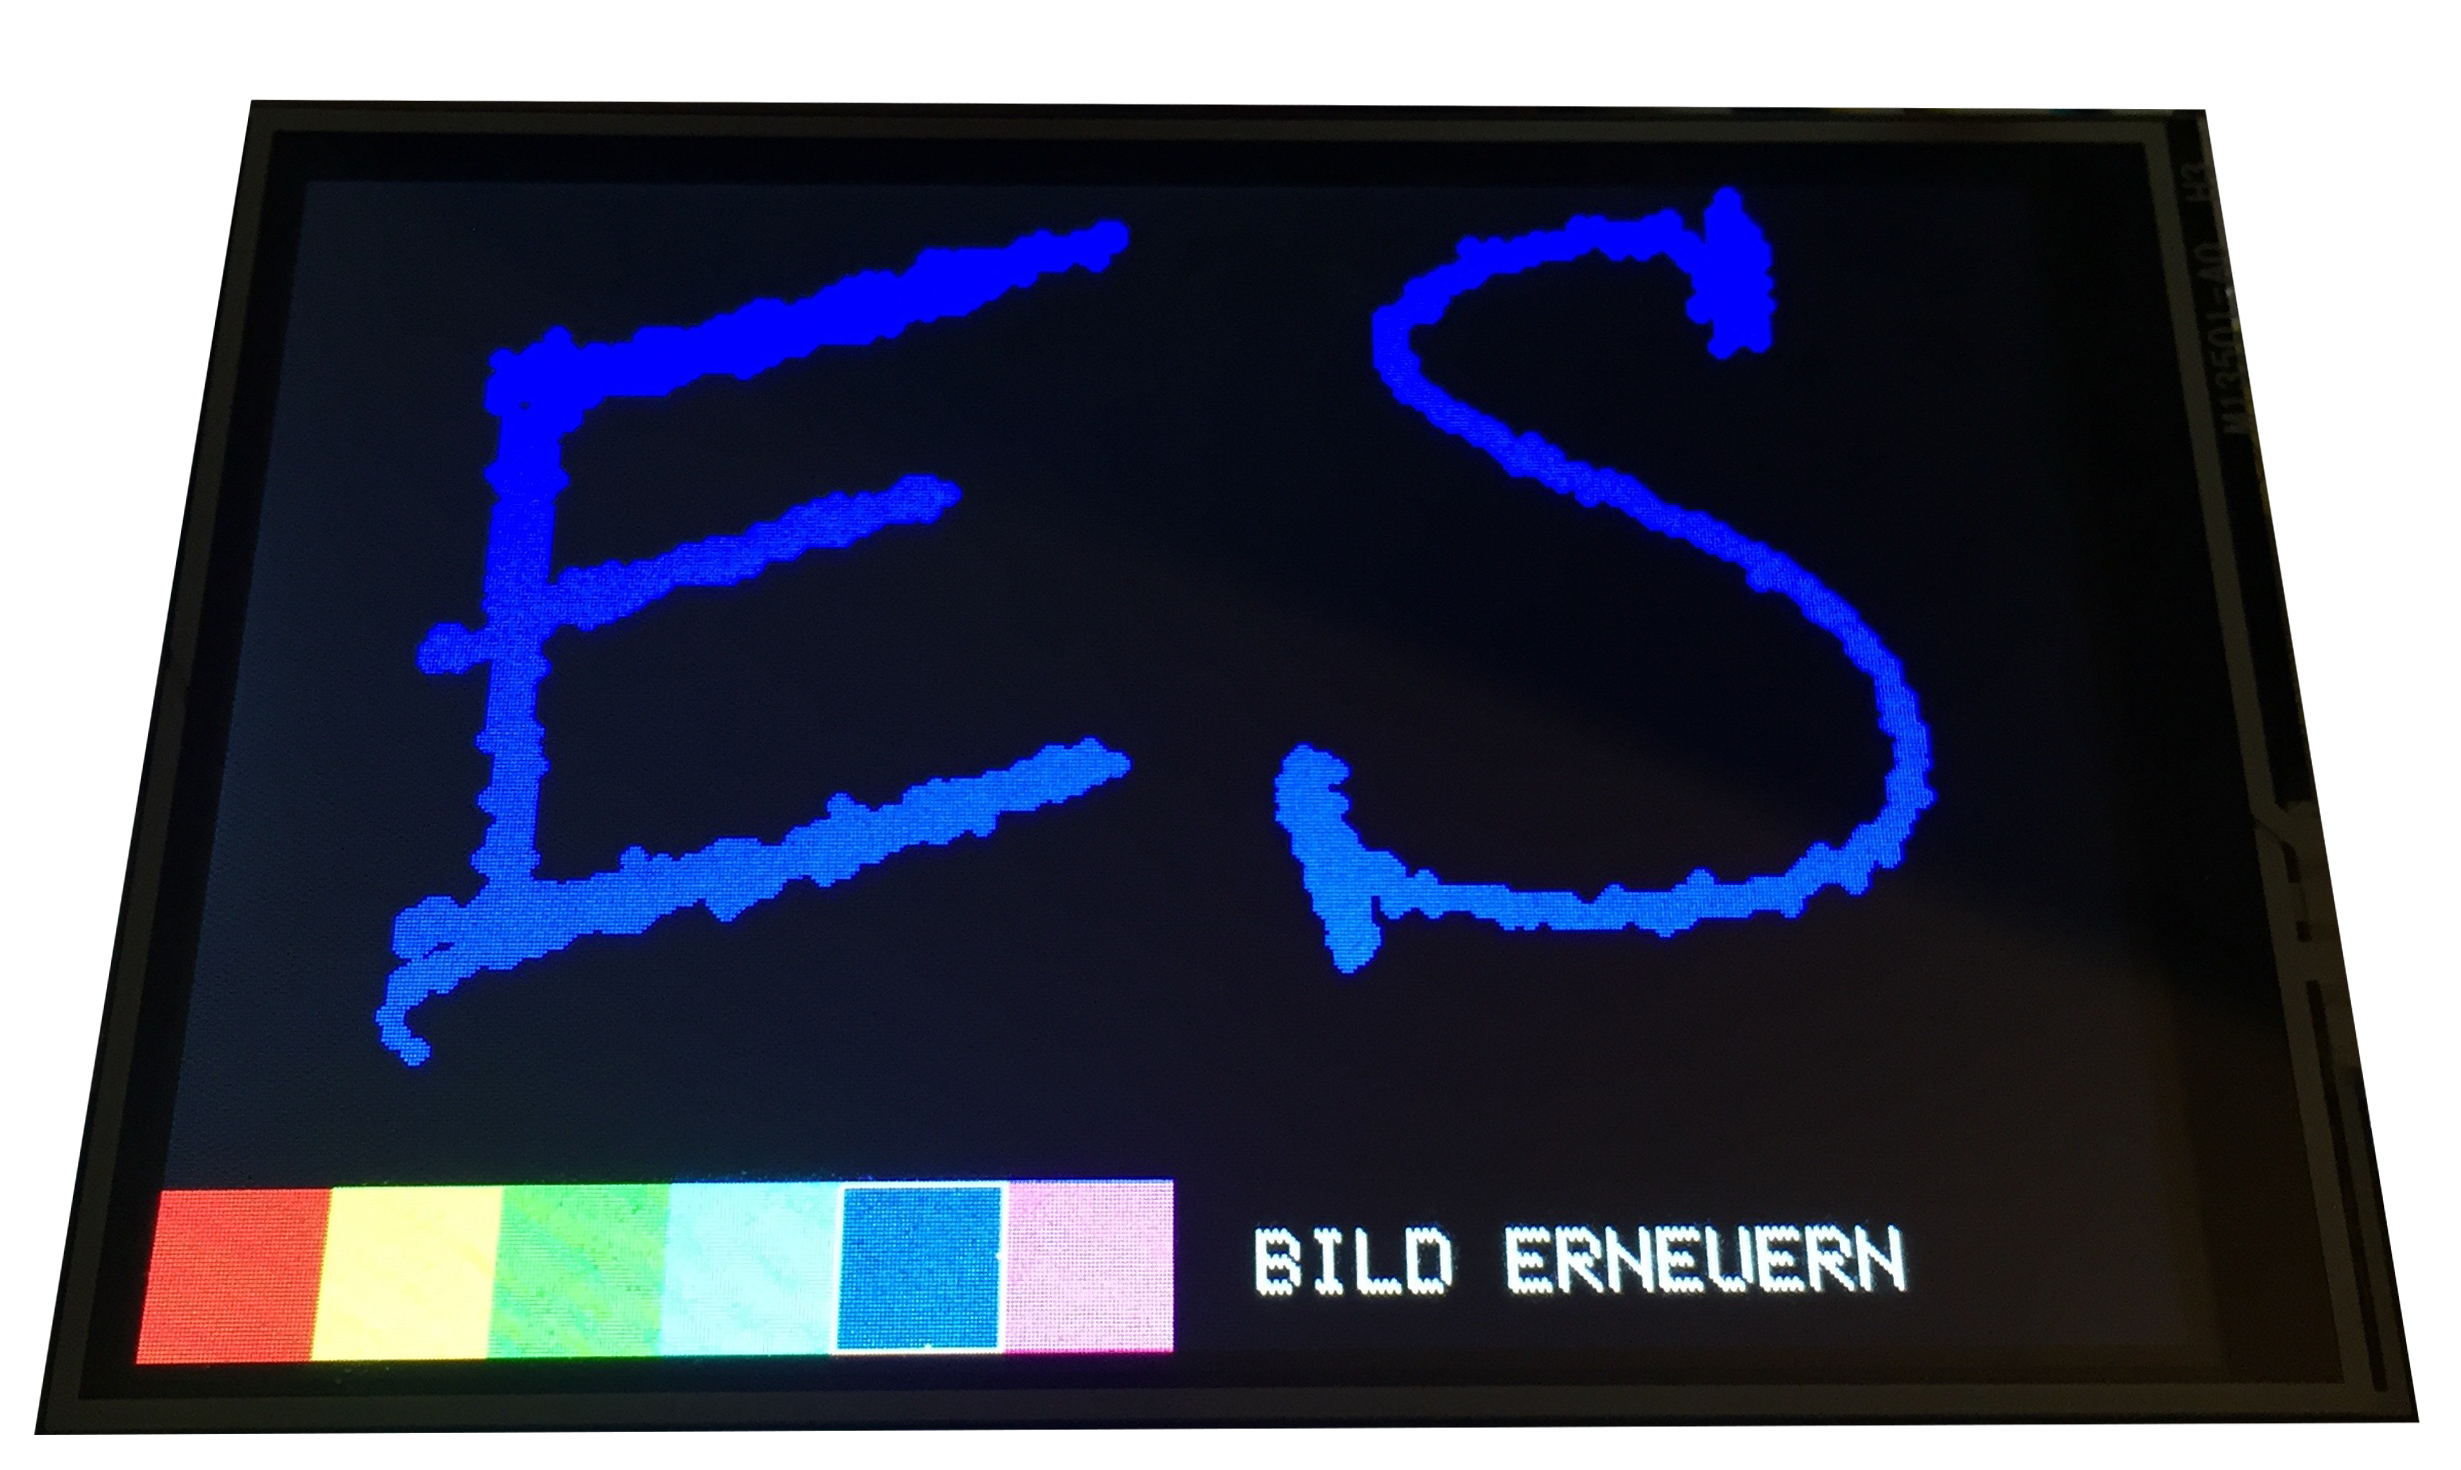
\includegraphics[width=0.3\textwidth]{./05_c/figures/Paint-Szenario.png}
	\caption{Mal-Anwendung auf dem Touchscreen}
	\label{fig:paintTouch}
\end{figure} 
\section{\ExercisePrefixEmbeddedC Eigenes Microcontroller-Projekt umsetzen \optional}

Nachdem du einige der Ein- und Ausgabemöglichkeiten des Boards kennengelernt hast, besteht deine Aufgabe in diesem Teil darin, ein kleines Projekt deiner Wahl umzusetzen.
Du hast hierbei die freie Wahl, die folgenden Vorschläge sollen nur als Anregung dienen.

\subsection*{Vorschlag: Pong}
Zwei Gegner sollen je einen Balken (Rechteck) am linken oder rechten Rand des Spielfeldes mit den Schiebereglern steuern können, um einen Ball (ein Quadrat) im Spiel zu halten.
Erreicht der Ball den linken oder rechten Rand des Spielfelds, so bekommt der Spieler auf der anderen Seite einen Punkt und der Ball wird an seine Anfangsposition (die Mitte des Spielfelds) zurückversetzt.
Erreicht der Ball den oberen oder unteren Rand sowie einen der Balken der Spieler, so wird der Ball reflektiert - verlässt also niemals das Spielfeld.

Gewonnen hat der Spieler, der zuerst eine definierte Anzahl an Punkten erreicht.
Die aktuelle Punktzahl beider Spieler könnte auf der Siebensegmentanzeige ausgegeben werden.
\begin{center}
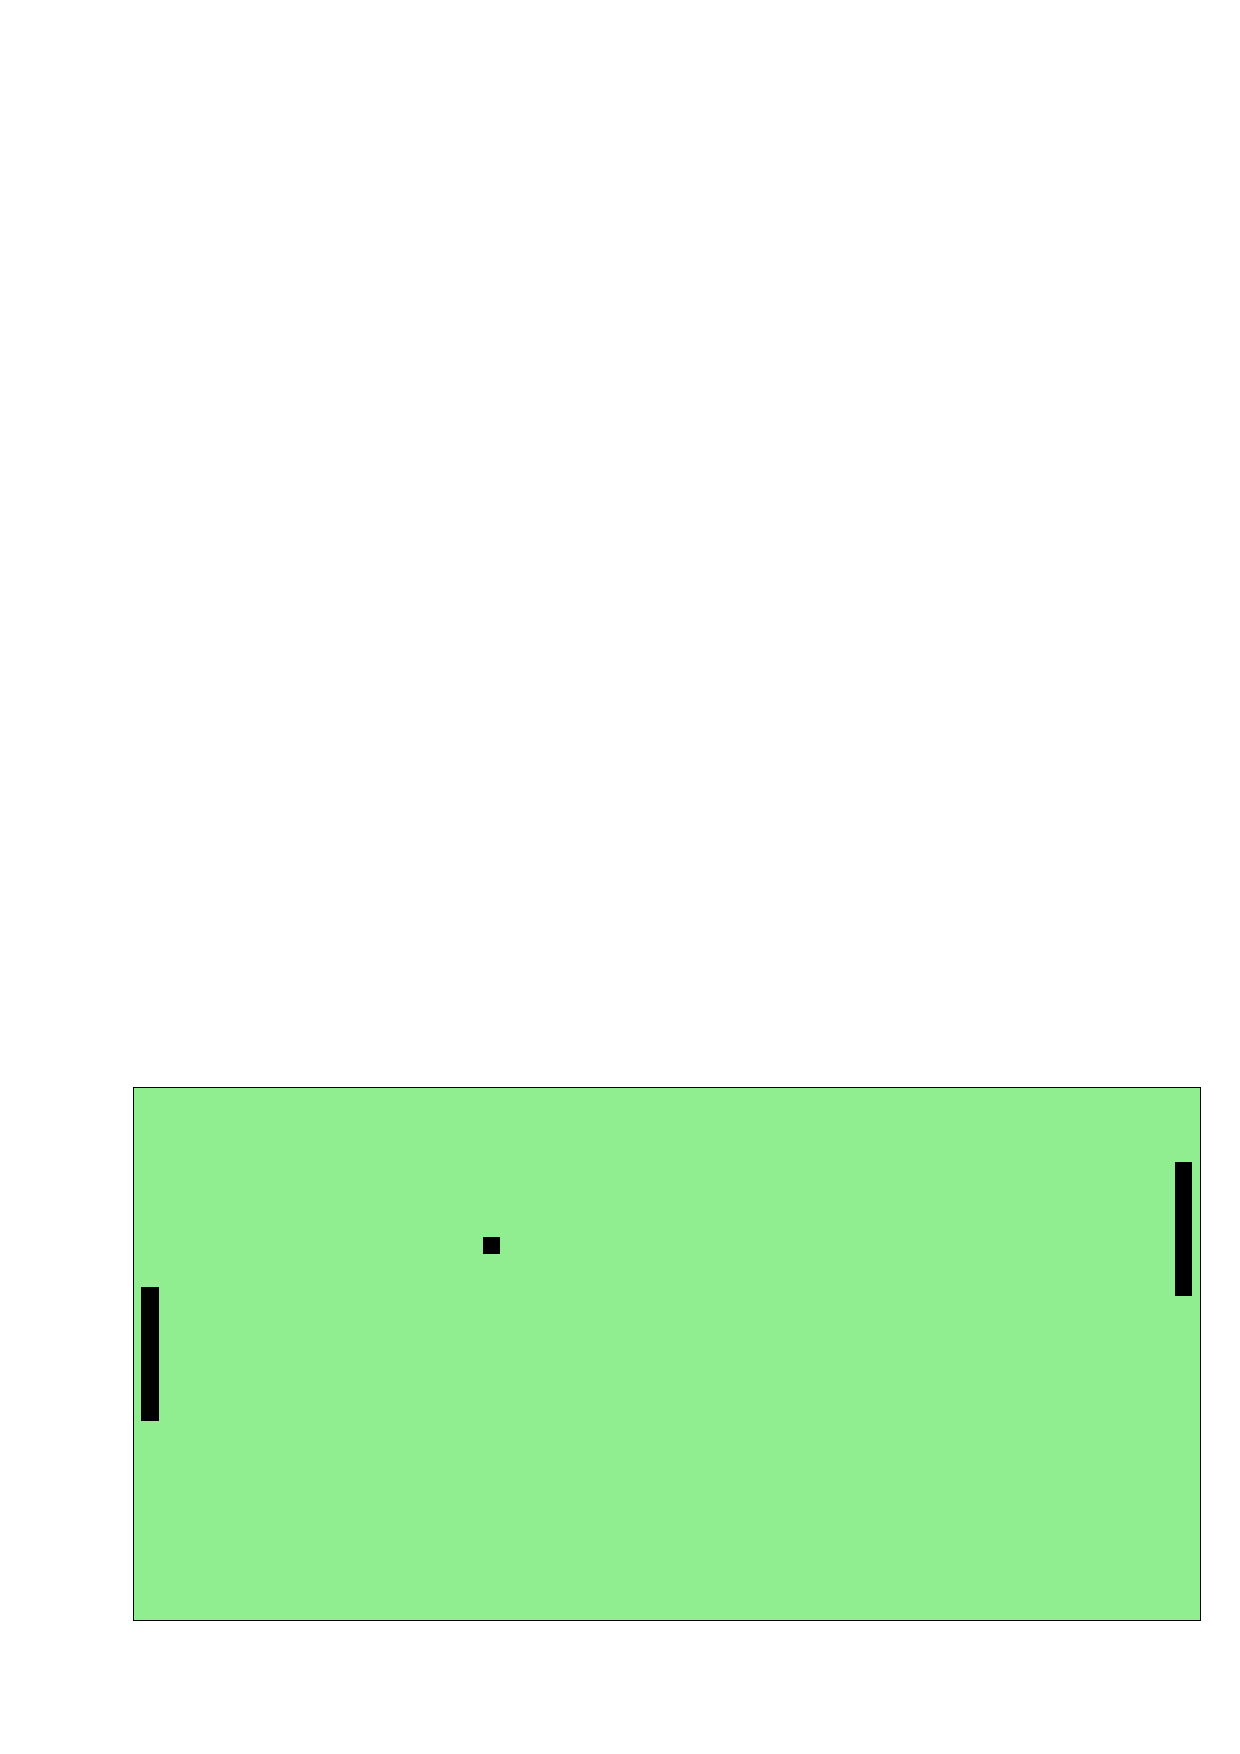
\includegraphics[scale=0.4]{05_c/figures/pong}
\end{center}



\subsection*{Vorschlag: Game of Life}
\glqq{}Game of Life\grqq{}\footnote{siehe auch \url{http://de.wikipedia.org/wiki/Conways_Spiel_des_Lebens}} besteht aus einem zweidimensionalen Spielfeld.
Jedes Feld steht für eine Zelle, die \textit{tot} (grün) oder \textit{lebendig} (schwarz) ist.
Jede Zelle hat acht Nachbarzellen, die ebenso tot oder lebendig sein können.
Zu Beginn gibt es eine vordefinierte Anfangsgeneration.
%
Durch festgelegte Regeln wird die nachfolgende Generation ermittelt:
\begin{itemize}
	\item Eine \textbf{lebende Zelle} \dots
	\begin{itemize}
		\item mit 1 oder 0 lebenden Nachbarn stirbt aus Einsamkeit.
		\item mit 4 oder mehr lebenden Nachbarn stirbt wegen Übervölkerung.
		\item mit 2 oder 3 lebenden Nachbarn bleibt am Leben.
	\end{itemize}
	\item Eine \textbf{tote Zelle} mit genau 3 lebenden Nachbarn wird in der nächsten Generation geboren werden, andernfalls bleibt sie tot.
\end{itemize}
%
Als Anfangsgeneration eignen sich zufällige Populationen oder eine der folgenden Figuren:
\begin{center}
	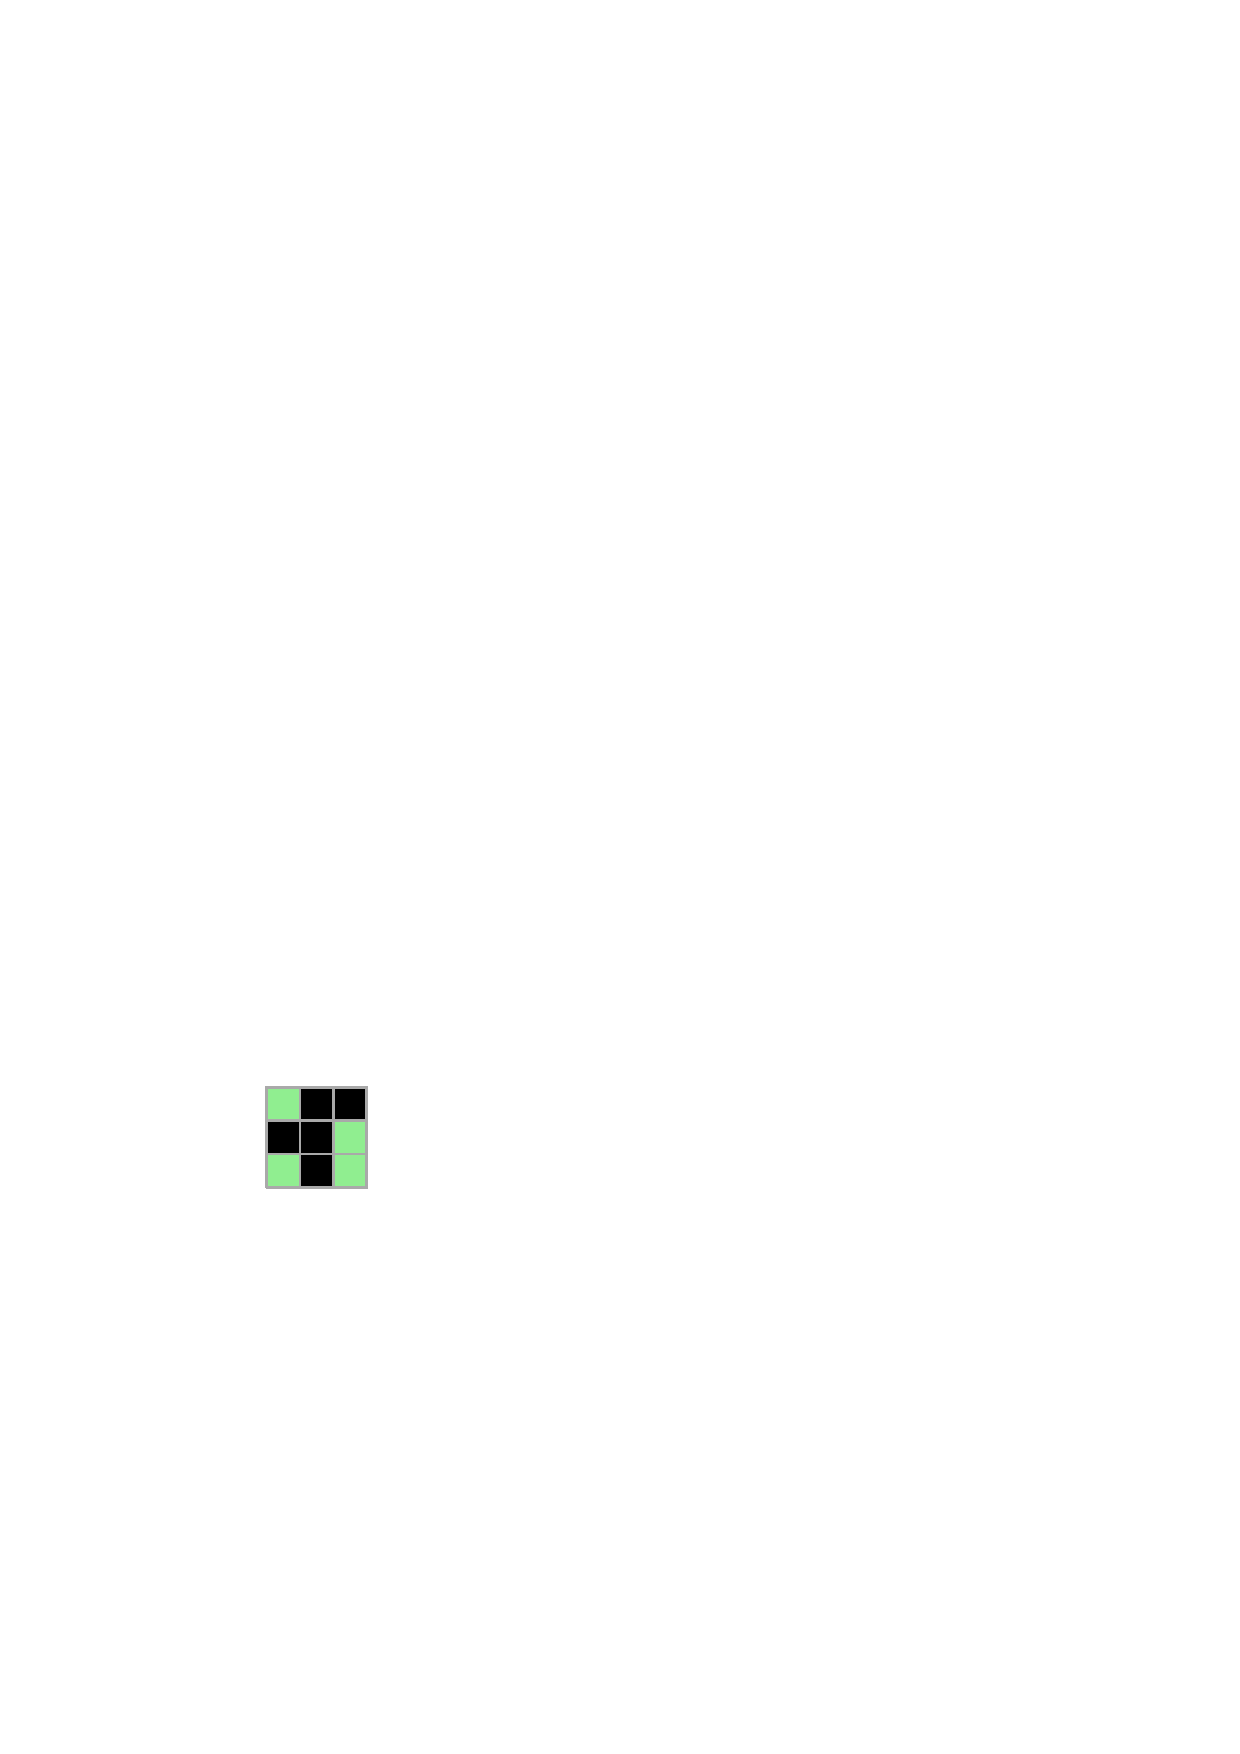
\includegraphics[scale=1]{05_c/figures/gol_init1}
	\hspace{5mm}
	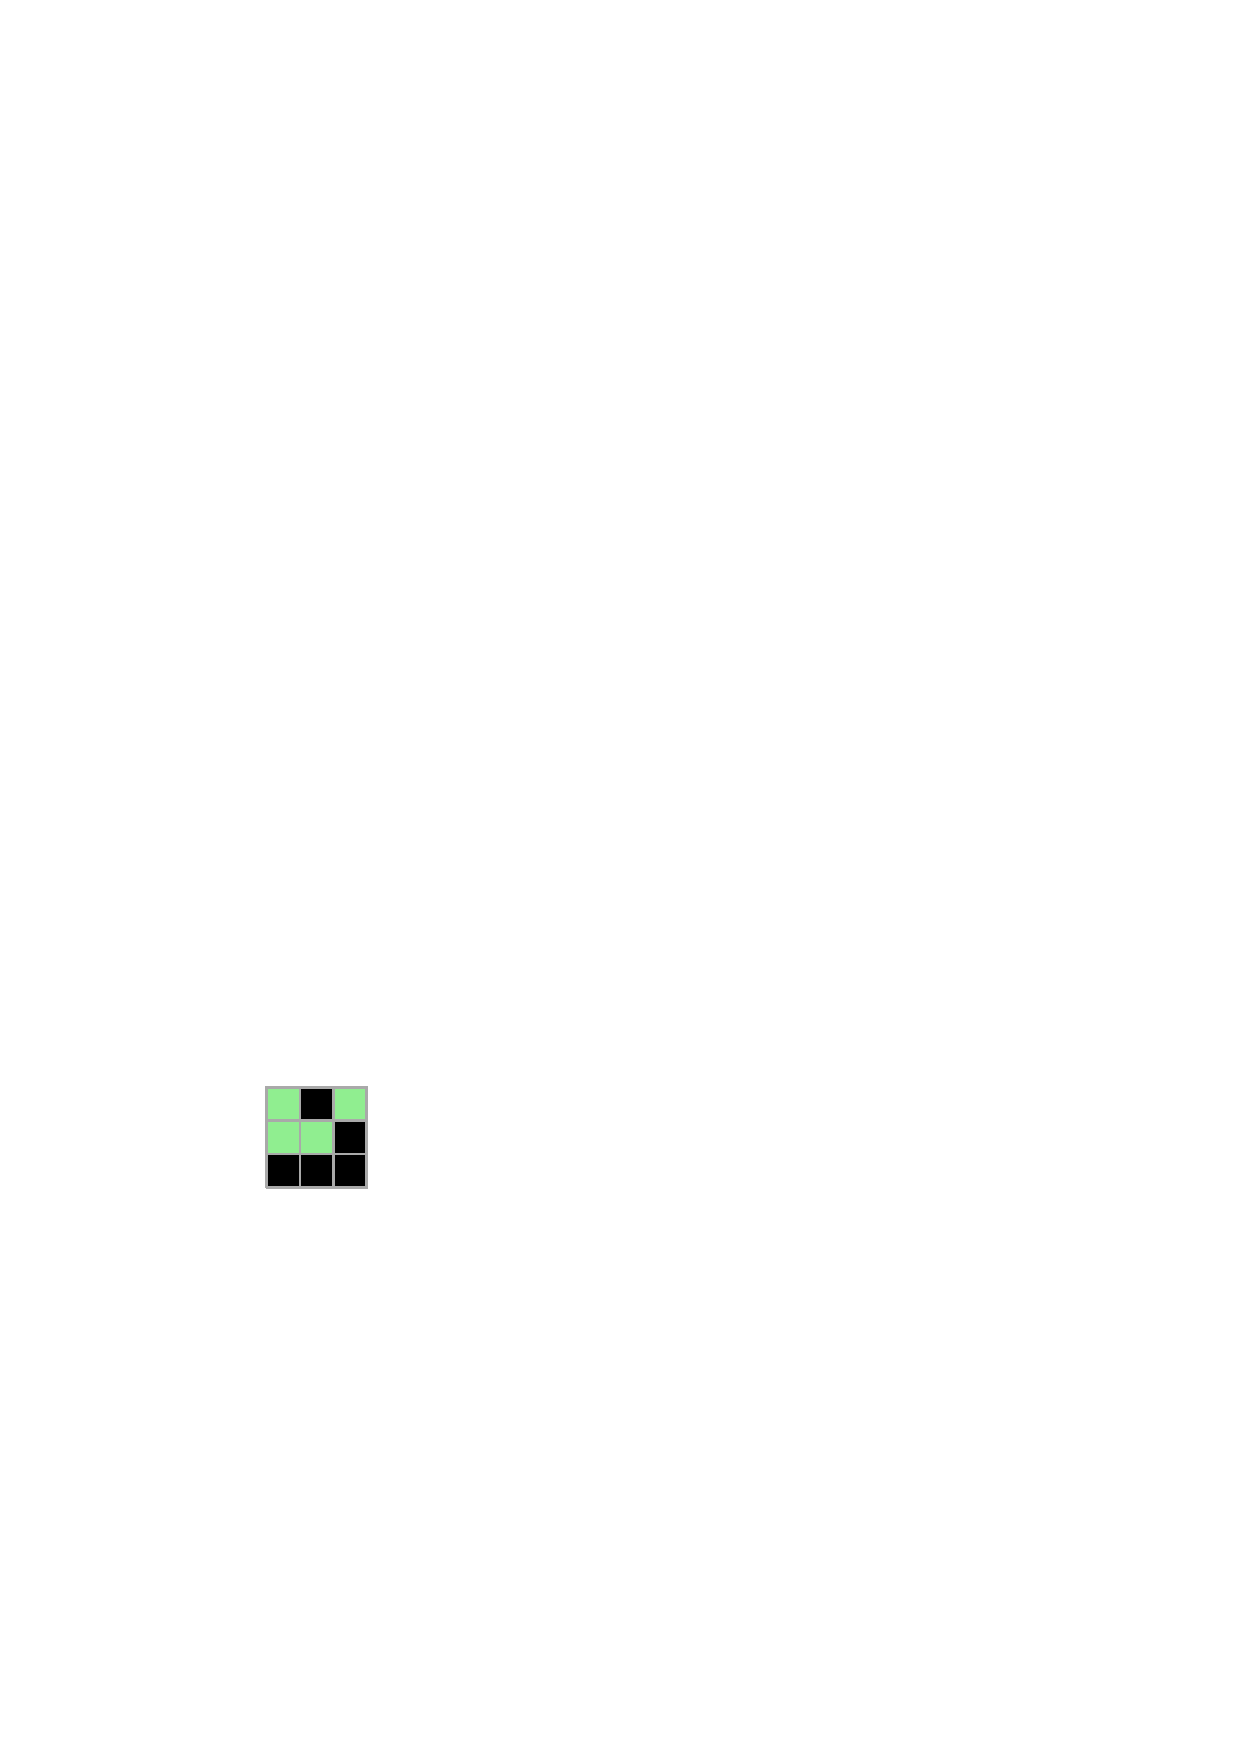
\includegraphics[scale=1]{05_c/figures/gol_init2}
	\hspace{5mm}
	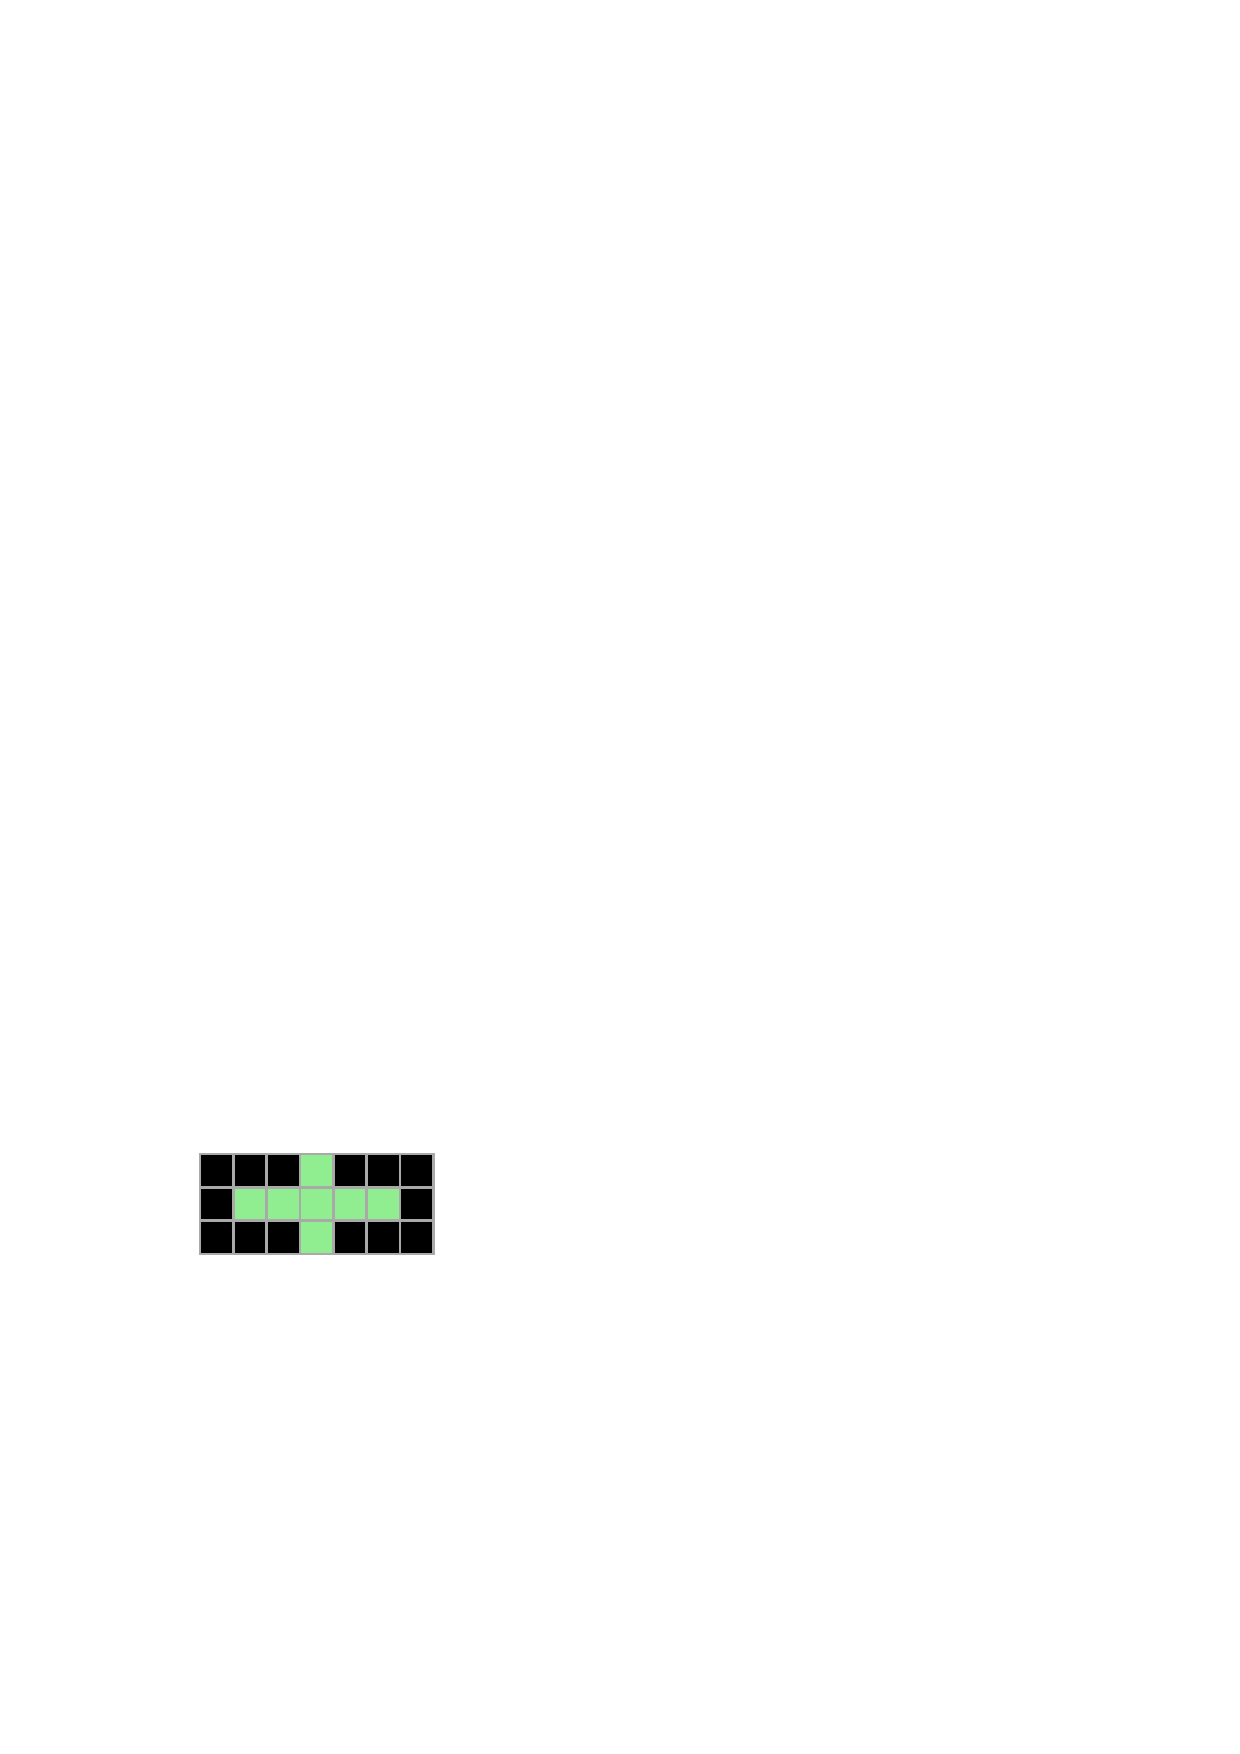
\includegraphics[scale=1]{05_c/figures/gol_init3}
\end{center}
%
\hints{
	\item Da das Spielfeld begrenzt ist, soll es torusförmig aufgebaut werden.
    Das heißt: Alles, was am unteren Rand des Spielfelds verschwindet, kommt oben wieder heraus -- das Gleiche gilt für den linken und rechten Rand. 
	\item Verwende als Spielfeld ein mehrdimensionales Array
	\item Ein weiteres mehrdimensionales Array bietet sich an, um die zukünftige Generation erzeugen zu können.
	\item Achte beim torusförmigen Feld unbedingt darauf, dass du nicht über die Grenzen des Spielfelds hinaus zugreifst!
    Das kann zu unvorhersehbarem und schwer zu debuggenen Verhalten des ganzen Displays führen!
}

\subsection*{Vorschlag: Regentropfen}

Das Touch-Display ist ein kleiner Teich;
wenn du eine Stelle mit dem Finger berührst, breitet sich von dort eine konzentrische Welle aus.
Die Geschwindigkeit der Welle kannst du zusätzlich abhängig machen vom ausgeübten Druck.


\subsection*{Weitere Vorschläge}
\RKi{Beispielbilder finden, CC4.0-kompatibel sind}
\begin{minipage}{.45\textwidth}
    \begin{center}Asteroids\\\vspace{4ex}
        %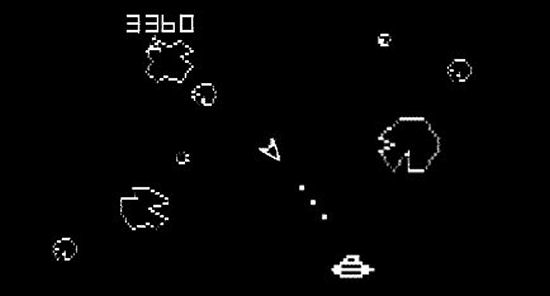
\includegraphics[width=.5\textwidth]{05_c/figures/img_asteroids.png}
    \end{center}
    \begin{center}Pacman\\\vspace{4ex}
        %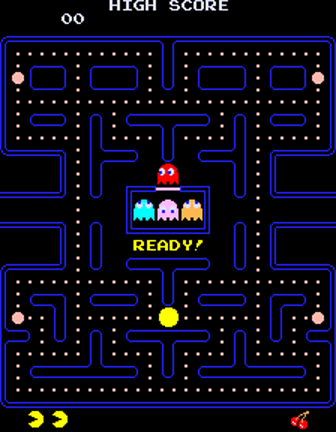
\includegraphics[width=.3\textwidth]{05_c/figures/img_pacman.png}
    \end{center}
    \begin{center}Labyrinth\\\vspace{4ex}
        %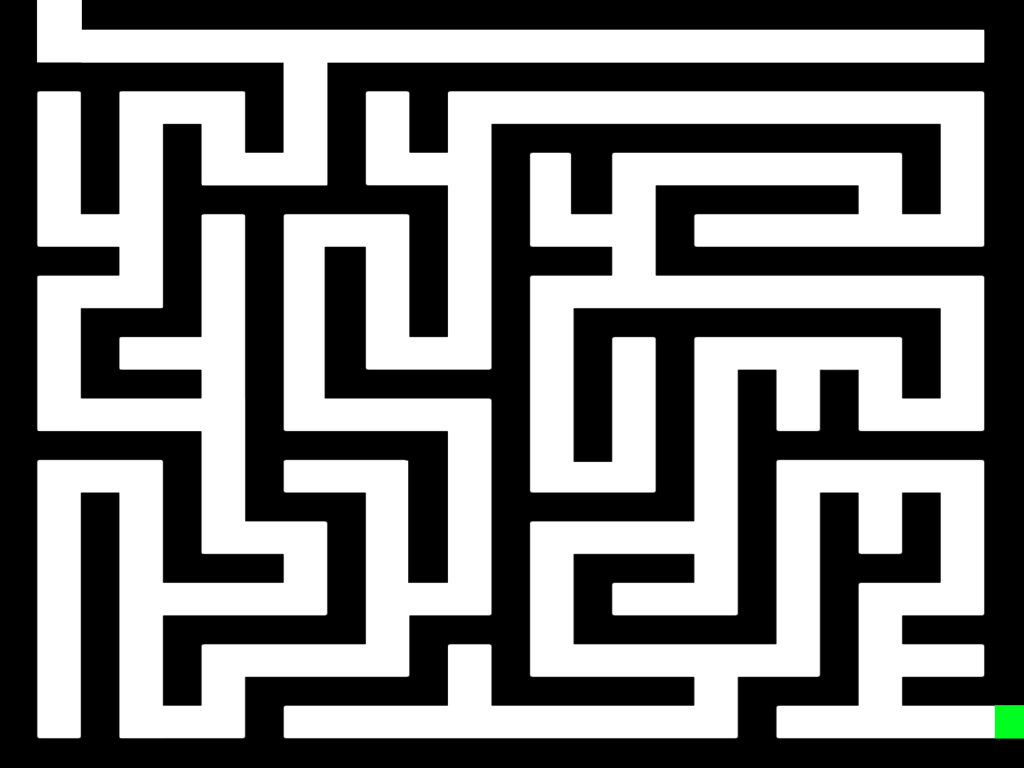
\includegraphics[width=.4\textwidth]{05_c/figures/img_maze.png}%
    \end{center}
\end{minipage}
\begin{minipage}{.45\textwidth}
	\begin{center}Ausweichspiele à la Hugo\\\vspace{4ex}
        %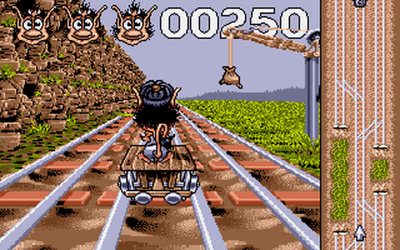
\includegraphics[width=.4\textwidth]{05_c/figures/img_hugo.png}
    \end{center}
	\begin{center}Moorhuhn\\\vspace{4ex}
        %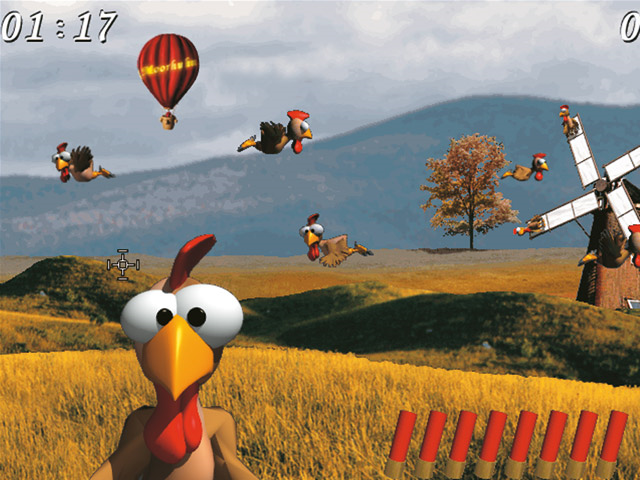
\includegraphics[width=.4\textwidth]{05_c/figures/img_moorhuhn.png}
    \end{center}
	\begin{center}Snake\\\vspace{4ex}%
       % 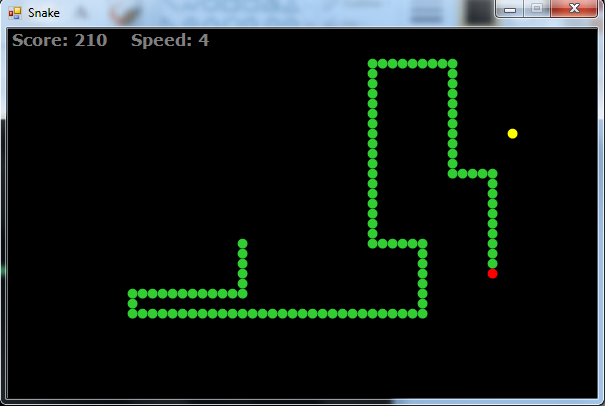
\includegraphics[width=.4\textwidth]{05_c/figures/img_snake.png}
    \end{center}
\end{minipage}


\hints{
	\item Möchte man ein Bild auf dem Board anzeigen, so empfiehlt es sich die einzelnen Pixeldaten in einem Array zu speichern.
	GIMP bietet hierfür die Möglichkeit eine Bilddatei als Header im \texttt{GIMP header image file format} zu exportieren.
	Da das Board nur zwei Farbwerte ermöglicht, sollte das Bild vor dem Exportieren über den Menüpunkt \textbf{Bild --> Modus} auf \textbf{indiziert \ldots} (Schwarz/Weiß-Palette (1-Bit)) gestellt werden.
	Anschließend kann man das \lstinline{header_data} Array verwenden, um auf die Bilddaten zuzugreifen.
}


\newpage
\setHeader{Zusatzaufgaben}
\section{Eigene Arrays (optional)}
\label{sec:array}

Nachdem du bei unseren Übungen zu Arrays gesehen hast, dass es störend ist, wenn man die Größe eines Arrays immer getrennt zu den gespeicherten Daten verwalten muss, ist ein sinnvoller Schritt, eine eigene Array-Klasse zu implementieren, die Daten und Größe des Arrays zusammen speichert.

Eine möglicher Anwendungsfall sieht so aus:

\begin{lstlisting}
#include "Array.h"
#include <iostream>
#include <string>

template<typename T>
void printFirst(const Array<T> &array) {
    std::cout << array[0] << std::endl;
}

int main() {
    Array<std::string> stringArray(10);
    stringArray[0] = "Hello World";
    printFirst(stringArray);
}
\end{lstlisting}

\emph{Hinweise}:
\begin{itemize}
\item
Überlege dir, welche Operatoren/Methoden das obige Code-Beispiel von Array verlangt.
Unter anderem musst du jeweils einen \lstinline{const} und einen nicht-\lstinline{const} \lstinline{operator[]} implementieren.

\item
Du kannst auch Exceptions (z.B. \lstinline{std::out\_of\_range} aus \lstinline{<stdexcept>}) verwenden, um falsche Indices korrekt abzufangen.

\item
Eine fortgeschrittene Übung ist es, Iteratoren oder \lstinline{operator+(unsigned int)} für \lstinline|Array| bereitszustellen, sodass du z.B. die Funktion \lstinline{std::copy} aus der Standardbibliothek verwenden kannst, um ein Array zu kopieren:
\begin{lstlisting}
#include <algorithm> // copy
#include <iterator> // back_inserter
#include <vector>
// ...
Array<int> array(10);
std::vector<int> vector;
std::copy(array, array + 4, std::back_inserter(vector));
\end{lstlisting}

\item
\LKi{Eclipse-spezifisch}
Diese Idee ist natürlich nicht neu.
Seit C++11 gibt es eine Array-Implementation in der C++-Standardbibliothek (\lstinline{std::array}\footnote{\url{http://www.boost.org/doc/libs/1_55_0/doc/html/array.html}}).
Du findest die gleiche Klasse auch als \lstinline{boost::array} in Boost.
Wenn du damit experimentieren willst, mussst du die Compiler-Unterstützung für C++11 einschalten.
Gehe dazu in die Projekteigenschaften (\emph{Rechtsklick} $\to$ Properties) und setzte unter \emph{C/C++-Build/Settings/GCC C++ Compiler/Dialect} das Feld \emph{Language Standard} auf \emph{ISO C++11}.
\end{itemize}

\newpage
\section{Callbacks}

\paragraph*{Motivation für Callbacks}
In dieser Aufgabe werden mehrere Methoden zur Realisierung von Callbacks in C++ vorgestellt und implementiert.
Callbacks können als Alternative zum Observer Pattern\footnote{\url{http://de.wikipedia.org/wiki/Observer_Pattern}} eingesetzt werden.
Beispielsweise kann man einem GUI-Button eine Callback-Funktion übergeben, die aufgerufen werden soll, sobald der Button gedrückt wird.
Wir werden Callbacks dazu verwenden, um den Benutzer bei jedem Schritt eines laufenden Algorithmus über den aktuellen Fortschritt zu informieren.

\subsection{Basisalgorithmus}
Implementiere folgenden Algorithmus, der das Problem der Türme von Hanoi löst.\footnote{\url{http://de.wikipedia.org/wiki/Turm_von_Hanoi}}\\
\begin{algorithm}[H]
 \SetAlgoLined
 \textbf{funktion} hanoi (\textbf{Number} i, \textbf{Pile} a, \textbf{Pile} b, \textbf{Pile} c) { \\
     \If{i > 0} {
        hanoi(i-1, a, c, b); \tcp{Move i-1 slices from pile ''a'' to ''b''}
        Move slice from ''a'' to ''c''; \\
        hanoi(i-1, b, a, c); \tcp{Move i-1 slices from pile ''b'' to ''c''}
     }
 }
\end{algorithm}

Du brauchst keine Türme zu modellieren und zu verschieben, es reicht, lediglich eine Ausgabe auf die Konsole zu machen. Bei einem Aufruf von \textbf{hanoi(3, 1, 2, 3)} soll folgende Ausgabe erfolgen:
\begin{lstlisting}
1 -> 3
1 -> 2
3 -> 2
1 -> 3
2 -> 1
2 -> 3
1 -> 3
\end{lstlisting}

\subsection{Callbacks mit Funktionszeigern}
Nun wollen wir die fest einprogrammierte Ausgabe durch ein Callback ersetzen. Dadurch wird es möglich, die Funktion auszutauschen und z.B. eine graphische Ausgabe zu implementieren, ohne jedoch den Algorithmus selbst zu ändern.

Eine simple Art des Callbacks, die auch in C verfügbar ist, ist die Übergabe eines Funktionszeigers, der die Adresse der aufzurufenden Funktion beinhaltet.
Ändere deine Implementation entsprechend um:

\begin{lstlisting}
void hanoi(int i, int a, int b, int c, void(*callback)(int from, int to)) {
	...
	callback(a, c);
	...
}
\end{lstlisting}

Nun können wir eine Funktion mit zwei Parametern an \lstinline{hanoi()} übergeben.
\begin{lstlisting}
void print(int from, int to) {
	cout << from << " -> " << to << endl;
}
...
hanoi(3, 1, 2, 3, print);
\end{lstlisting}

\subsection{Callbacks mit Funktoren}
Ein Nachteil der vorherigen Implementation ist, dass nur reine Funktionen als Callback übergeben werden können.
Eine Möglichkeit dies zu umgehen ist die Verwendung von Templates.
Der Callback-Typ wird dabei durch einen Template-Parameter spezifiziert:
\begin{lstlisting}
template<typename T>
void hanoi(int i, int a, int b, int c, T callback) ...
\end{lstlisting}

Dadurch kann an \lstinline{hanoi()} fast alles übergeben werden, was sich syntaktisch mittels
\begin{lstlisting}
	callback(a, c);
\end{lstlisting}
aufrufen lässt, also auch Objekte, bei denen der $()$ Operator überladen ist (sog. \emph{Funktoren}\footnote{\url{https://de.wikipedia.org/wiki/Funktionsobjekt}}).
Dabei müssen nicht einmal die Parametertypen (\lstinline{int}) exakt übereinstimmen, solange eine implizite Umwandlung durch den Compiler möglich ist.

Teste deine Implementation mit einem Funktor.
Schreibe dafür eine einfache Klasse und überlade deren \lstinline{operator()}:
\begin{lstlisting}
	void operator()(int from, int to);
\end{lstlisting}

\subsection{Callbacks mit \lstinline{Callback}-Klasse}

\paragraph*{Probleme der bisherigen Implementation}
Die Verwendung von Templates hat uns zwar eine sehr flexible und syntaktisch ansprechende Möglichkeit für Callbacks geliefert, beherbergt jedoch mehrere, teils gravierende, Schattenseiten.

Zum einen ist es dadurch immer noch nicht möglich, beliebige Methoden einer Klasse als Callback zu übergeben.
Durch Methodencallbacks könnten Klassen mehrere unabhängige Callback-Methoden besitzen.
Zum anderen ist \lstinline{hanoi} nun an den Callback-Typ \textbf{gekoppelt}.
Wenn wir also \lstinline{hanoi} selbst an eine Funktion/Methode übergeben wollen, muss der Callback-Typ bei der Übergabe mit angegeben werden und zerstört somit die Unabhängigkeit der Funktion von ihrem Callback.
Dies kann sich insbesondere bei komplexeren Anwendungen von Callbacks sehr negativ widerspiegeln.
Stell dir vor, du hättest ein GUI-Framework mit verschiedenen Elementen, die Callbacks nutzen, z.B. Buttons.
Dann wäre die Button-Klasse ebenfalls an den Callback-Typ gekoppelt.
Immer wenn ein Button als Parameter an eine Funktion übergeben wird, müsste diese Funktion den Callbacktyp ebenfalls als Template-Parameter entgegennehmen:

\begin{lstlisting}
template<typename T>
void doSomethingWithButton(Button<T> &btn);
\end{lstlisting}

Dieser Stil würde sich durch das gesamte Framework ziehen, und sowohl den Entwicklungsaufwand als auch die Verständlichkeit beeinträchtigen.
Ein weiterer Nachteil wäre, dass der Callback-Typ bereits zur Kompilierzeit festgelegt werden müsste und es unmöglich wäre, diesen während der Laufzeit zu ändern.

\paragraph*{Lösung mittels \lstinline{Callback}-Klasse}

Deshalb werden wir eine Klasse schreiben, die beliebige Callbacks kapseln kann (\lstinline{Callback}), und nach außen hin allein von den Übergabeparametern des Callbacks abhängig ist.
Ziel ist es, folgendes zu ermöglichen:
\begin{lstlisting}
void hanoi(..., Callback callback) {
	...
	callback(a, c);
	...
}
...
hanoi(..., Callback(print)); // function callback
hanoi(..., Callback(c)); // functor callback
hanoi(..., Callback(&C::print, &c)); // method callback
\end{lstlisting}

Die Idee dahinter ist Folgendes:
Wir definieren eine abstrakte Klasse \lstinline{CallbackBase}, die eine abstrakte Methode \lstinline{void call() = 0} enthält.
Für jeden Callback-Typ (Funktionszeiger, Funktor und Methodenzeiger) wird eine Unterklasse erstellt, die \lstinline{call()} entsprechend reimplementiert.

\begin{center}
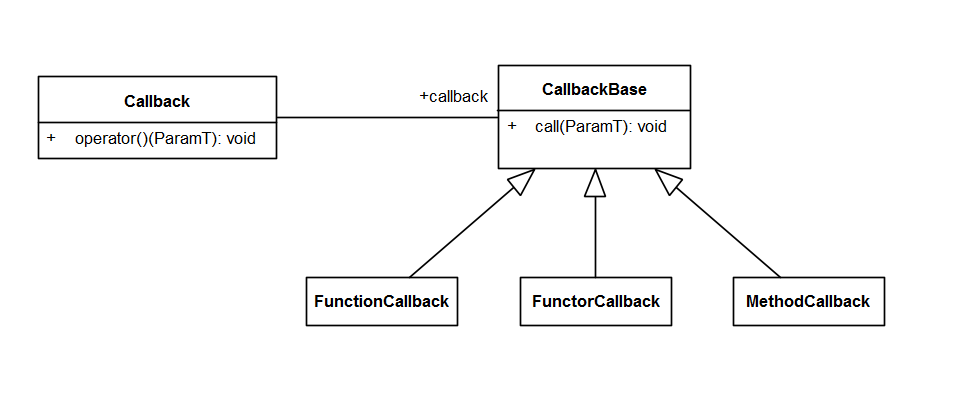
\includegraphics[width=.7\textwidth]{figures/callback_metamodel.png}
\end{center}

\paragraph*{\lstinline{CallbackBase}}

Fange mit der Klasse \lstinline{CallbackBase} an.
Damit man beim Aufrufen des Callbacks einen Parameter übergeben kann, füge \lstinline{call()} einen Parameter vom Typ \lstinline{ParamT} hinzu, wobei \lstinline{ParamT} ein Template-Parameter von \lstinline{CallbackBase} sein soll.
Der Klassenrumpf lautet also

\begin{lstlisting}
template<typename ParamT>
class CallbackBase {
public:
	...
	virtual void call(ParamT t) = 0;
};
\end{lstlisting}

Falls ein Callback eigentlich mehrere Parameter erfordert, müssen diese entsprechend in ein Containerobjekt gepackt werden.
Generische Callback-Wrapper mit variabler Parameteranzahl sind zwar möglich, würden aber den Rahmen dieses Praktikums sprengen.

\hints{
    \item Du kannst diese und alle nachfolgenden Klassen in einem einzigen Header implementieren, weil die Klassen sehr kurz sind und außerdem semantisch stark zusammenhängen.
}

\subsection{Klasse \lstinline{FunctionCallback}}
Implementiere nun die erste Unterklasse \lstinline{template<typename ParamT> FunctionCallback}, die von \lstinline{CallbackBase<ParamT>} erbt.
\lstinline{FunctionCallback} soll einen entsprechenden Funktionszeiger als Attribut besitzen, der bei der Konstruktion initialisiert wird.
Ebenso soll \lstinline{call(ParamT t)} implementiert werden, wo der gespeicherte Funktionszeiger mit dem gegebenen Argument aufgerufen wird.

Teste deine Implementation.
Lasse \lstinline{hanoi()} einen Zeiger auf \lstinline{CallbackBase} nehmen, übergebe aber die Adresse eines \lstinline{FunctionCallback} Objektes.
Du kannst folgende Vorlage verwenden:
\begin{lstlisting}
#include<utility>
typedef std::pair<int, int> intpair;

void hanoi(..., CallbackBase<intpair> *callback) {
	// ...
	callback->call(intpair(a, c));
	// ...
}

int main() {
	// ...
	CallbackBase<intpair> *function =
	    new FunctionCallback<intpair>(printMovePair);
	hanoi(3,1,2,3, function);
	// ...
}
\end{lstlisting}


\subsection{Klasse \lstinline{FunctorCallback}}
Implementiere nun die Unterklasse \lstinline{template<typename ParamT, typename ClassT> FunctorCallback}.
Zusätzlich zum Parameter-Typ muss hier auch der Typ der Funktor-Klasse angegeben werden.
Speichere das zu verwendende Funktor-Objekt als Referenz ab, um Kopien zu vermeiden.
Achte auch im Konstruktor darauf, dass keine Kopien des Funktors gemacht werden.
Teste deine Implementation!



\subsection{Klasse \lstinline{MethodCallback}}
Implementiere nun die letzte Unterklasse \lstinline{template<typename ParamT, typename ClassT> MethodCallback}.
Beachte, dass nun zwei Attribute nötig sind - ein Methodenzeiger und ein Zeiger auf das zu verwendende Objekt.
Teste deine Implementation.

\hints{
    \item Verwende beispielsweise folgende Signatur für den Konstruktor von \lstinline{MethodCallback}: \lstinline{MethodCallback(void(ClassT::*method)(ParamT), ClassT *object)}
    \item Gegeben einen Zeiger \lstinline{object} auf ein Objekt, einen Zeiger \lstinline{method} auf eines seiner Methoden und einen Parameter \lstinline{p} für die Methode, sieht ein Aufruf von \lstinline{method} wie folgt aus: \lstinline{(object->*method)(p);}
}

\subsection{Klasse \lstinline{Callback}}
Wir haben jetzt den Typ des Callbacks vollständig von seiner Verwendung entkoppelt.
Jedoch muss ein Callback-Objekt per Zeiger/Referenz übergeben werden, sodass das dir schon bekannte Problem der Zuständigkeit für die Zerstörung eines Objekts entsteht.
Außerdem muss man beim Erstellen eines Callbacks explizit den Typ der Unterklasse angeben.
Es wäre also sinnvoll, einen entsprechenden Wrapper zu schreiben, der sich um die Speicherverwaltung von Callbacks kümmert und bei der Konstruktion die passende Unterklasse selbst aussucht.

Schreibe eine Klasse \lstinline{template<typename ParamT> Callback}, die einen Smart Pointer auf ein \lstinline{CallbackBase}-Objekt als Attribut hat. Der Smart Pointer soll die Speicherverwaltung übernehmen. Überlade den \lstinline{operator()}, der den Aufruf einfach an das \lstinline{CallbackBase}-Objekt hinter dem Smart Pointer weiterleitet.

Implementiere nun für jede Callback-Art je einen Konstruktor, der eine Instanz der entsprechenden Unterklasse erzeugt und in dem Smart Pointer speichert.
Der erste Konstruktor soll also einen Funktionszeiger entgegennehmen und ein \lstinline{FunctionCallback} instantiieren.
Der zweite Konstruktor soll eine Referenz auf ein Funktor-Objekt erwarten und  \lstinline{FunctorCallback} instantiieren, und der dritte entsprechend ein \lstinline{MethodCallback}.
Beachte, dass die beiden letztgenannten Konstruktoren selbst Template-Methoden sind, da die \lstinline{Callback}-Klasse nur an den Parameter-Typ gekoppelt ist.

Teste deine Implementation in Zusammenhang mit der \lstinline{hanoi}-Funktion. Du kannst das \lstinline{Callback}-Objekt auch per Wert übergeben, da intern nur Zeiger kopiert werden.

\newpage
\subsection{\ExercisePrefixAdvanced Methodenzeiger \optional}
\optionaltextboxCPP
\cpppSolutionName{functional_programming}{functional\_ programming}
\label{sec:functional_method}
Es gibt auch die Möglichkeit, Methoden\footnote{Hier ist eine einfache Erklärung zu dem Unterschied von Funktion und Methode zu finden \url{http://stackoverflow.com/a/155655}} via Zeiger auszuführen (sogenannte \textbf{Methodenzeiger}).
Hierzu muss man zusätzlich zu dem Funktionsnamen noch ein Objekt übergeben, auf das die Methode angewendet wird.

In unserem Beispiel aus Aufgabe \ref{sec:functional} von \lstinline{Square} fügen wir noch eine weitere Methode \lstinline{squareroot} hinzu, welche das Inverse der Quadrierung ausführt.
Unsere Klasse Square verändert sich dementsprechend zu
%
\cpppInputListing{04_advanced/problems/listings/functional_method_square.cpp}
%
und unser \lstinline{map} zu 
%
\cpppInputListing{04_advanced/problems/listings/functional_method_map.cpp}
%
Deine Aufgabe ist es nun, eine neue Implementation von \lstinline{map} hinzuzufügen, deinem für \lstinline{map} geschriebenen Funktor eine weitere Methode hinzuzufügen und anschließend deine Implementation mit allen implementierten Methoden zu testen.
\newpage
\section{\ExercisePrefixElevator Makefiles \optional}

\optionaltextboxCPP

\cpppSolutionName{makefiles}{makefiles}

In dieser Übung erkunden wir, wie man Makefile-Projekte in CodeLite aufbaut.
Wir bauen dafür einen Teil unseres Aufzugsimulators nach, um zu sehen, wo die Herausforderungen in echten Projekten mit Makefiles gelöst werden können.

Das Programm \emph{make}\footnote{Dokumentation \url{https://www.gnu.org/software/make/manual/make.html}} wird in großen Softwareprojekten verwendet, um Programme zu kompilieren.
\texttt{Makefiles} geben \texttt{make} dabei Informationen wie das Programm gelinkt und compiliert werden muss.
Außerdem kann es verwendet werden, um weitere Nebenaufgaben während der verschiedenen Kompilationsphasen zu definieren, wie zum Beispiel das automatische Löschen der später unnötigen Kompilationsdateien.
All das werden wir in dieser Aufgabe ausprobieren.

\subsection{Projekt anlegen}
Wähle \emph{Workspace $\to$ New project} und wähle als Projekttyp \textbf{CPPP/C++ Projekt}.

Das erzeugte Projekt enthält bereits eine Datei \texttt{Makefile} (im Ordner \texttt{resources}) und eine \texttt{main.cpp}.

In dieser Übung wollen wir unser eigenes Makefile erstellen. Öffne dafür die Datei \texttt{Makefile} und lösche ihren Inhalt. 

Außerdem werden wir der Einfachheit halber alle Ausgabedateien von Compiler und Linker in das Wurzelverzeichnis des Projekts generieren lassen.
Damit Codelite das entstehende Programm noch findet, passt du die Projekteinstellungen wie folgt an.
Klicke rechts auf das Projekt und wähle dann \menuPath{Settings \menuSep General} und setze \menuPath{Executable to Run / Debug} auf \filename{\$(ProjectPath)/main.exe} sowie \menuPath{Working Directory} auf \filename{\$(ProjectPath)}.

\texttt{Make} erwartet, dass das Makefile ein Target mit dem Namen \lstinline{all} hat.
Um unser Projekt zu testen, geben wir zunächst eine einfache Meldung auf der Kommandozeile aus.
Lege nun das Target \lstinline{all} an und füge den folgenden Befehl an (Vergiss dabei nicht den Tab vor jedem Befehl!):

\cpppInputListing[language={[gnu]make}]{04_advanced/problems/listings/makefiles_1.txt}

Wenn du jetzt \emph{Build} aufrufst, sollte in der Konsole in etwa Folgendes erscheinen:
\begin{verbatim}
        ----------Building project:[ mktest - Debug ]----------
        Running all...
        ====0 errors, 0 warnings====
\end{verbatim}

\subsection{Erster Kompiliervorgang}
Jetzt ist es an der Zeit, ein Programm mittels \texttt{make} zu kompilieren.
Lege dazu eine C++-Sourcedatei \filename{main.cpp} mit einer \lstinline{main}-Funktion an, die etwas sinnvolles ausgibt.

Entgegen unserer bisherigen Erfahrung musst du nun manuell im \filename{Makefile} eintragen, dass \filename{main.cpp} gebaut werden soll.
Ersetze die Dummy-Ausgabe daher durch einen Compiler-Aufruf an \texttt{g++}:

\cpppInputListing[language={[gnu]make}]{04_advanced/problems/listings/makefiles_2.txt}

Wenn du jetzt \emph{Build} aufrufst, wird dein Programm kompiliert und als \filename{main.exe} im Projekthauptverzeichnis abgelegt.

\hints {
    \item
    Die Option $-o$ für g++ erwartet als ersten Parameter den Namen der gewünschten Zieldatei.
}

\subsection{Klasse \lstinline{Building}}
Jetzt fügen wir die Klasse \lstinline{Building} zu unserem Projekt hinzu, die allerdings nur minimale Funktionalität bietet.

Building.hpp:
\cpppInputListing{06_elevator/problems/listings/sim4_building.hpp}

Building.cpp:
\cpppInputListing{06_elevator/problems/listings/sim4_building.cpp}

Erzeuge in der \lstinline{main}-Funktion eine zweistöckige Instanz von \lstinline{Building} und gib diese mittels \lstinline{Building::toString} auf der Konsole aus.
Damit das Projekt kompiliert, muss auch \lstinline{Building} im Makefile eingetragen werden.
Passe dazu den Kompileraufruf an:

\cpppInputListing[language={[gnu]make}]{04_advanced/problems/listings/makefiles_3.txt}

Wenn du das Projekt gebaut hast und ausführst, sollte auf der Konsole eine Ausgabe deines Gebäudes erscheinen.

\subsection{Compiler-Aufrufe auslagern}
In der Vorlesung haben wir gesehen, dass \emph{make} anhand der Zeitstempel von Dateien dazu in der Lage ist, zu erkennen, wann ein Programmteil neu gebaut werden muss.
Aktuell nutzen wir diese Möglichkeit noch nicht:
Egal ob wir \filename{main.cpp}, \filename{Building.cpp} oder \filename{Building.h} verändert haben, immer wird das gesamte Projekt neu gebaut.
In diesem Schritt zerlegen wir die Abhängigkeiten zu den einzelnen Dateien.

Mache das Target \texttt{all} jetzt abhängig von den Objektdateien \filename{main.o} und \filename{Building.o} und erzeuge für jede Objektdatei ein eigenes Ziel, welches diese baut (Das Flag \texttt{-c} sorgt dafür, dass die Sourcedateien nur kompiliert, aber nicht gelinkt werden).

\cpppInputListing[language={[gnu]make}]{04_advanced/problems/listings/makefiles_4.txt}

Baue das Projekt nun erneut, du solltest drei Aufrufe von \texttt{g++} sehen:

\begin{verbatim}
        make all
        g++ -c -o main.o main.cpp
        g++ -c -o Building.o Building.cpp
        g++ -o main.exe main.o Building.o
\end{verbatim}

Baust du das Projekt nun ein weiteres Mal, so wird nur noch der Linker aufgerufen:
\begin{verbatim}
        make all
        g++ -o main.exe main.o Building.o
\end{verbatim}

\subsection{Linker-Aufruf auslagern}
Wie können wir diesen an sich unnötigen Aufruf ebenfalls noch loswerden?
Eine Lösung ist es, das Target \texttt{all} von \filename{main.exe} abhängig zu machen und ein neues Ziel \filename{main.exe} zu definieren:

\cpppInputListing[language={[gnu]make}]{04_advanced/problems/listings/makefiles_5.txt}

Wenn du das Projekt jetzt baust, erhältst du erfreulicherweise die Rückmeldung, dass nichts zu tun ist:
\begin{verbatim}
        make all
        make: Nothing to be done for `all'.
\end{verbatim}

\subsection{Inkrementelles Bauen}
Wir erproben jetzt, wie sich Veränderungen an einer der drei Dateien auf die Ausführung von \texttt{make} auswirken.
Mache nacheinander kleine Änderungen -- das können auch Kommentare sein -- an den Dateien \filename{main.cpp}, \filename{Building.h} und \filename{Building.cpp} und baue das Projekt nach jeder Änderung.

Dir fällt auf, dass Änderungen an \filename{Building.h} von \texttt{make} nicht bemerkt werden; die Datei taucht ja nirgendwo explizit im Makefile auf.

Wir sehen uns jetzt an, welche Tragweite dieses Problem haben kann.

\subsection{Header als Abhängigkeiten}
Du hast kennengelernt, dass man Implementationen auch \texttt{inline} in einem Header machen kann, zum Beispiel wenn diese klein sind.

Bewege \lstinline{toString} nun nach \filename{Buidling.h}:

\cpppInputListing{06_elevator/problems/listings/sim4_tostring.cpp}

Baue das Projekt; es kompiliert nicht! Warum? Genau aus dem Grund, dass \texttt{make} das Header-File nicht \glqq kennt\grqq{}.
Jetzt gibt es im Projekt keine Definition von \lstinline{toString} wie uns der Linker auch mitteilt:

\begin{verbatim}
        main.o:main.cpp:(.text+0x5c): undefined reference to `Building::toString() const'
        collect2: ld returned 1 exit status
\end{verbatim}

Das Problem lässt sich lösen, indem wir im Makefile angeben, dass \filename{main.o} nicht nur abhängig von \filename{Building.cpp}, sondern auch von \filename{Building.h} ist:

\cpppInputListing[language={[gnu]make}]{04_advanced/problems/listings/makefiles_6.txt}

Ist das eine schöne Lösung?
Sicherlich nicht, denn ab sofort müssten wir manuell alle Header ins Makefile eintragen, die wir per \lstinline{#include} in eine Sourcedatei einbinden.
Schlimmer noch: Wir müssten über rekursive Inkludierungen Bescheid wissen, z.B. wenn \filename{Building.h} einen anderen veränderlichen Header wie \filename{Floor.h} einbindet.

Glücklicherweise hilft uns \texttt{g++} bei diesem Problem.

\subsection{Header automatisch als Abhängigkeiten deklarieren}

Wir automatisieren jetzt die Erkennung von Headern als Abhängigkeiten.
Lösche dazu die Abhängigkeit \filename{Building.h} des Targets \filename{main.o} und füge in den Compiler-Aufrufen die Parameter \texttt{-MMD -MP} hinzu.
Binde außerdem die Dateien \filename{Building.d} und \filename{main.d} ein wie unten dargestellt:

\cpppInputListing[language={[gnu]make}]{04_advanced/problems/listings/makefiles_7.txt}

Um den Effekt dieser Lösung zu sehen, müssen wir alle generierten Dateien löschen (\filename{main.exe, main.o, Building.o}).
Das anschließende Bauen sollte nun funktionieren.
Der Trick ist, dass \texttt{g++} beim Kompilieren für jede Sourcedatei ein Makefile generiert, das dessen eingebundene Header als Abhängigkeiten enthält (\filename{main.d, Building.d}).

Wenn du jetzt Änderungen an der \lstinline{toString}-Methode durchführst, werden diese anhand des Zeitstempels von \filename{Building.h} erkannt.

\subsection{Target \lstinline{clean}}

Bisher mussten wir hin und wieder die kompilierten Dateien manuell löschen, wenn wir unser Projekt neu bauen wollten.
Diese Aufgabe lässt sich mittels \texttt{make} ebenfalls automatisieren. Lege dazu ein neues Target \texttt{clean} ohne Abhängigkeiten an und füge einen entsprechenden Befehl zum Löschen ein:

\cpppInputListing[language={[gnu]make}]{04_advanced/problems/listings/makefiles_8.txt}
Das Spezial-Target \texttt{.PHONY} dient dazu, \texttt{make} zu signalisieren, dass \texttt{clean} keine Datei ist, die gebaut werden soll.
Würden wir dieses Target auslassen und eine Datei mit Namen \texttt{clean} erzeugen, würde \texttt{make} die Regel nie ausführen, weil die Datei ja existiert und keine Abhängigkeiten besitzt.
Du solltest \texttt{all} ebenfalls als \texttt{.PHONY} deklarieren.
Probiere es ruhig aus!

Um \texttt{clean} auszuführen klicke neben dem Build-Symbol auf den Auswahlpfeil und wähle \textbf{Project only - Clean} aus. In der Konsole siehst du die Ausgabe von \texttt{make clean}.

Es ist auch möglich, andere Targets als \texttt{all} oder \texttt{clean} auszuführen. Diese müssen in CodeLite allerdings erst eingerichtet werden: \textbf{Rechtsklick auf das Projekt} $\to$ \textbf{Settings...} $\to$ \textbf{Customize}. Klicke hier auf New... und gib einen Namen für den Target ein und den auszuführenden Befehl (z.B. \texttt{make main.o} um nur die Datei \texttt{main.cpp} zu kompilieren aber nicht zu linken).

\subsection{Generisches Compiler-Target}

Dir ist sicherlich aufgefallen, dass wir zwei Targets haben, die mehr oder weniger identisch sind: \filename{main.o} und \filename{Building.o}.

\texttt{make} bietet für solche Situationen generische Regeln an, die mittels Wildcards beschrieben werden.

Ersetze die beiden spezifischen Targets durch folgendes generisches:

\cpppInputListing[language={[gnu]make}]{04_advanced/problems/listings/makefiles_9.txt}
Die etwas kryptischen Ausdrücke \lstinline{\$<} und \lstinline{\$@} werden durch die aktuelle Abhängigkeit und Target ersetzt.

Lösche alle automatisch generierten Dateien (\texttt{make clean}) und baue das Projekt neu.

\subsection{Variablen in make}

Im Moment sieht unser Makefile in etwa so aus:

\cpppInputListing[language={[gnu]make}]{04_advanced/problems/listings/makefiles_10.txt}

Dir ist sicherlich eine andere Form der Redundanz aufgefallen:
Noch immer haben wir die Tatsache, dass es im Moment zwei Sourcedateien gibt, an unterschiedlichen Stellen im Makefile festgelegt.
Wenn wir nun als nächstes die \lstinline{Floor}-Klasse entwerfen, müssten wir diese hinzufügen
\begin{itemize}
    \item als Abhängigkeit von \filename{main.exe},
    \item zum Linker-Aufruf in \filename{main.exe},
    \item in der \lstinline{-include}-Direktive und
    \item im Target \lstinline{clean}, und das gleich doppelt!
\end{itemize}
Das ist natürlich immer noch ziemlich fehleranfällig.

Wir würden also gerne nur an \emph{einer} Stelle definieren, welche Sourcedateien Teil unseres Projektes sind.

Da die Sourcedateien nirgendwo im Makefile auftreten, fangen wir mit den Objekt-Dateien an.
Lege am Anfang des Makefiles eine Variable mit dem Inhalt '\lstinline{main.o Building.o}' und ersetze das Auftreten der beiden Objekt-Dateien mit dieser Variablen:

\cpppInputListing[language={[gnu]make}]{04_advanced/problems/listings/makefiles_11.txt}

Wiederhole die Prozedur für die Abhängigkeiten ('\lstinline{DEPEND=main.d Building.d}') und das ausführbare Programm ('\lstinline{BINARY=main.exe}').
Lasse dein Programm zwischendurch immer wieder vollständig neu bauen, um sicherzustellen, dass nichts kaputt geht.

Am Ende sollte dein Makefile in etwa so aussehen:

\cpppInputListing[language={[gnu]make}]{04_advanced/problems/listings/makefiles_12.txt}

Wie wir die verbliebene Redundanz auflösen, sehen wir in der nächsten Teilaufgabe.

\subsection{Wildcard-Ausdrücke}

Die beiden Variablen \lstinline{OBJECTS} und \lstinline{DEPEND} sind strukturell ähnlich -- wieder etwas, das wir loswerden wollen.
Außerdem wäre es doch viel schöner, an einer Stelle die Sourcedateien zu definieren, oder?

Lege dazu eine neue Variable \lstinline{SOURCES} mit den beiden Sourcedateien an.
Der folgende Snippet zeigt, wie man nun mittels Suffix-Ausdrücken die anderen beiden Variablen erzeugt:

\cpppInputListing[language={[gnu]make}]{04_advanced/problems/listings/makefiles_13.txt}

Es geht sogar noch allgemeiner:
Du kannst per regulärem Ausdruck\footnote{\url{https://de.wikipedia.org/wiki/Regul\%C3\%A4rer_Ausdruck}} definieren, dass \emph{alle} Sourcedateien im aktuellen Ordner verwendet werden sollen, indem du \lstinline{SOURCES} wie folgt definierst:

\begin{verbatim}
        SOURCES=$(wildcard ./*.cpp)
\end{verbatim}

\subsection{Zusammenfassung}

Das Produkt unserer Bemühungen in dieser Aufgabe ist ein Makefile, das unabhängig davon ist, wie viele Sourcedateien du im aktuellen Verzeichnis hältst und wie sie genau heißen -- wichtig ist nur die Endung \lstinline{cpp}.

Hier nochmal das vollständige Makefile:

\cpppInputListing[language={[gnu]make}]{04_advanced/problems/listings/makefiles_14.txt}

\subsection{Nachwort}

Dies hier ist nur ein kleiner Teil der Möglichkeiten, die \texttt{make} bietet.%
\footnote{Für einen besseren Eindruck, sieh dir die Doku an: \url{https://www.gnu.org/software/make/manual/html_node/index.html}}
%
In der Praxis existieren Build-Tools, die eine wesentlich besser zu verstehende Beschreibungssprache verwenden und daraus Makefiles generieren.
Beispiele sind \texttt{cmake}\footnote{\url{http://www.cmake.org/cmake/help/cmake_tutorial.html}} oder \texttt{qmake}\footnote{\url{http://qt-project.org/doc/qt-4.8/qmake-tutorial.html}} (Bestandteil von Qt).

\newpage
\section{Aufzugsimulator -- Tag 1}
In dieser Aufgabe soll ein Grundgerüst für den in der Vorlesung vorgestellten Aufzugsimulator geschaffen werden.
Bei der Bearbeitung dieser Aufgaben geben wir die keinerlei zeitliche Vorgabe.
Du kannst diese Aufgaben direkt an dem Tag lösen, an dem ihr die dafür benötigten Konzepte gelernt habt oder auch nach hinten verschieben und als ausführliche Klausurvorbereitung nutzen.

\subsection{Klasse Person}
Implementiere die Klasse \lstinline{Person}, die eine Person mit einem gewünschten Zielstockwerk darstellt.
Füge allen Konstruktoren und Destruktoren eine Ausgabe auf die Konsole hinzu, um später den Lebenszyklus der Objekte besser nachvollziehen zu können.

\lstinputlisting{problems/listings/sim1_person.hpp}

\subsection{Klasse Elevator}
Implementiere die Klasse \lstinline{Elevator}, die einen Aufzug mit einer beliebigen Anzahl an Personen darstellt.

Wenn sich der Aufzug bewegt, solltest du die verbrauchte Energie bei einer Bewegung sinnvoll anpassen.
Addiere beispielsweise den Betrag der Differenz zwischen dem aktuellen und dem Zielstockwerk hinzu.

\lstinputlisting{problems/listings/sim1_elevator.hpp}

Um die Klasse \lstinline{std::vector} aus der Standardbibliothek zu nutzen musst du noch den Systemheader \lstinline{vector} einbinden.
Der Container \lstinline{std::vector} kapselt ein Array und stellt eine ähnliche Funktionalität wie Javas \lstinline{Vector} Klasse bereit.
Der Typ in spitzen Klammern (\lstinline{<Person>} in \lstinline{std::vector<Person>}) ist ein Template-Parameter und besagt, dass in dem Container \lstinline{Person}-Objekte gespeichert werden sollen.

Folgende Funktion der Klasse \lstinline{std::vector} könnten dir von Nutzen sein. Weitere findest du z.B. unter \url{http://www.cplusplus.com/reference/vector/vector/}. Der Typ \lstinline{size_type} ist der größtmögliche vorzeichenloser Integer, die die verwendete Plattform unterstützt.

\lstinputlisting{problems/listings/sim1_sizetype.cpp}

\hints{
    \item Da \lstinline{containedPeople} leer initialisiert werden soll, brauchst du dafür keinen expliziten Aufruf in der Initialisierung.
    \item Um die Leute aussteigen zu lassen, die an ihrem Zielstockwerk angekommen sind, erstelle in der Methode zwei temporäre \lstinline{std::vector}-Container \lstinline{stay} und \lstinline{arrived}.
    Iteriere nun über alle Leute im Aufzug und prüfe, ob das Zielstockwerk der Person mit dem aktuellen Stockwerk des Aufzugs übereinstimmt.
    Wenn ja, lasse die Person aussteigen, indem du sie zu der \lstinline{arrived}-Liste mittels \lstinline{push_back()} hinzufügst.
    Andernfalls muss die Person im Aufzug verbleiben (\lstinline{stay}-Liste).
    Gib am Ende die arrived-Liste zurück, und ersetze \lstinline{containedPeople} durch \lstinline{stay}.
}

\subsection{Klasse Floor}
Implementiere die Klasse \lstinline{Floor}, die ein Stockwerk mit einer beliebigen Anzahl an wartenden Personen darstellt.

\lstinputlisting{problems/listings/sim1_floor.hpp}

\subsection{Klasse Building}
Schreibe eine Klasse \lstinline{Building}, die einen Aufzug besitzt der sich zwischen einer definierbaren Menge an Stockwerken bewegt und Personen befördert.

\lstinputlisting{problems/listings/sim1_building.hpp}

\subsection{Komfortfunktionen}
Erweitere die Klasse \lstinline{Building} um folgende \lstinline{public} Funktionen, um die Benutzung des Simulators von außen zu vereinfachen und lange Aufrufketten wie
\lstinputlisting{problems/listings/sim1_comfort.cpp}

zu vermeiden (\emph{Law of Demeter}\footnote{\url{https://en.wikipedia.org/wiki/Law_of_Demeter}}).
Der Simulator sollte nur mit Methoden der Klasse \lstinline{Building} kommunizieren.

\lstinputlisting{problems/listings/sim1_comfort_ex.cpp}

\subsection{Beförderungsstrategie}
Teste deine Implementation.
Erstelle dazu zunächst ein Gebäude und füge einige Personen hinzu.

\lstinputlisting{problems/listings/sim1_main.cpp}

Implementiere nun folgende Beförderungsstrategie.
Diese sehr einfache (und ineffiziente) Strategie fährt alle Stockwerke nacheinander ab, sammelt die Leute ein und befördert sie jeweils zu ihren Zielstockwerken.

\begin{algorithm}[H]
 \SetAlgoLined
 \For{Floor floor \textbf{in} Building}{
   Move \lstinline{elevator} to Floor \lstinline{floor};\\
   Let all people on \lstinline{floor} into \lstinline{elevator};\\
   
  \While{elevator has people} {
    Move Elevator to destination Floor of first Person in Elevator; \\
    Remove arrived people; \\
  }
 }
\end{algorithm}

Gib am Ende auch die verbrauchte Energie aus.
Schau dir die Ausgabe genau an und versuche nachzuvollziehen, warum Personen so oft kopiert werden.
Denke daran, dass diese bei einer Übergabe als Argument kopiert werden.

\hints {
    \item Falls du wie vorgeschlagen als Modell für den Energieverbrauch den Betrag der Differenz der abgefahrenen Stockwerke verwendest, solltest du am Ende \lstinline{consumedEnergy = 8} erhalten.
}

\newpage
\section{Fortsetzung Aufzugsimulator -- Tag 2}
In dieser Aufgabe erweitern und verbessern wir unseren Aufzugsimulator, sodass das Kopieren von Personen wegfällt.
Dies werden wir erreichen, indem wir nicht direkt mit \lstinline{Person}-Objekten oder -rohzeigern sondern mit Smart Pointern arbeiten.
Dadurch müssen wir beim Verschieben von Personen in den Aufzug nur die Smart Pointer kopieren, während die \lstinline{Person}-Objekte selbst bestehen bleiben.

Ein weiterer Vorteil ist, dass wir von jeder Person genau ein Exemplar im Speicher halten.
Möchten wir beispielsweise den Namen einer Person ändern, ist dies überall, wo die Person auftaucht sofort und konsistent sichtbar.
Nutzt man überall Kopien von Personen, haben wir keine Kontrolle darüber und wären gezwungen die Klasse \lstinline{Person} immutabel zu machen. \\

\hints{
    \item Am Ende dieser Aufgabe hast du die Möglichkeit, die Performanz der alten und der neuen Implementation zu vergleichen.
	Dazu ist es nötig, dass du jetzt eine Kopie von deinem aktuellen Code machst.
	Gehe dabei folgendermaßen vor:
	\begin{itemize}
	    \item Lege eine Kopie deines Projektordners an.
	    \item Benenne dein Projekt um, z.B. in \texttt{Aufzug\_Alt} (\textbf{Rechtsklick auf das Projekt $\rightarrow$ Rename Project}).
	    \item Importiere den kopierten Projektordner in CodeLite (\textbf{Workspace $\rightarrow$ Add an existing project}).
	    \item In deinem Workspace sollten jetzt zwei Projekte sein, \texttt{Aufzug\_Alt} und \texttt{Aufzug}.
	\end{itemize}
    \item Du wirst in den folgenden Aufgaben deinen Code stark verändern.
    Versuche, nicht alle Änderungen auf einmal zu machen, sondern gehe stückweise vor (also bspw. nur einen Getter umstellen und alle Folgefehler beheben).
}

\subsection{Refactoring mit Referenzen und \lstinline{const}}
Als Erstes verbessern wir die Sauberkeit des vorhandenen Codes mithilfe der bisher kennengelernten Mittel wie Referenzen und \lstinline{const}.
Es ist sinnvoll, dass du die Änderungen stückweise im Code durchführst und zwischendurch testest, ob alles noch korrekt funktioniert.

Deklariere dafür sämtliche Getter in \lstinline{Building}, \lstinline{Elevator}, \lstinline{Floor} und \lstinline{Person} als \lstinline{const}, z.B. \lstinline{Building::getFloor()} und \lstinline{Elevator::getEnergyConsumed()}.
Passe außerdem die Methode \lstinline{Elevator::addPeople()} so an, dass die Liste \lstinline{people} nicht mehr als Wert sondern als \lstinline{const} Referenz übergeben wird.

Es kann sein, dass du für bestimmte Zwecke weiterhin einen Getter brauchst, der dir ein nicht-\lstinline{const} Objekt zurückgibt.
Solche Getter sollten typischerweise \lstinline{private} deklariert werden.
Beispielsweise wird deine \lstinline{Building}-Klasse zwei Getter für \lstinline{Floor} enthalten:
\begin{lstlisting}
class Building {
public:
    // ...

    /** Gets a certain, const floor */
    const Floor& getFloor(int floor) const;

private:
    /** Returns the floor with the given number. 
     *  This non-const variant of the getter is for 'private' purposes only. 
     */
    Floor& getFloor(int floor);

    // ...
};
\end{lstlisting}

\hints{
	\item Um über eine \lstinline{const} Liste zu iterieren, verwende \lstinline{vector<T>::const\_iterator} anstatt \lstinline{vector<T>::iterator} als Iterator-Typ.
}

\subsection{}
Um nicht immer wieder \lstinline{std::shared\_ptr<Person>} schreiben zu müssen, definiere ein \lstinline{typedef PersonPtr} für diesen Typen.
Binde den Header \lstinline{memory} in \filename{Person.h} ein und definiere den neuen Typen \lstinline{PersonPtr} hinter der Klassendefinition von \lstinline{Person}:

\begin{lstlisting}
typedef std::shared_ptr<Person> PersonPtr;
\end{lstlisting}

\subsection{Effizientere Listen}
Ändere in der Klasse \lstinline{Elevator} alle Vorkommen von \lstinline{vector} nach \lstinline{list} um, da wir nun eine verkettete Liste verwenden werden, um Personen zu speichern.
Dadurch kann man Personen auch in der Mitte der Liste effizient löschen.

Die \lstinline{list}-Klasse enthält keine Methode \lstinline{at()}.
Diese ist auch gar nicht nötig:
Wir traversieren die Liste stattdessen mit einem Iterator.
Lösche dazu die Methode \lstinline{getPerson()} und füge die folgende Methode hinzu, die eine \lstinline{const} Referenz auf die enthaltenen Personen zurückgibt:

\begin{lstlisting}
	/** return a const reference to the list of contained people */
	const std::list<PersonPtr>& getContainedPeople() const;
\end{lstlisting}

Dadurch kann von außen lesend auf die Leute im Aufzug zugegriffen werden.
Ändere außerdem den Typen des Containers von \lstinline{Person} auf \lstinline{PersonPtr}, da wir Smart Pointer auf Personen speichern werden und nicht die Personen direkt.
Passe die Signaturen aller Methoden in \lstinline{Elevator} entsprechend an.

\subsection{}
Jetzt müssen wir die Methode \lstinline{removeArrivedPeople()} anpassen.
Da wir beliebige Elemente aus \lstinline{containedPeople} löschen können, brauchen wir den Umweg über die temporäre Liste \lstinline{stay} nicht mehr.

Gehe dazu folgendermaßen vor:
Iteriere mit einen Listeniterator vom Typ \lstinline{std::list<PersonPtr>::iterator} über die Personen im Aufzug und prüfe für jede, ob sie an ihrem Zielstockwerk angekommen ist.
Du kannst auf das Element, auf den der Iterator zeigt, durch den Dereferenzierungsoperator (\lstinline{*iter}) zugreifen.
Dieses Element ist selbst ein Smart Pointer.
Deshalb muss der Iterator für den Zugriff auf die Person \textbf{doppelt} dereferenziert werden.
Wenn die Person in ihrem Zielstockwerk angekommen ist, wird sie aus \lstinline{containedPeople} gelöscht und zu \lstinline{arrived} hinzugefügt.
Um ein Element zu löschen, verwende \lstinline{containedPeople.erase(iter)}.

\hints{
	\item Der bisherige Iterator ist nach dem Löschen nicht mehr gültig.
	Die Methode \lstinline{std::vector<T>::erase} gibt einen Iterator auf das Element hinter dem gelöschten zurück.
}

Als Grundgerüst kann folgendes Codeschnipsel dienen:

\begin{lstlisting}
	... iter = containedPeople. ...;		// create iterator for containedPeople
	// iterate through all elements
	while (iter != ...) {
		PersonPtr person = ... iter; 		// get person smart pointer at current position
		// check whether person has reached it's destination Floor
		if (...) {
			// erase person pointer from containedPeople
			// no need for ++iter since iter will already point to next item
			... = containedPeople.erase(iter);
			// remember arrived person
			...
		}
		else {
			++iter; // check next person
		}
	}
\end{lstlisting}

\subsection{}
Passe auch die Klassen \lstinline{Floor} und \lstinline{Building} entsprechend an, sodass nur noch Listen und Smart Pointer auf Personen verwendet werden.

\subsection{}
Passe die Simulation des Aufzugs entsprechend an.
Du wirst auf die erste Person im Aufzug nun auf eine andere Art und Weise zugreifen müssen als vorher.
Benutze die Methode \lstinline{getContainedPeople()} des Aufzugs, um an die Liste der Personen zu kommen.
Nun kannst du auf den Inhalt des ersten Elements mittels \lstinline{front()} zugreifen.
Vergiss nicht, dass dieser Inhalt ein PersonPtr und nicht die Person direkt ist.
Entweder du dereferenzierst das Element doppelt und verwendest den Operator \lstinline{.} oder du nutzt wie üblich bei Pointern den Operator \lstinline{->}.

Schau dir die Ausgabe an.
Nun werden Personen nicht mehr kopiert, sondern nur noch gelöscht, sobald sie tatsächlich den Aufzug verlassen haben und kein Zeiger mehr auf sie zeigt.

\subsection{Vergleich der alten und neuen Implementation (optional)}

Es ist natürlich interessant zu erfahren, ob sich der ganze Aufwand des Refactorings gelohnt hat.

\paragraph{Laufzeit}
Eine relativ simple Art der Laufzeitmessung ist es, die verstrichene Prozessorzeit zu messen.
Der Header \lstinline{ctime} stellt hierfür die Funktion \lstinline{clock()} zur Verfügung, die einen Zähler vom Typ \lstinline{clock\_t} zurückgibt.
Mithilfe der Konstanten \lstinline{CLOCKS_PER_SEC} kann man aus der Anzahl von Prozessorzyklen die Laufzeit berechnen.

Erzeuge nun ein hinreichend großes Beispiel und teste dessen Laufzeit für die alte und neue Implementation.

\hints{
	\item Es gibt auch ausgefeiltere Möglichkeiten, die Laufzeit zu messen.
	Dazu stellt Boost unter anderem den Header \filename{boost/chrono.hpp} zur Verfügung.
	Für nähere Informationen siehe \url{http://www.boost.org/doc/libs/1_48_0/doc/html/chrono/users_guide.html}.
}


\paragraph{Speicherverbrauch}
Ein weiteres Argument gegen das Kopieren von Objekten kann der Speicherverbrauch sein.
Das ist in unserem Fall allerdings weniger interessant, da die meisten kopierten Objekte relativ kurz leben und dann wieder gelöscht werden.

Im Gegensatz zur Laufzeit gibt es leider keinen sehr einfachen Weg, den Speicherverbrauch des Programms direkt auszugeben.

Du könntest hierfür kurz vor dem Ende von \lstinline{main} die Ausführung pausieren (mittels \lstinline{std::cin}) und dir im Task Manager ansehen, wie hoch der Speicherverbrauch des Programms ist -- das ist aber sicherlich nur eine Notlösung.

\newpage
\section{\ExercisePrefixElevator Aufzugsimulator -- Teil 3 \optional}

\optionaltextbox

Unser bisheriger Aufzugsimulator hat eine feste Strategie, nach der die einzelnen Stockwerke abgefahren werden.
Mithilfe von Polymorphie können wir den Simulator so erweitern, dass die Strategie austauschbar wird.  

\subsection{Vorbereitung}
Lagere die bereits existierende Simulation des Aufzugs aus der \lstinline{main}-Funktion in eine eigene Funktion \lstinline{runSimulation()} aus.
Die Funktion sollte das volle Gebäude als Parameter entgegennehmen und eine Liste (\lstinline{std::list<int>}) der angefahrenen Stockwerke zurückgeben.
Überlege dir, auf welche Art das Gebäude idealerweise übergeben werden sollte.
Teste deine Implementation.

\subsection{Klasse \lstinline{ElevatorStrategy}}
Implementiere die Klasse \lstinline{ElevatorStrategy}.
Diese soll die Basisklasse für verschiedene Aufzugstrategien sein.
Damit die Strategie das Gebäude nicht selbst modifizieren kann, wird \lstinline{Building} per \lstinline{const} Pointer übergeben.

\cpppInputListing{06_elevator/problems/listings/sim3_elev_strat.hpp}

\subsection{Eine einfache Aufzugstrategie}
Implementiere eine einfache Aufzugstrategie, indem du eine neue Klasse erzeugst, die von \lstinline{ElevatorStrategy} erbt.
Diese soll folgendermaßen vorgehen: 
Falls der Aufzug momentan leer ist, soll zum tiefsten Stockwerk gefahren werden, wo sich noch Personen befinden.
Falls der Aufzug nicht leer ist, wird das Zielstockwerk einer der Personen im Aufzug ausgewählt.

\subsection{Implementation von \lstinline{runSimulation}}
Ändere nun \lstinline{runSimulation()} entsprechend um, sodass die Simulation anhand der gegebenen Strategie durchgeführt wird.
Folgender Pseudocode kann dir als Denkhilfe dienen:

\begin{algorithm}[H]
 \SetAlgoLined
 \While{People in Building or Elevator}{
   Calculate next floor;\\
   
   Move Elevator to next floor; \\
   Let all arrived people off; \\
   Let all people on floor into Elevator;\\
 }
\end{algorithm}

Teste die einfache Aufzugstrategie

\subsection{Neue Aufzugstrategien \optional}
\optionaltextbox
Entwickle eigene Aufzugstrategien, indem du erneut eine neue Klasse erzeugst die von \lstinline{ElevatorStrategy} erbt.
Versuche, verschiedene Größen zu optimieren, wie z.B. die Anzahl der Stopps oder die verbrauchte Energie.
Hierfür könnte Backtracking verwenden\footnote{Siehe \url{http://de.wikipedia.org/wiki/Backtracking}}, eine einfache Methode, um eine optimale Lösungen durch Ausprobieren zu finden.
Beachte, dass der Aufzug auch kopiert werden kann, um verschiedene Strategien zu testen.

\subsection{Schlüsselwort auto \optional}
\optionaltextbox
In der Vorlesung wurde das in C++11 neu hinzugekommene Schlüsselwort \lstinline{auto} angesprochen.
Dieses Schlüsselwort kann überall dort anstelle eines Typbezeichners eingesetzt werden, wo der Compiler den Typ automatisch ableiten kann.
Das ist besonders dann sinnvoll, wenn die Typbezeichnung aufgrund geschachtelter Templates oder geschachtelter Namensräume besonders lang und unleserlich wird, bspw. \lstinline{const std::vector<std::pair<const Person*, boolean (Floor, int)>>::const_iterator x;}.

Versuche, an möglichst vielen Stellen im Aufzugsimulator das Schlüsselwort \lstinline{auto} zu verwenden.


\end{document}
